% Options for packages loaded elsewhere
\PassOptionsToPackage{unicode}{hyperref}
\PassOptionsToPackage{hyphens}{url}
%
\documentclass[
]{book}
\usepackage{lmodern}
\usepackage{amssymb,amsmath}
\usepackage{ifxetex,ifluatex}
\ifnum 0\ifxetex 1\fi\ifluatex 1\fi=0 % if pdftex
  \usepackage[T1]{fontenc}
  \usepackage[utf8]{inputenc}
  \usepackage{textcomp} % provide euro and other symbols
\else % if luatex or xetex
  \usepackage{unicode-math}
  \defaultfontfeatures{Scale=MatchLowercase}
  \defaultfontfeatures[\rmfamily]{Ligatures=TeX,Scale=1}
\fi
% Use upquote if available, for straight quotes in verbatim environments
\IfFileExists{upquote.sty}{\usepackage{upquote}}{}
\IfFileExists{microtype.sty}{% use microtype if available
  \usepackage[]{microtype}
  \UseMicrotypeSet[protrusion]{basicmath} % disable protrusion for tt fonts
}{}
\makeatletter
\@ifundefined{KOMAClassName}{% if non-KOMA class
  \IfFileExists{parskip.sty}{%
    \usepackage{parskip}
  }{% else
    \setlength{\parindent}{0pt}
    \setlength{\parskip}{6pt plus 2pt minus 1pt}}
}{% if KOMA class
  \KOMAoptions{parskip=half}}
\makeatother
\usepackage{xcolor}
\IfFileExists{xurl.sty}{\usepackage{xurl}}{} % add URL line breaks if available
\IfFileExists{bookmark.sty}{\usepackage{bookmark}}{\usepackage{hyperref}}
\hypersetup{
  pdftitle={The RJafroc Book},
  pdfauthor={Dev P. Chakraborty, PhD},
  hidelinks,
  pdfcreator={LaTeX via pandoc}}
\urlstyle{same} % disable monospaced font for URLs
\usepackage{color}
\usepackage{fancyvrb}
\newcommand{\VerbBar}{|}
\newcommand{\VERB}{\Verb[commandchars=\\\{\}]}
\DefineVerbatimEnvironment{Highlighting}{Verbatim}{commandchars=\\\{\}}
% Add ',fontsize=\small' for more characters per line
\usepackage{framed}
\definecolor{shadecolor}{RGB}{248,248,248}
\newenvironment{Shaded}{\begin{snugshade}}{\end{snugshade}}
\newcommand{\AlertTok}[1]{\textcolor[rgb]{0.94,0.16,0.16}{#1}}
\newcommand{\AnnotationTok}[1]{\textcolor[rgb]{0.56,0.35,0.01}{\textbf{\textit{#1}}}}
\newcommand{\AttributeTok}[1]{\textcolor[rgb]{0.77,0.63,0.00}{#1}}
\newcommand{\BaseNTok}[1]{\textcolor[rgb]{0.00,0.00,0.81}{#1}}
\newcommand{\BuiltInTok}[1]{#1}
\newcommand{\CharTok}[1]{\textcolor[rgb]{0.31,0.60,0.02}{#1}}
\newcommand{\CommentTok}[1]{\textcolor[rgb]{0.56,0.35,0.01}{\textit{#1}}}
\newcommand{\CommentVarTok}[1]{\textcolor[rgb]{0.56,0.35,0.01}{\textbf{\textit{#1}}}}
\newcommand{\ConstantTok}[1]{\textcolor[rgb]{0.00,0.00,0.00}{#1}}
\newcommand{\ControlFlowTok}[1]{\textcolor[rgb]{0.13,0.29,0.53}{\textbf{#1}}}
\newcommand{\DataTypeTok}[1]{\textcolor[rgb]{0.13,0.29,0.53}{#1}}
\newcommand{\DecValTok}[1]{\textcolor[rgb]{0.00,0.00,0.81}{#1}}
\newcommand{\DocumentationTok}[1]{\textcolor[rgb]{0.56,0.35,0.01}{\textbf{\textit{#1}}}}
\newcommand{\ErrorTok}[1]{\textcolor[rgb]{0.64,0.00,0.00}{\textbf{#1}}}
\newcommand{\ExtensionTok}[1]{#1}
\newcommand{\FloatTok}[1]{\textcolor[rgb]{0.00,0.00,0.81}{#1}}
\newcommand{\FunctionTok}[1]{\textcolor[rgb]{0.00,0.00,0.00}{#1}}
\newcommand{\ImportTok}[1]{#1}
\newcommand{\InformationTok}[1]{\textcolor[rgb]{0.56,0.35,0.01}{\textbf{\textit{#1}}}}
\newcommand{\KeywordTok}[1]{\textcolor[rgb]{0.13,0.29,0.53}{\textbf{#1}}}
\newcommand{\NormalTok}[1]{#1}
\newcommand{\OperatorTok}[1]{\textcolor[rgb]{0.81,0.36,0.00}{\textbf{#1}}}
\newcommand{\OtherTok}[1]{\textcolor[rgb]{0.56,0.35,0.01}{#1}}
\newcommand{\PreprocessorTok}[1]{\textcolor[rgb]{0.56,0.35,0.01}{\textit{#1}}}
\newcommand{\RegionMarkerTok}[1]{#1}
\newcommand{\SpecialCharTok}[1]{\textcolor[rgb]{0.00,0.00,0.00}{#1}}
\newcommand{\SpecialStringTok}[1]{\textcolor[rgb]{0.31,0.60,0.02}{#1}}
\newcommand{\StringTok}[1]{\textcolor[rgb]{0.31,0.60,0.02}{#1}}
\newcommand{\VariableTok}[1]{\textcolor[rgb]{0.00,0.00,0.00}{#1}}
\newcommand{\VerbatimStringTok}[1]{\textcolor[rgb]{0.31,0.60,0.02}{#1}}
\newcommand{\WarningTok}[1]{\textcolor[rgb]{0.56,0.35,0.01}{\textbf{\textit{#1}}}}
\usepackage{longtable,booktabs}
% Correct order of tables after \paragraph or \subparagraph
\usepackage{etoolbox}
\makeatletter
\patchcmd\longtable{\par}{\if@noskipsec\mbox{}\fi\par}{}{}
\makeatother
% Allow footnotes in longtable head/foot
\IfFileExists{footnotehyper.sty}{\usepackage{footnotehyper}}{\usepackage{footnote}}
\makesavenoteenv{longtable}
\usepackage{graphicx}
\makeatletter
\def\maxwidth{\ifdim\Gin@nat@width>\linewidth\linewidth\else\Gin@nat@width\fi}
\def\maxheight{\ifdim\Gin@nat@height>\textheight\textheight\else\Gin@nat@height\fi}
\makeatother
% Scale images if necessary, so that they will not overflow the page
% margins by default, and it is still possible to overwrite the defaults
% using explicit options in \includegraphics[width, height, ...]{}
\setkeys{Gin}{width=\maxwidth,height=\maxheight,keepaspectratio}
% Set default figure placement to htbp
\makeatletter
\def\fps@figure{htbp}
\makeatother
\setlength{\emergencystretch}{3em} % prevent overfull lines
\providecommand{\tightlist}{%
  \setlength{\itemsep}{0pt}\setlength{\parskip}{0pt}}
\setcounter{secnumdepth}{5}
\usepackage{booktabs}
\usepackage{amsthm}
\makeatletter
\def\thm@space@setup{%
  \thm@preskip=8pt plus 2pt minus 4pt
  \thm@postskip=\thm@preskip
}
\makeatother
\usepackage{booktabs}
\usepackage{longtable}
\usepackage{array}
\usepackage{multirow}
\usepackage{wrapfig}
\usepackage{float}
\usepackage{colortbl}
\usepackage{pdflscape}
\usepackage{tabu}
\usepackage{threeparttable}
\usepackage{threeparttablex}
\usepackage[normalem]{ulem}
\usepackage{makecell}
\usepackage{xcolor}
\usepackage[]{natbib}
\bibliographystyle{apalike}

\title{The RJafroc Book}
\author{Dev P. Chakraborty, PhD}
\date{2020-08-22}

\begin{document}
\maketitle

{
\setcounter{tocdepth}{1}
\tableofcontents
}
\hypertarget{preface}{%
\chapter*{Preface}\label{preface}}
\addcontentsline{toc}{chapter}{Preface}

\begin{itemize}
\tightlist
\item
  This book is currently (as of August 2020) in preparation.
\item
  It is intended as an online update to my ``physical'' book \citep{RN2680}. Since its publication in 2017 the \texttt{RJafroc} package, on which the \texttt{R} code examples in the book depend, has evolved considerably, causing many of the examples to ``break''. This also gives me the opportunity to improve on the book and include additional material.
\end{itemize}

\hypertarget{a-note-on-the-online-distribution-mechanism-of-the-book}{%
\chapter*{A note on the online distribution mechanism of the book}\label{a-note-on-the-online-distribution-mechanism-of-the-book}}
\addcontentsline{toc}{chapter}{A note on the online distribution mechanism of the book}

\begin{itemize}
\tightlist
\item
  In the hard-copy version of my book \citep{RN2680} the online distribution mechanism was \texttt{BitBucket}.
\item
  \texttt{BitBucket} allows code sharing within a \emph{closed} group of a few users (e.g., myself and a grad student).
\item
  Since the purpose of open-source code is to encourage collaborations, this was, in hindsight, an unfortunate choice. Moreover, as my experience with R-packages grew, it became apparent that the vast majority of R-packages are shared on \texttt{GitHub}, not \texttt{BitBucket}.
\item
  For these reasons I have switched to \texttt{GitHub}. All previous instructions pertaining to \texttt{BitBucket} are obsolete.
\item
  In order to access \texttt{GitHub} material one needs to create a (free) \texttt{GitHub} account.
\item
  Go to \href{https://github.com}{this link} and click on \texttt{Sign\ Up}.
\end{itemize}

\hypertarget{contributing-to-this-book}{%
\chapter*{Contributing to this book}\label{contributing-to-this-book}}
\addcontentsline{toc}{chapter}{Contributing to this book}

\begin{itemize}
\tightlist
\item
  I appreciate constructive feedback on this document, e.g., corrections, comments, etc.\\
\item
  To do this raise an \texttt{Issue} on the \texttt{GitHub} \href{https://github.com/dpc10ster/RJafrocBook}{interface}.
\item
  Click on the \texttt{Issues} tab under \texttt{dpc10ster/RJafrocBook}, then click on \texttt{New\ issue}.
\item
  When done this way, contributions from users automatically become part of the \texttt{GitHub} documentation/history of the book.
\end{itemize}

\hypertarget{is-this-book-relevant-to-you-and-what-are-the-alternatives}{%
\chapter*{Is this book relevant to you and what are the alternatives?}\label{is-this-book-relevant-to-you-and-what-are-the-alternatives}}
\addcontentsline{toc}{chapter}{Is this book relevant to you and what are the alternatives?}

\begin{itemize}
\tightlist
\item
  Diagnostic imaging system evaluation
\item
  Detection
\item
  Detection combined with localization
\item
  Detection combined with localization and classificatin
\item
  AI
\item
  CV
\item
  Alternatives
\end{itemize}

\hypertarget{HypothesisTesting}{%
\chapter{Hypothesis Testing}\label{HypothesisTesting}}

\hypertarget{introduction}{%
\section{Introduction}\label{introduction}}

The problem addressed in this chapter is how to decide whether an estimate of AUC is consistent with a pre-specified value. One example of this is when a single-reader rates a set of cases in a single-modality, from which one estimates AUC, and the question is whether the estimate is statistically consistent with a pre-specified value. From a clinical point of view, this is generally not a useful exercise, but its simplicity is conducive to illustrating the broader concepts involved in this and later chapters. The clinically more useful analysis is when multiple readers interpret the same cases in two or more modalities. With two modalities, for example, one obtains an estimate AUC for each reader in each modality, averages the AUC values over all readers within each modality, and computes the inter-modality difference in reader-averaged AUC values. The question forming the main subject of this book is whether the observed difference is consistent with zero.

Each situation outlined above admits a binary (yes/no) answer, which is different from the estimation problem that was dealt with in connection with the maximum likelihood method in Chapter 06, where one computed numerical estimates (and confidence intervals) of the parameters of the fitting model.

\textbf{Hypothesis testing is the process of dichotomizing the possible outcomes of a statistical study and then using probabilistic arguments to choose one option over the other.}

The two competing options are termed the null hypothesis (NH) and the alternative hypothesis (AH). The hypothesis testing procedure is analogous1 to the jury trial system in the US, with 20 instead of 12 jurors, with the null hypothesis being the presumption of innocence and the alternative hypothesis being the defendant is guilty, and the decision rule is to assume the defendant is innocent unless all 20 jurors agree the defendant is guilty. If even one juror disagrees, the defendant is deemed innocent (equivalent to choosing an \(\alpha\) -- defined below - of 0.05, or 1/20).

\hypertarget{hypothesis-testing-for-a-single-modality-single-reader-roc-study}{%
\section{Hypothesis testing for a single-modality single-reader ROC study}\label{hypothesis-testing-for-a-single-modality-single-reader-roc-study}}

The binormal model described in Chapter 06 can be used to generate sets of ratings to illustrate the methods being described in this chapter. To recapitulate, the model is described by:

\begin{align*} 
Z_{k_11} &\sim N\left ( 0,1 \right ) \\ 
Z_{k_22} &\sim N\left ( \mu,\sigma^2 \right )
\end{align*}

The following code chunk encodes the \texttt{Wilcoxon} function:

\begin{Shaded}
\begin{Highlighting}[]
\NormalTok{Wilcoxon \textless{}{-}}\StringTok{ }\ControlFlowTok{function}\NormalTok{ (zk1, zk2)}
\NormalTok{\{}
\NormalTok{  K1 =}\StringTok{ }\KeywordTok{length}\NormalTok{(zk1)}
\NormalTok{  K2 =}\StringTok{ }\KeywordTok{length}\NormalTok{(zk2)}
\NormalTok{  W \textless{}{-}}\StringTok{ }\DecValTok{0}
  \ControlFlowTok{for}\NormalTok{ (k1 }\ControlFlowTok{in} \DecValTok{1}\OperatorTok{:}\NormalTok{K1) \{}
\NormalTok{    W \textless{}{-}}\StringTok{ }\NormalTok{W }\OperatorTok{+}\StringTok{ }\KeywordTok{sum}\NormalTok{(zk1[k1] }\OperatorTok{\textless{}}\StringTok{ }\NormalTok{zk2)}
\NormalTok{    W \textless{}{-}}\StringTok{ }\NormalTok{W }\OperatorTok{+}\StringTok{ }\FloatTok{0.5} \OperatorTok{*}\StringTok{ }\KeywordTok{sum}\NormalTok{(zk1[k1] }\OperatorTok{==}\StringTok{ }\NormalTok{zk2)}
\NormalTok{  \}}
\NormalTok{  W \textless{}{-}}\StringTok{ }\NormalTok{W}\OperatorTok{/}\NormalTok{K1}\OperatorTok{/}\NormalTok{K2}
  \KeywordTok{return}\NormalTok{ (W)}
\NormalTok{\}}
\end{Highlighting}
\end{Shaded}

In the next code chunk we set \(\mu = 1.5\) and \(\sigma = 1.3\) and simulate \(K_1 = 50\) non-diseased cases and \(K_2 = 52\) diseased cases. For clarity I like to keep the sizes of the two arrays slightly different; this allows one to quickly check, with a glance at the \texttt{Environment} panel, that array dimensions are as expected. The \texttt{for} loop draws 50 samples from the \(N(0,1)\) distribution and 52 samples from the \(N(\mu,\sigma^2)\) distribution, calculates the empirical AUC using the Wilcoxon, and the process is repeated 10,000 times, the AUC values are saved to a huge array \texttt{AUC}. After exit from the \texttt{for-loop} we calculate the mean and standard deviation of the \texttt{AUC} values.

\begin{Shaded}
\begin{Highlighting}[]
\NormalTok{seed \textless{}{-}}\StringTok{ }\DecValTok{1}\NormalTok{;}\KeywordTok{set.seed}\NormalTok{(seed)}
\NormalTok{mu \textless{}{-}}\StringTok{ }\FloatTok{1.5}\NormalTok{;sigma \textless{}{-}}\StringTok{ }\FloatTok{1.3}\NormalTok{;K1 \textless{}{-}}\StringTok{ }\DecValTok{50}\NormalTok{;K2 \textless{}{-}}\StringTok{ }\DecValTok{52}

\CommentTok{\# cheat to find the population mean and std. dev.}
\NormalTok{AUC \textless{}{-}}\StringTok{ }\KeywordTok{array}\NormalTok{(}\DataTypeTok{dim =} \DecValTok{10000}\NormalTok{)}
\ControlFlowTok{for}\NormalTok{ (i }\ControlFlowTok{in} \DecValTok{1}\OperatorTok{:}\KeywordTok{length}\NormalTok{(AUC)) \{}
\NormalTok{  zk1 \textless{}{-}}\StringTok{ }\KeywordTok{rnorm}\NormalTok{(K1);zk2 \textless{}{-}}\StringTok{ }\KeywordTok{rnorm}\NormalTok{(K2, }\DataTypeTok{mean =}\NormalTok{ mu, }\DataTypeTok{sd =}\NormalTok{ sigma)  }
\NormalTok{  AUC[i] \textless{}{-}}\StringTok{ }\KeywordTok{Wilcoxon}\NormalTok{(zk1, zk2)}
\NormalTok{\}}
\NormalTok{meanAUC   \textless{}{-}}\StringTok{  }\KeywordTok{mean}\NormalTok{(AUC);sigmaAUC  \textless{}{-}}\StringTok{  }\KeywordTok{sd}\NormalTok{(AUC)}
\KeywordTok{cat}\NormalTok{(}\StringTok{"pop mean AUC = "}\NormalTok{, meanAUC, }\StringTok{", pop sigma AUC = "}\NormalTok{, sigmaAUC, }\StringTok{"}\CharTok{\textbackslash{}n}\StringTok{"}\NormalTok{)}
\CommentTok{\#\textgreater{} pop mean AUC =  0.819178 , pop sigma AUC =  0.04176683}
\end{Highlighting}
\end{Shaded}

By the simple (if unimaginative) approach of sampling 10,000 times, one estimates the \emph{population} mean and standard deviation of empirical AUC, denoted below by \(AUC_{pop}\) and \(\sigma_{AUC}\), respectively. Based on the 10,000 simulations, \(AUC_{pop}\) = 0.819178 and \(\sigma_{AUC}\) =0.0417668.

The next chunk simulates one more independent ROC study with the same numbers of cases, and the resulting area under the empirical curve is denoted \(AUC\), AUC in the code.

\begin{Shaded}
\begin{Highlighting}[]
\CommentTok{\# one more trial, this is the one we want to compare to meanAUC, i.e., get P{-}value}
\NormalTok{zk1 \textless{}{-}}\StringTok{ }\KeywordTok{rnorm}\NormalTok{(K1);zk2 \textless{}{-}}\StringTok{ }\KeywordTok{rnorm}\NormalTok{(K2, }\DataTypeTok{mean =}\NormalTok{ mu, }\DataTypeTok{sd =}\NormalTok{ sigma) }
\NormalTok{AUC \textless{}{-}}\StringTok{ }\KeywordTok{Wilcoxon}\NormalTok{(zk1, zk2)}
\KeywordTok{cat}\NormalTok{(}\StringTok{"New AUC = "}\NormalTok{, AUC, }\StringTok{"}\CharTok{\textbackslash{}n}\StringTok{"}\NormalTok{)}
\CommentTok{\#\textgreater{} New AUC =  0.8626923}

\NormalTok{z \textless{}{-}}\StringTok{ }\NormalTok{(AUC }\OperatorTok{{-}}\StringTok{ }\NormalTok{meanAUC)}\OperatorTok{/}\NormalTok{sigmaAUC}
\KeywordTok{cat}\NormalTok{(}\StringTok{"z{-}statistic = "}\NormalTok{, z, }\StringTok{"}\CharTok{\textbackslash{}n}\StringTok{"}\NormalTok{)}
\CommentTok{\#\textgreater{} z{-}statistic =  1.04184}
\end{Highlighting}
\end{Shaded}

Is the new value, 0.8626923, sufficiently different from the population mean (0.819178) to reject the null hypothesis \(NH: AUC = AUC_{pop}\)? Note that the answer to this question can be either yes or no: equivocation is not allowed.

The new value is ``somewhat close'' to the population mean, but how does one decide if ``somewhat close'' is close enough? Needed is the statistical distribution of the random variable \(AUC\) under the hypothesis that the true mean is \(AUC_{pop}\). In the asymptotic limit of a large number of cases (this is an approximation), one can assume that the pdf of \(AUC\) under the null hypothesis is the normal distribution \(N\left ( AUC_{pop}, \sigma_{AUC}^{2} \right )\):

\begin{equation*} 
pdf_{AUC}\left ( AUC\mid AUC_{pop}, \sigma_{AUC} \right )=\frac{1}{\sqrt{2\pi}\sigma_{AUC}}exp\left ( -\frac{1}{2} \left ( \frac{AUC-AUC_{pop}}{\sigma_{AUC}} \right )^2\right )
\end{equation*}

The translated and scaled value is distributed as a unit normal distribution, i.e.,

\begin{equation*} 
Z=\frac{AUC-AUC_{pop}}{\sigma_{AUC}}\sim N\left ( 0,1 \right )
\end{equation*}

{[}The \(Z\) notation here should not be confused with z-sample, decision variable or rating of a case in an ROC study; the latter, when sampled over a set of non-diseased and diseased cases, yield a realization of \(AUC\). The author trusts the distinction will be clear from the context.{]} The observed magnitude of \(z\) is 1.0418397.

\textbf{The ubiquitous p-value is the probability that the observed magnitude of \(z\), or larger, occurs under the null hypothesis (NH), that the true mean of \(Z\) is zero.}

The p-value corresponding to an observed \(z\) of 1.0418397 is given by (as always, uppercase \(Z\) is the random variable, while lower case \(z\) is a realized value):

\begin{align*} 
\Pr\left ( \lvert Z \rvert \geq \lvert z \rvert \mid Z\sim N\left ( 0,1 \right )\right )&=\Pr\left ( \lvert Z \rvert \geq 1.042 \mid Z\sim N\left ( 0,1 \right )\right )\\
&= 2\Phi\left ( -1.042 \right )\\
&= 0.2975
\end{align*}

To recapitulate statistical notation, \(\Pr\left ( \lvert Z \rvert \geq \lvert z \rvert \mid Z\sim N\left ( 0,1 \right )\right )\) is to be parsed as \(\Pr\left ( A\mid B \right )\), that is, the probability \(\lvert Z \rvert \geq \lvert z \rvert\) given that \(Z\sim N\left ( 0,1 \right )\). The last line in Eqn. (8.4) follows from the symmetry of the unit normal distribution, i.e., the area above 1.042 must equal the area below -1.042.

Since \(z\) is a continuous variable, the probability that a sampled value will exactly equal the observed value is zero. Therefore, one must pose the question as stated above, namely what is the probability that \(Z\) is at least as extreme as the observed value (by ``extreme'' I mean further from zero, in either positive or negative directions). If the observed was \(z\) = 2.5 then the corresponding p-value would be \(2\Phi(-2.5)\)=0.01242, which is smaller than 0.2975 (\texttt{2*pnorm(-2.5)} = 0.01241933). This is cited below as the ``second example''.

Under the zero-mean null hypothesis, the larger the magnitude of the observed value of \(Z\), the smaller the p-value, and the more unlikely that the data supports the NH. \textbf{The p-value can be interpreted as the degree of unlikelihood that the data supports the NH.}

By convention one adopts a fixed value of the probability, denoted and usually \(\alpha\) = 0.05, which is termed the \emph{size} of the test or \emph{the significance level} of the test, and the decision rule is to reject the null hypothesis if the observed p-value \textless{} \(\alpha\).

\begin{equation*} 
p < \alpha \Rightarrow \text{Reject NH}
\end{equation*}

\begin{Shaded}
\begin{Highlighting}[]
\NormalTok{p2tailed \textless{}{-}}\StringTok{ }\KeywordTok{pnorm}\NormalTok{(}\OperatorTok{{-}}\KeywordTok{abs}\NormalTok{(z)) }\OperatorTok{+}\StringTok{ }\NormalTok{(}\DecValTok{1}\OperatorTok{{-}}\KeywordTok{pnorm}\NormalTok{(}\KeywordTok{abs}\NormalTok{(z))) }\CommentTok{\# p value for two{-}sided AH}
\NormalTok{p1tailedGT \textless{}{-}}\StringTok{ }\DecValTok{1}\OperatorTok{{-}}\KeywordTok{pnorm}\NormalTok{(z) }\CommentTok{\# p value for one{-}sided AH \textgreater{} 0 }
\NormalTok{p1tailedLT \textless{}{-}}\StringTok{ }\KeywordTok{pnorm}\NormalTok{(z)}\CommentTok{\# p value for one{-}sided AH \textless{} 0 }
\NormalTok{alpha  \textless{}{-}}\StringTok{ }\FloatTok{0.05}
\end{Highlighting}
\end{Shaded}

In the first example, with observed p-value equal to 0.2975, one would not reject the null hypothesis, but in the second example, with observed p-value equal to 0.01242, one would. If the p-value is exactly 0.05 (unlikely with ROC analysis, but one needs to account for it) then one does not reject the NH. In the 20-juror analogy, of one juror insists the defendant is not guilty, then observed \(\Pr\) is 0.05, and one does not reject the NH that the defendant is innocent (the double negatives, very common in statistics, can be confusing; in plain English, the defendant goes home).

According to the previous discussion, the critical magnitude of \(z\) that determines whether to reject the null hypothesis is given by:

\begin{equation*} 
z_{\alpha / 2}=-\Phi^{-1}\left ( {\alpha/2} \right )
\end{equation*}

For \(\alpha\) = 0.05 this evaluates to 1.95996 (which is sometimes rounded up to two, good enough for ``government work'' as the saying goes) and the decision rule is to reject the null hypothesis only if the observed magnitude of \(z\) is larger than \(z_{\alpha/2}\).

\textbf{The decision rule based on comparing the observed z to a critical value is equivalent to a decision rule based on comparing the observed p-value to \(\alpha\). It is also equivalent, as will be shown later, to a decision rule based on a \(\left ( 1-\alpha \right )\) confidence interval for the observed statistic. One rejects the NH if the closed confidence interval does not include zero.}

\hypertarget{type-i-errors}{%
\section{Type-I errors}\label{type-i-errors}}

Just because one rejects the null hypothesis, as in the second example, does not mean that the null hypothesis is false. Following the decision rule ``caps'', or puts an upper limit on, the probability of incorrectly rejecting the null hypothesis at \(\alpha\). In other words, by agreeing to reject the NH only if \(p \leq \alpha\), one has set an upper limit, namely \(\alpha\), on errors of this type, termed \emph{Type-I} errors. These could be termed false positives in the hypothesis testing sense, not to be confused with false positive occurring on individual case-level decisions. According to the definition of \(\alpha\):

\begin{equation*} 
\Pr( \text{Type I error} \mid \text{NH} )=\alpha
\end{equation*}

To demonstrate the ideas one needs to have a very cooperative reader interpreting new sets of independent cases not just one more time, but 2000 more times (the reason for the 2000 trials will be explained below). The simulation code for this follows:

\begin{Shaded}
\begin{Highlighting}[]
\NormalTok{seed \textless{}{-}}\StringTok{ }\DecValTok{1}\NormalTok{;}\KeywordTok{set.seed}\NormalTok{(seed)}
\NormalTok{mu \textless{}{-}}\StringTok{ }\FloatTok{1.5}\NormalTok{;sigma \textless{}{-}}\StringTok{ }\FloatTok{1.3}\NormalTok{;K1 \textless{}{-}}\StringTok{ }\DecValTok{50}\NormalTok{;K2 \textless{}{-}}\StringTok{ }\DecValTok{52}

\NormalTok{nTrials \textless{}{-}}\StringTok{ }\DecValTok{2000}
\NormalTok{alpha \textless{}{-}}\StringTok{ }\FloatTok{0.05} \CommentTok{\# size of test}
\NormalTok{reject =}\StringTok{ }\KeywordTok{array}\NormalTok{(}\DecValTok{0}\NormalTok{, }\DataTypeTok{dim =}\NormalTok{ nTrials)}
\ControlFlowTok{for}\NormalTok{ (trial }\ControlFlowTok{in} \DecValTok{1}\OperatorTok{:}\KeywordTok{length}\NormalTok{(reject)) \{  }
\NormalTok{  zk1 \textless{}{-}}\StringTok{ }\KeywordTok{rnorm}\NormalTok{(K1);zk2 \textless{}{-}}\StringTok{ }\KeywordTok{rnorm}\NormalTok{(K2, }\DataTypeTok{mean =}\NormalTok{ mu, }\DataTypeTok{sd =}\NormalTok{ sigma)  }
\NormalTok{  AUC \textless{}{-}}\StringTok{ }\KeywordTok{Wilcoxon}\NormalTok{(zk1, zk2)  }
\NormalTok{  z \textless{}{-}}\StringTok{ }\NormalTok{(AUC }\OperatorTok{{-}}\StringTok{ }\NormalTok{meanAUC)}\OperatorTok{/}\NormalTok{sigmaAUC}
\NormalTok{  p \textless{}{-}}\StringTok{ }\DecValTok{2}\OperatorTok{*}\KeywordTok{pnorm}\NormalTok{(}\OperatorTok{{-}}\KeywordTok{abs}\NormalTok{(z)) }\CommentTok{\# p value for individual trial}
  \ControlFlowTok{if}\NormalTok{ (p }\OperatorTok{\textless{}}\StringTok{ }\NormalTok{alpha) reject[trial] =}\StringTok{ }\DecValTok{1} 
\NormalTok{\}}

\NormalTok{CI \textless{}{-}}\StringTok{ }\KeywordTok{c}\NormalTok{(}\DecValTok{0}\NormalTok{,}\DecValTok{0}\NormalTok{); width \textless{}{-}}\StringTok{ }\OperatorTok{{-}}\KeywordTok{qnorm}\NormalTok{(alpha}\OperatorTok{/}\DecValTok{2}\NormalTok{)}
\NormalTok{ObsvdTypeIErrRate \textless{}{-}}\StringTok{ }\KeywordTok{sum}\NormalTok{(reject)}\OperatorTok{/}\KeywordTok{length}\NormalTok{(reject)}
\NormalTok{CI[}\DecValTok{1}\NormalTok{] \textless{}{-}}\StringTok{ }\NormalTok{ObsvdTypeIErrRate }\OperatorTok{{-}}\StringTok{ }
\StringTok{  }\NormalTok{width}\OperatorTok{*}\KeywordTok{sqrt}\NormalTok{(ObsvdTypeIErrRate}\OperatorTok{*}\NormalTok{(}\DecValTok{1}\OperatorTok{{-}}\NormalTok{ObsvdTypeIErrRate)}\OperatorTok{/}\NormalTok{nTrials)}
\NormalTok{CI[}\DecValTok{2}\NormalTok{] \textless{}{-}}\StringTok{ }\NormalTok{ObsvdTypeIErrRate }\OperatorTok{+}\StringTok{ }
\StringTok{  }\NormalTok{width}\OperatorTok{*}\KeywordTok{sqrt}\NormalTok{(ObsvdTypeIErrRate}\OperatorTok{*}\NormalTok{(}\DecValTok{1}\OperatorTok{{-}}\NormalTok{ObsvdTypeIErrRate)}\OperatorTok{/}\NormalTok{nTrials)}
\KeywordTok{cat}\NormalTok{(}\StringTok{"alpha = "}\NormalTok{, alpha, }\StringTok{"}\CharTok{\textbackslash{}n}\StringTok{"}\NormalTok{)}
\CommentTok{\#\textgreater{} alpha =  0.05}
\KeywordTok{cat}\NormalTok{(}\StringTok{"ObsvdTypeIErrRate = "}\NormalTok{, ObsvdTypeIErrRate, }\StringTok{"}\CharTok{\textbackslash{}n}\StringTok{"}\NormalTok{)}
\CommentTok{\#\textgreater{} ObsvdTypeIErrRate =  0.0535}
\KeywordTok{cat}\NormalTok{(}\StringTok{"95\% confidence interval = "}\NormalTok{, CI, }\StringTok{"}\CharTok{\textbackslash{}n}\StringTok{"}\NormalTok{)}
\CommentTok{\#\textgreater{} 95\% confidence interval =  0.04363788 0.06336212}
\NormalTok{exact \textless{}{-}}\StringTok{ }\KeywordTok{binom.test}\NormalTok{(}\KeywordTok{sum}\NormalTok{(reject),}\DataTypeTok{n =} \DecValTok{2000}\NormalTok{,}\DataTypeTok{p =}\NormalTok{ alpha)}
\KeywordTok{cat}\NormalTok{(}\StringTok{"exact 95\% CI = "}\NormalTok{, }\KeywordTok{as.numeric}\NormalTok{(exact}\OperatorTok{$}\NormalTok{conf.int), }\StringTok{"}\CharTok{\textbackslash{}n}\StringTok{"}\NormalTok{)}
\CommentTok{\#\textgreater{} exact 95\% CI =  0.04404871 0.06428544}
\end{Highlighting}
\end{Shaded}

The population means were calculated in an earlier code chunk. One initializes \texttt{NTrials} to 2000 and \(\alpha\) to 0.05. The \texttt{for-loop} describes our captive reader interpreting independent sets of cases 2000 times. \emph{Each completed interpretation of 102 cases is termed a trial.} For each trial one calculates the observed value of \texttt{AUC}, the observed \texttt{z} statistic and the the observed p-value. The observed p-value is compared against the fixed value \(\alpha\) and one sets the corresponding \texttt{reject{[}trial{]}} flag to unity if \(p < \alpha\). In other words, if the trial-specific p-value is less than \(\alpha\) one counts an instance of rejection of the null hypothesis. The process is repeated 2000 times.

Upon exit from the for-loop, one calculates the observed Type-I error rate, denoted \texttt{ObsvdTypeIErrRate} by summing the reject array and dividing by 2000. One calculates a 95\% confidence interval for \texttt{ObsvdTypeIErrRate} based on the binomial distribution, as in Chapter 03.

The observed Type-I error rate is a realization of a random variable, as is the estimated 95\% confidence interval. The fact that the confidence interval includes \(\alpha\) = 0.05 is no coincidence - it shows that the hypothesis testing procedure is working as expected. To distinguish between the selected \(\alpha\) (a fixed value) and that observed in a simulation study (a realization of a random variable), the term \emph{empirical \(\alpha\)} is used to denote the observed value rejection rate.

It is a mistake to state that one wishes to minimize the Type-I error probability. The minimum value of \(\alpha\) (a probability) is zero. Run the software with this value of \(\alpha\): one finds that the NH is never rejected. The downside of minimizing the expected Type-I error rate is that the NH will never be rejected, even when the NH is patently false. The aim of a valid method of analyzing the data is not minimizing the Type-I error rate, rather, the observed Type-I error rate should equal the specified value of \(\alpha\) (0.05 in our example), allowance being made for the inherent variability in it's estimate. This is the reason 2000 trials were chosen for testing the validity of the NH testing procedure. With this choice, the 95\% confidence interval, assuming that observed value is close to 0.05, is roughly ±0.01 as explained next.

Following analogous reasoning to Chapter 03, Eqn. (3.10.10), and defining \(f\) as the observed rejection fraction over \(T\) trials, and as usual, \(F\) is a random variable and \(f\) a realized value,

\begin{equation*} 
\sigma_f = \sqrt{f(1-f)/T}\\
F \sim N\left ( f,\sigma_{f}^{2} \right )
\end{equation*}

An approximate \((1-\alpha)100\) percent CI for \(f\) is:

\begin{equation*} 
{CI}_f = \left [ f-z_{\alpha/2}\sigma_f, f+z_{\alpha/2}\sigma_f \right ]
\end{equation*}

If \(f\) is close to 0.05, then for 2000 trials, the 0.95 or 95\% CI for \(f\) is \(f \pm 0.01\), i.e., \texttt{qnorm(alpha/2)\ *\ sqrt(.05*(.95)/2000)} = 0.009551683 \textasciitilde{} 0.01.

The only way to reduce the width of the CI, and thereby run a more stringent test of the validity of the analysis, is to increase the number of trials \(T\). Since the width of the CI depends on the inverse square root of the number of trials, one soon reaches a point of diminishing returns. Usually \(T = 2000\) trials are enough for most statisticians and the author, but examples using more simulations have been published.

\hypertarget{one-sided-vs.-two-sided-tests}{%
\section{One sided vs.~two sided tests}\label{one-sided-vs.-two-sided-tests}}

In the preceding example, the null hypothesis was rejected anytime the magnitude of the observed value of \(z\) exceeded the critical value \(-\Phi^{-1}\left ( {\alpha/2} \right)\). This is a statement of the alternative hypothesis (AH) \(AUC\neq AUC_{pop}\), in other words too high or too low values of \(z\) \emph{both} result in rejection of the null hypothesis. This is referred to as a two-sided AH and the resulting p-value is termed a \emph{two-sided} p-value. This is the most common one used in the literature.

Now suppose that the additional trial performed by the radiologist was performed after an intervention following which the radiologist's performance is expected to increase. To make matters clearer, assume the interpretations in the 10,000 trials used to estimate \(AUC_{pop}\) were performed with the radiologist wearing an old pair of eye-glasses, possibly out of proper strength, and the additional trial is performed after the radiologist gets a new set of prescription eye-glasses. Because the radiologist's eyesight has improved, the expectation is that performance should increase. In this situation, it is appropriate to use the one-sided alternative hypothesis \(AUC > AUC_{pop}\). Now, large values of \(z\) result in rejection of the null hypothesis, but small values do not. The critical value of \(z\) is defined by \(z_\alpha = \Phi\left ( 1-\alpha \right )\), which for \(\alpha\) = 0.05 is 1.645 (i.e., \texttt{qnorm(1-alpha)\ =\ 1.644854}). Compare 1.64 to the critical value \(-\Phi^{-1}\left ( {\alpha/2} \right)\) = 1.96 for a two-sided test. If the change is in the expected direction, it is more likely that one will reject the NH with a one-sided than with a two-sided test. The p-value for a one-sided test is given by:

\begin{equation*} 
\Pr\left ( Z \geq 1.042 \mid \text{NH} \right ) = \Phi \left (-1.042  \right ) = 0.1487
\end{equation*}

Notice that this is half the corresponding two-sided test p-value; this is because one is only interested in the area under the unit normal that is above the observed value of \(z\). If the intent is to obtain a significant finding, it is tempting to use one-sided tests. The down side of a one-sided test is that even with a large excursion of the observed \(z\) in the other direction one cannot reject the null hypothesis. So if the new eye-glasses are so bad as to render the radiologist practically blind (think of a botched cataract surgery) the observed \(z\) would be large and negative, but one cannot reject the null hypothesis \(AUC=AUC_{pop}\).

The one-sided test could be run the other way, with the alternative hypothesis being stated as \(AUC<AUC_{pop}\). Now, large negative excursions of the observed value of AUC cause rejection of the null hypothesis, but large positive excursions do not. The critical value is defined by \(z_\alpha = \Phi^{-1}\left (\alpha \right )\), which for \(\alpha\) = 0.05 is -1.645. The p-value is given by (note the reversed sign compared to the previous one-sided test:

\begin{equation*} 
\Pr\left ( Z \leq 1.042 \mid \text{NH}  \right ) = \Phi(1.042) = 1 - 0.1487 = 0.8513
\end{equation*}

This is the complement of the value for a one-sided test with the alternative hypothesis going the other way: obviously the probability that \(Z\) is smaller than the observed value (1.042) plus the probability that \(Z\) is larger than the same value must equal one.

\hypertarget{statistical-power}{%
\section{Statistical power}\label{statistical-power}}

So far, focus has been on the null hypothesis. The Type-I error probability was introduced, defined as the probability of incorrectly rejecting the null hypothesis, the control, or ``cap'' on which is \(\alpha\), usually set to 0.05. What if the null hypothesis is actually false and the study fails to reject it? This is termed a Type-II error, the control on which is denoted \(\beta\), the probability of a Type-II error. \textbf{The complement of \(\beta\) is called statistical power.}

The following table summarizes the two types of errors and the two correct decisions that can occur in hypothesis testing. In the context of hypothesis testing, a Type-II error could be termed a false negative, not to be confused with false negatives occurring on individual case-level decisions.

\begin{longtable}[]{@{}lll@{}}
\toprule
Truth & Fail to reject NH & Reject NH\tabularnewline
\midrule
\endhead
NH is True & 1 - \(\alpha\) & \(\alpha\) (FPF)\tabularnewline
NH is False & \(\beta\) (FNF) & Power = 1 - \(\beta\)\tabularnewline
\bottomrule
\end{longtable}

This resembles the 2 x 2 table encountered in Chapter 02, which led to the concepts of \(FPF\), \(TPF\) and the ROC curve. Indeed, it is possible think of an analogous plot of empirical (i.e., observed) power vs.~empirical \(\alpha\), which looks like an ROC plot, with empirical \(\alpha\) playing the role of \(FPF\) and empirical power playing the role of \(TPF\), see below. If \(\alpha\) = 0, then power = 0; i.e., if Type-I errors are minimized all the way to zero, then power is zero and one makes Type-II errors all the time. On the other hand, if \(\alpha\) = 1 then Power = 1, and one makes Type-I errors all the time.

A little history is due at this point. The author's first FROC study, which led to his entry into this field \citep{RN621}, was published in Radiology in 1986 after a lot of help from a reviewer, who we (correctly) guessed was the late Prof.~Charles E. Metz. Prof.~Gary T. Barnes (the author's mentor at that time at the University of Alabama at Birmingham) and the author visited Prof.~Charles Metz in Chicago for a day ca. 1986, to figuratively ``pick Charlie's brain''. Prof.~Metz referred to the concept outlined in the previous paragraph, as an \emph{ROC within an ROC}.

This curve does not summarize the result of a single ROC study. Rather it summarizes the probabilistic behavior of the two types of errors that occur when one conducts thousands of such studies, under both NH true and NH false conditions, each time with different values of \(\alpha\), with each trial ending in a decision to reject or not reject the null hypothesis. The long sentence is best explained with an example.

\begin{Shaded}
\begin{Highlighting}[]
\NormalTok{seed \textless{}{-}}\StringTok{ }\DecValTok{1}\NormalTok{;}\KeywordTok{set.seed}\NormalTok{(seed)}
\NormalTok{muNH \textless{}{-}}\StringTok{ }\FloatTok{1.5}\NormalTok{;muAH \textless{}{-}}\StringTok{ }\FloatTok{2.1}\NormalTok{;sigma \textless{}{-}}\StringTok{ }\FloatTok{1.3}\NormalTok{;K1 \textless{}{-}}\StringTok{ }\DecValTok{50}\NormalTok{;K2 \textless{}{-}}\StringTok{ }\DecValTok{52}\CommentTok{\# Line 6}

\CommentTok{\# cheat to find the population mean and std. dev.}
\NormalTok{AUC \textless{}{-}}\StringTok{ }\KeywordTok{array}\NormalTok{(}\DataTypeTok{dim =} \DecValTok{10000}\NormalTok{) }\CommentTok{\# line 8}
\ControlFlowTok{for}\NormalTok{ (i }\ControlFlowTok{in} \DecValTok{1}\OperatorTok{:}\KeywordTok{length}\NormalTok{(AUC)) \{}
\NormalTok{  zk1 \textless{}{-}}\StringTok{ }\KeywordTok{rnorm}\NormalTok{(K1);zk2 \textless{}{-}}\StringTok{ }\KeywordTok{rnorm}\NormalTok{(K2, }\DataTypeTok{mean =}\NormalTok{ muNH, }\DataTypeTok{sd =}\NormalTok{ sigma)  }
\NormalTok{  AUC[i] \textless{}{-}}\StringTok{ }\KeywordTok{Wilcoxon}\NormalTok{(zk1, zk2)}
\NormalTok{\}}
\NormalTok{sigmaAUC \textless{}{-}}\StringTok{ }\KeywordTok{sqrt}\NormalTok{(}\KeywordTok{var}\NormalTok{(AUC));meanAUC \textless{}{-}}\StringTok{ }\KeywordTok{mean}\NormalTok{(AUC) }\CommentTok{\# Line 14}

\NormalTok{T \textless{}{-}}\StringTok{ }\DecValTok{2000}  \CommentTok{\# Line 16}
\NormalTok{mu \textless{}{-}}\StringTok{ }\KeywordTok{c}\NormalTok{(muNH,muAH) }\CommentTok{\# Line 17}
\NormalTok{alphaArr \textless{}{-}}\StringTok{ }\KeywordTok{seq}\NormalTok{(}\FloatTok{0.05}\NormalTok{, }\FloatTok{0.95}\NormalTok{, }\DataTypeTok{length.out =} \DecValTok{10}\NormalTok{)}
\NormalTok{EmpAlpha \textless{}{-}}\StringTok{ }\KeywordTok{array}\NormalTok{(}\DataTypeTok{dim =} \KeywordTok{length}\NormalTok{(alphaArr))}
\NormalTok{EmpPower \textless{}{-}}\StringTok{ }\KeywordTok{array}\NormalTok{(}\DataTypeTok{dim =} \KeywordTok{length}\NormalTok{(alphaArr))}
\ControlFlowTok{for}\NormalTok{ (a }\ControlFlowTok{in} \DecValTok{1}\OperatorTok{:}\KeywordTok{length}\NormalTok{(alphaArr)) \{ }\CommentTok{\# Line 20}
\NormalTok{  alpha \textless{}{-}}\StringTok{ }\NormalTok{alphaArr[a] }
\NormalTok{  reject \textless{}{-}}\StringTok{ }\KeywordTok{array}\NormalTok{(}\DecValTok{0}\NormalTok{, }\DataTypeTok{dim =} \KeywordTok{c}\NormalTok{(}\DecValTok{2}\NormalTok{, T))}
  \ControlFlowTok{for}\NormalTok{ (h }\ControlFlowTok{in} \DecValTok{1}\OperatorTok{:}\DecValTok{2}\NormalTok{) \{  }
    \ControlFlowTok{for}\NormalTok{ (t }\ControlFlowTok{in} \DecValTok{1}\OperatorTok{:}\KeywordTok{length}\NormalTok{(reject[h,])) \{  }
\NormalTok{      zk1 \textless{}{-}}\StringTok{ }\KeywordTok{rnorm}\NormalTok{(K1);zk2 \textless{}{-}}\StringTok{ }\KeywordTok{rnorm}\NormalTok{(K2, }\DataTypeTok{mean =}\NormalTok{ mu[h], }\DataTypeTok{sd =}\NormalTok{ sigma)  }
\NormalTok{      AUC \textless{}{-}}\StringTok{ }\KeywordTok{Wilcoxon}\NormalTok{(zk1, zk2)  }
\NormalTok{      obsvdZ \textless{}{-}}\StringTok{ }\NormalTok{(AUC }\OperatorTok{{-}}\StringTok{ }\NormalTok{meanAUC)}\OperatorTok{/}\NormalTok{sigmaAUC}
\NormalTok{      p \textless{}{-}}\StringTok{ }\DecValTok{2}\OperatorTok{*}\KeywordTok{pnorm}\NormalTok{(}\OperatorTok{{-}}\KeywordTok{abs}\NormalTok{(obsvdZ)) }\CommentTok{\# p value for individual t}
      \ControlFlowTok{if}\NormalTok{ (p }\OperatorTok{\textless{}}\StringTok{ }\NormalTok{alpha) reject[h,t] =}\StringTok{ }\DecValTok{1} 
\NormalTok{    \}}
\NormalTok{  \}}
\NormalTok{  EmpAlpha[a] \textless{}{-}}\StringTok{ }\KeywordTok{sum}\NormalTok{(reject[}\DecValTok{1}\NormalTok{,])}\OperatorTok{/}\KeywordTok{length}\NormalTok{(reject[}\DecValTok{1}\NormalTok{,])}
\NormalTok{  EmpPower[a] \textless{}{-}}\StringTok{ }\KeywordTok{sum}\NormalTok{(reject[}\DecValTok{2}\NormalTok{,])}\OperatorTok{/}\KeywordTok{length}\NormalTok{(reject[}\DecValTok{2}\NormalTok{,])}
\NormalTok{\}}
\NormalTok{EmpAlpha \textless{}{-}}\StringTok{ }\KeywordTok{c}\NormalTok{(}\DecValTok{0}\NormalTok{,EmpAlpha,}\DecValTok{1}\NormalTok{); EmpPower \textless{}{-}}\StringTok{ }\KeywordTok{c}\NormalTok{(}\DecValTok{0}\NormalTok{,EmpPower,}\DecValTok{1}\NormalTok{) }\CommentTok{\# Line 19}

\NormalTok{pointData \textless{}{-}}\StringTok{ }\KeywordTok{data.frame}\NormalTok{(}\DataTypeTok{EmpAlpha =}\NormalTok{ EmpAlpha, }\DataTypeTok{EmpPower =}\NormalTok{ EmpPower)}
\NormalTok{zetas \textless{}{-}}\StringTok{ }\KeywordTok{seq}\NormalTok{(}\OperatorTok{{-}}\DecValTok{5}\NormalTok{, }\DecValTok{5}\NormalTok{, }\DataTypeTok{by =} \FloatTok{0.01}\NormalTok{)}
\NormalTok{muRoc \textless{}{-}}\StringTok{ }\FloatTok{1.8}
\NormalTok{curveData \textless{}{-}}\StringTok{ }\KeywordTok{data.frame}\NormalTok{(}\DataTypeTok{EmpAlpha =} \KeywordTok{pnorm}\NormalTok{(}\OperatorTok{{-}}\NormalTok{zetas),}
  \DataTypeTok{EmpPower =} \KeywordTok{pnorm}\NormalTok{(muRoc }\OperatorTok{{-}}\StringTok{ }\NormalTok{zetas))}
\NormalTok{alphaPowerPlot \textless{}{-}}\StringTok{ }\KeywordTok{ggplot}\NormalTok{(}\DataTypeTok{mapping =} \KeywordTok{aes}\NormalTok{(}\DataTypeTok{x =}\NormalTok{ EmpAlpha, }\DataTypeTok{y =}\NormalTok{ EmpPower)) }\OperatorTok{+}\StringTok{ }
\StringTok{  }\KeywordTok{geom\_point}\NormalTok{(}\DataTypeTok{data =}\NormalTok{ pointData, }\DataTypeTok{shape =} \DecValTok{1}\NormalTok{, }\DataTypeTok{size =} \DecValTok{3}\NormalTok{) }\OperatorTok{+}\StringTok{ }
\StringTok{  }\KeywordTok{geom\_line}\NormalTok{(}\DataTypeTok{data =}\NormalTok{ curveData)}
\KeywordTok{print}\NormalTok{(alphaPowerPlot)}
\end{Highlighting}
\end{Shaded}

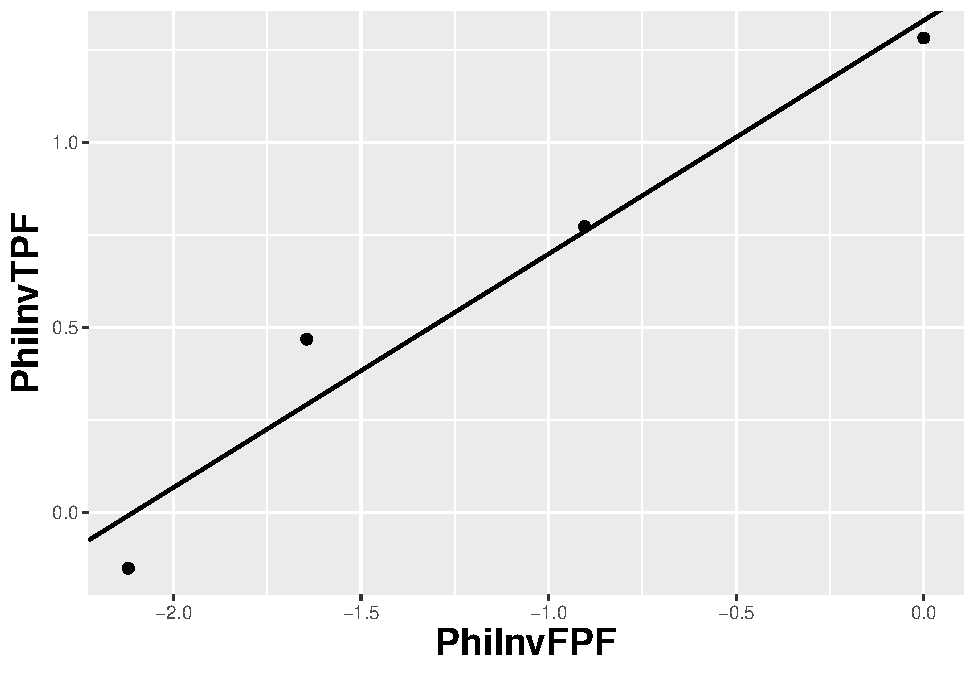
\includegraphics{08-Hypothesis-Testing_files/figure-latex/unnamed-chunk-6-1.pdf}

Line 6 creates two variables, \texttt{muNH} = 1.5 (the binormal model separation parameter under the NH) and \texttt{muAH} = 2.1 (the separation parameter under the AH). Under either hypotheses, the same diseased case standard deviation \texttt{sigma} = 1.3 and 50 non-diseased and 52 diseased cases are assumed. As before, lines 8 -- 14 use the ``brute force'' technique to determine population AUC and standard deviation of AUC under the NH condition. Line 16 defines the number of trials \texttt{T} = 2000. Line 17 creates a vector \texttt{mu} containing the NH and AH values defined at line 6. Line 18 creates \texttt{alphaArr}, a sequence of 10 equally spaced values in the range 0.05 to 0.95, which represent 10 values for \(\alpha\). Line 19 creates two arrays of length 10 each, named \texttt{EmpAlpha} and \texttt{EmpPower}, to hold the values of the observed Type-I error rate, i.e., empirical \(\alpha\), and the empirical power, respectively. The program will run \texttt{T} = 2000 NH and \texttt{T} = 2000 AH trials using as \(\alpha\) each successive value in \texttt{alphaArr} and save the observed Type-I error rates and observed powers to the arrays \texttt{EmpAlpha} and \texttt{EmpPower}, respectively.

The action begins in line 20, which begins a for-loop in \texttt{a}, an index into \texttt{alphaArr.} Line 21 selects the appropriate value for \texttt{alpha} (0.05 on the first pass, 0.15 on the next pass, etc.). Line 22 initializes \texttt{reject{[}2,2000{]}} with zeroes, to hold the result of each trial; the first index corresponds to hypothesis \texttt{h} and the second to trial \texttt{t}. Line 23 begins a for-loop in \texttt{h}, with \texttt{h} = 1 corresponding to the NH and \texttt{h} = 2 to the AH. Line 24 begins a for-loop in \texttt{t}, the trial index. The code within this block is similar to previous examples. It simulates ratings, computes AUC, calculates the p-value, and saves a rejection of the NH as a one at the appropriate array location \texttt{reject{[}h,t{]}}. Lines 32 -- 33 calculate the empirical \(\alpha\) and empirical power for each value of \(\alpha\) in \texttt{alphaArr}. After padding the ends with zero and ones (the trivial points), the remaining lines plot the ``ROC within an ROC''.

Each of the circles in the figure corresponds to a specific value of \(\alpha\). For example the lowest non-trivial corresponds to \(\alpha\) = 0.05, for which the empirical \(\alpha\) is 0.049 and the corresponding empirical Power is 0.4955. True \(\alpha\) increases as the operating point moves up the plot, with empirical \(\alpha\) and empirical power increasing correspondingly. The \(AUC\) under this curve is determined by the effect size, defined as the difference between the AH and NH values of the separation parameter. If the effect size is zero, then the circles will scatter around the chance diagonal; the scatter will be consistent with the 2000 trials used to generate each coordinate of a point. As the effect size increases, the plot approaches the perfect ``ROC'', i.e., approaching the top-left corner. One could use AUC under this ``ROC'' as a measure of the incremental performance, the advantage being that it would be totally independent of \(\alpha\), but this would not be practical as it requires replication of the study under NH and AH conditions about 2000 times each and the entire process has to be repeated for several values of \(\alpha\). The purpose of this demonstration was to illustrate the concept behind Metz's profound remark.

It is time to move on to factors affecting statistical power in a single study.

\hypertarget{factors-affecting-statistical-power}{%
\subsection{Factors affecting statistical power}\label{factors-affecting-statistical-power}}

\begin{itemize}
\tightlist
\item
  Effect size: effect size is defined as the difference in \(AUC_{pop}\) values between the alternative hypothesis condition and the null hypothesis condition. Recall that \(AUC_{pop}\) is defined as the true or population value of the empirical ROC-AUC for the relevant hypothesis. One can use the ``cheat method'' to estimate it under the alternative hypothesis. The formalism is easier if one assumes it is equal to the asymptotic binormal model predicted value. The binormal model yields an estimate of the parameters, which only approach the population values in the asymptotic limit of a large number of cases. In the following, it is assumed that the parameters on the right hand side are the population values)
  It follows that effect size (ES) is given by (all quantities on the right hand side of Eqn. (8.13) are population values):
\end{itemize}

\begin{equation*} 
AUC = \Phi\left ( \frac{ \mu }{\sqrt{ 1 + \sigma^2}} \right )
\end{equation*}

It follows that effect size (ES) is given by (all quantities on the right hand side of above equation are population values):

\begin{equation*} 
ES = \Phi\left ( \frac{\mu_{AH}}{\sqrt{1+\sigma^2}} \right ) - \Phi\left ( \frac{\mu_{NH}}{\sqrt{1+\sigma^2}} \right )
\end{equation*}

\begin{Shaded}
\begin{Highlighting}[]
\NormalTok{EffectSize \textless{}{-}}\StringTok{ }\ControlFlowTok{function}\NormalTok{ (muNH, sigmaNH, muAH, sigmaAH)}
\NormalTok{\{}
\NormalTok{  ES \textless{}{-}}\StringTok{ }\KeywordTok{pnorm}\NormalTok{(muAH}\OperatorTok{/}\KeywordTok{sqrt}\NormalTok{(}\DecValTok{1}\OperatorTok{+}\NormalTok{sigmaAH}\OperatorTok{\^{}}\DecValTok{2}\NormalTok{)) }\OperatorTok{{-}}\StringTok{ }\KeywordTok{pnorm}\NormalTok{(muNH}\OperatorTok{/}\KeywordTok{sqrt}\NormalTok{(}\DecValTok{1}\OperatorTok{+}\NormalTok{sigmaNH}\OperatorTok{\^{}}\DecValTok{2}\NormalTok{))}
  \KeywordTok{return}\NormalTok{ (ES)}
\NormalTok{\}}

\NormalTok{seed \textless{}{-}}\StringTok{ }\DecValTok{1}\NormalTok{;}\KeywordTok{set.seed}\NormalTok{(seed)}
\NormalTok{muAH \textless{}{-}}\StringTok{ }\FloatTok{2.1} \CommentTok{\# NH value, defined previously, was mu = 1.5}

\NormalTok{T \textless{}{-}}\StringTok{ }\DecValTok{2000}
\NormalTok{alpha \textless{}{-}}\StringTok{ }\FloatTok{0.05} \CommentTok{\# size of test}
\NormalTok{reject =}\StringTok{ }\KeywordTok{array}\NormalTok{(}\DecValTok{0}\NormalTok{, }\DataTypeTok{dim =}\NormalTok{ T)}
\ControlFlowTok{for}\NormalTok{ (t }\ControlFlowTok{in} \DecValTok{1}\OperatorTok{:}\KeywordTok{length}\NormalTok{(reject)) \{  }
\NormalTok{  zk1 \textless{}{-}}\StringTok{ }\KeywordTok{rnorm}\NormalTok{(K1);zk2 \textless{}{-}}\StringTok{ }\KeywordTok{rnorm}\NormalTok{(K2, }\DataTypeTok{mean =}\NormalTok{ muAH, }\DataTypeTok{sd =}\NormalTok{ sigma)  }
\NormalTok{  AUC \textless{}{-}}\StringTok{ }\KeywordTok{Wilcoxon}\NormalTok{(zk1, zk2)  }
\NormalTok{  obsvdZ \textless{}{-}}\StringTok{ }\NormalTok{(AUC }\OperatorTok{{-}}\StringTok{ }\NormalTok{meanAUC)}\OperatorTok{/}\NormalTok{sigmaAUC}
\NormalTok{  p \textless{}{-}}\StringTok{ }\DecValTok{2}\OperatorTok{*}\KeywordTok{pnorm}\NormalTok{(}\OperatorTok{{-}}\KeywordTok{abs}\NormalTok{(obsvdZ)) }\CommentTok{\# p value for individual t}
  \ControlFlowTok{if}\NormalTok{ (p }\OperatorTok{\textless{}}\StringTok{ }\NormalTok{alpha) reject[t] =}\StringTok{ }\DecValTok{1} 
\NormalTok{\}}

\NormalTok{ObsvdTypeIErrRate \textless{}{-}}\StringTok{ }\KeywordTok{sum}\NormalTok{(reject)}\OperatorTok{/}\KeywordTok{length}\NormalTok{(reject)}
\NormalTok{CI \textless{}{-}}\StringTok{ }\KeywordTok{c}\NormalTok{(}\DecValTok{0}\NormalTok{,}\DecValTok{0}\NormalTok{);width \textless{}{-}}\StringTok{ }\OperatorTok{{-}}\KeywordTok{qnorm}\NormalTok{(alpha}\OperatorTok{/}\DecValTok{2}\NormalTok{)}
\NormalTok{CI[}\DecValTok{1}\NormalTok{] \textless{}{-}}\StringTok{ }\NormalTok{ObsvdTypeIErrRate }\OperatorTok{{-}}\StringTok{ }
\StringTok{  }\NormalTok{width}\OperatorTok{*}\KeywordTok{sqrt}\NormalTok{(ObsvdTypeIErrRate}\OperatorTok{*}\NormalTok{(}\DecValTok{1}\OperatorTok{{-}}\NormalTok{ObsvdTypeIErrRate)}\OperatorTok{/}\NormalTok{T)}
\NormalTok{CI[}\DecValTok{2}\NormalTok{] \textless{}{-}}\StringTok{ }\NormalTok{ObsvdTypeIErrRate }\OperatorTok{+}\StringTok{ }
\StringTok{  }\NormalTok{width}\OperatorTok{*}\KeywordTok{sqrt}\NormalTok{(ObsvdTypeIErrRate}\OperatorTok{*}\NormalTok{(}\DecValTok{1}\OperatorTok{{-}}\NormalTok{ObsvdTypeIErrRate)}\OperatorTok{/}\NormalTok{T)}
\KeywordTok{cat}\NormalTok{(}\StringTok{"obsvdPower = "}\NormalTok{, ObsvdTypeIErrRate, }\StringTok{"}\CharTok{\textbackslash{}n}\StringTok{"}\NormalTok{)}
\CommentTok{\#\textgreater{} obsvdPower =  0.489}
\KeywordTok{cat}\NormalTok{(}\StringTok{"95\% confidence interval = "}\NormalTok{, CI, }\StringTok{"}\CharTok{\textbackslash{}n}\StringTok{"}\NormalTok{)}
\CommentTok{\#\textgreater{} 95\% confidence interval =  0.4670922 0.5109078}
\KeywordTok{cat}\NormalTok{(}\StringTok{"Effect Size = "}\NormalTok{, }\KeywordTok{EffectSize}\NormalTok{(mu, sigma, muAH, sigma), }\StringTok{"}\CharTok{\textbackslash{}n}\StringTok{"}\NormalTok{)}
\CommentTok{\#\textgreater{} Effect Size =  0.08000617 0}
\end{Highlighting}
\end{Shaded}

The ES for the code above is 0.08 (in AUC units). It should be obvious that if effect size is zero, then power equals \(\alpha\). This is because then there is no distinction between the null and alternative hypotheses conditions. Conversely, as effect size increases, statistical power increases, the limiting value being unity, when every trial results in rejection of the null hypothesis. The reader should experiment with different values of \texttt{muAH} to be convinced of the truth of these statements.

\begin{itemize}
\tightlist
\item
  Sample size: increase the number of cases by a factor of two, and run the above code chunk.
\end{itemize}

\begin{verbatim}
#> pop NH mean AUC =  0.8594882 , pop NH sigma AUC =  0.02568252
#> num. non-diseased images =  100 num. diseased images =  104
#> obsvdPower =  0.313
#> 95% confidence interval =  0.2926772 0.3333228
#> Effect Size =  0.08000617 0
\end{verbatim}

So doubling the numbers of cases (both non-diseased and diseased) results in statistical power increasing from 0.509 to 0.844. Increasing the numbers of cases decreases \(\sigma_{AUC}\), the standard deviation of the empirical AUC. The new value of \(\sigma_{AUC}\) is 0.02947, which should be compared to the value 0.04177 for K1 = 50, K2 = 52. Recall that \(\sigma_{AUC}\) enters the denominator of the Z-statistic, so decreasing it will increase the probability of rejecting the null hypothesis.

\begin{itemize}
\tightlist
\item
  Alpha: Statistical power depends on \(alpha\). return the sample size to the original values . The results below are for two runs of the code, the first with the original value , set at line 16, the second with :
\end{itemize}

\begin{verbatim}
#> alpha =  0.05 obsvdPower =  0.1545 
#> alpha =  0.01 obsvdPower =  0.0265
\end{verbatim}

Decreasing \(\alpha\) results in decreased statistical power.

\hypertarget{comments}{%
\section{Comments}\label{comments}}

The Wilcoxon statistic was used to estimate the area under the ROC curve. One could have used the binormal model, introduced in Chapter 06, to obtain maximum likelihood estimates of the area under the binormal model fitted ROC curve. The reasons for choosing the simpler empirical area are as follows. (1) With continuous ratings and 102 operating points, the area under the empirical ROC curve is expected to be a close approximation to the fitted area. (2) With maximum likelihood estimation, the code would be more complex -- in addition to the fitting routine one would require a binning routine and that would introduce yet another variable in the analysis, namely the number of bins and how the bin boundaries were chosen. (3) The maximum likelihood fitting code can sometimes fail to converge, while the Wilcoxon method is always guaranteed to yield a result. The non-convergence issue is overcome by modern methods of curve fitting described in later chapters. (4) The aim was to provide an understanding of null hypothesis testing and statistical power without being bogged down in the details of curve fitting.

\hypertarget{why-alpha-is-chosen-to-be-5}\label{why-alpha-is-chosen-to-be-5}}

One might ask why \(\alpha\) is traditionally chosen to be 5\%. It is not a magical number, rather a cost benefit tradeoff. Choosing too small a value of \(\alpha\) would result in greater probability \((1-\alpha)\) of the NH not being rejected, even when it is false, i.e., decreased power. Sometimes it is important to detect a true difference between the measured AUC and the postulated value. For example, a new eye-laser surgery procedure is invented and the number of patients is necessarily small as one does not wish to subject a large number of patients to an untried procedure. One seeks some leeway on the Type-I error probability, possibly increasing it to \(\alpha\) = 0.1, in order to have a reasonable chance of success in detecting an improvement in performance due to better eyesight after the surgery. If the NH is rejected and the change is in the right direction, then that is good news for the researcher. One might then consider a larger clinical trial and set \(\alpha\) at the traditional 0.05, making up the lost statistical power by increasing the number of patients on which the surgery is tried.

If a whole branch of science hinges on the results of a study, such as discovering the Higg's Boson in particle physics, statistical significance is often expressed in multiples of the standard deviation (\(\sigma\)) of the normal distribution, with the significance threshold set at a much stricter level (e.g.~\(5\sigma\)). This corresponds to \(\alpha\) \textasciitilde{} 1 in 3.5 million (\texttt{1/pnorm(-5)} = 3.5 x 10\^{}6, a one-sided test of significance). There is an article in Scientific American (\url{https://blogs.scientificamerican.com/observations/five-sigmawhats-that/}) on the use of \(n\sigma\), where \texttt{n} is an integer, e.g.~5, to denote the significance level of a study, and some interesting anecdotes on why such high significance levels (low alpha) are used in some fields of research.

Similar concerns apply to manufacturing where the cost of a mistake could be the very expensive recall of an entire product line. For background on Six Sigma Performance, see \url{http://www.six-sigma-material.com/Six-Sigma.html}. An article downloaded 3/30/17 from \url{https://en.wikipedia.org/wiki/Six_Sigma} is included as supplemental material to this chapter (Six Sigma.pdf). It has an explanation of why \(6\sigma\) translates to one defect per 3.4 million opportunities (it has to do with short-term and long-term drifts in a process). In the author's opinion, looking at other fields offers a deeper understanding of this material than simply stating that by tradition one adopts alpha = 5\%.

Most observer performance studies, while important in the search for better imaging methods, are not of such ``earth-shattering'' importance, and it is somewhat important to detect true differences (AH is true) at a reasonable alpha, so alpha = 5\% and beta = 20\% represent a good compromise. If one adopted a \(5\sigma\) criterion, the NH would never be rejected, and progress in image quality optimization would come to a grinding halt. That is not to say that a \(5\sigma\) criterion cannot be used; rather if used, the number of patients needed to detect a reasonable difference (effect size) with 80\% probability would be astronomically large. Truth-proven cases are a precious commodity in observer performance studies. Particle physicists working on discovering the Higg's Boson can get away with \(5\sigma\) criterion because the number of independent observations and/or effect size is much larger than corresponding numbers in observer performance research.

\hypertarget{discussion}{%
\section{Discussion}\label{discussion}}

In most statistics books, the subject of hypothesis testing is demonstrated in different (i.e., non-ROC) contexts. That is to be expected since the ROC-analysis field is a very small subspecialty of statistics (Prof.~Howard E. Rockette, private communication, ca. 2002). Since this book is about ROC analysis, the author decided to use a demonstration using ROC analysis. Using a data simulator, one is allowed to ``cheat'' by conducting a very large number of simulations to estimate the population \(AUC\) under the null hypothesis. This permitted us to explore the related concepts of Type-I and Type-II errors within the context of ROC analysis. Ideally, both errors should be zero, but the nature of statistics leads one to two compromises. Usually one accepts a Type-I error capped at 5\% and a Type-II error capped at 20\%. These translate to \(\alpha\) = 0.05 and desired statistical power = 80\%. The dependence of statistical power on \(\alpha\), the numbers of cases and the effect size was explored. Statistical power increases with the effect size, it increases with \(\alpha\) and it increases with the sample size (numbers of cases).

In Chapter 11 sample-size calculations are described that allow one to estimate the numbers of readers and cases needed to detect a specified difference in inter-modality AUCs with an expected statistical power \(1-\beta\) . The word ``detect'' in the preceding sentence is shorthand for ``reject the NH with probability capped at \(\alpha\) while also rejecting the alternative hypothesis with probability capped at \(\beta\)''.

This chapter also gives the first example of validation of a hypothesis testing method. Statisticians sometimes refer to this as showing a proposed test is a ``5\% test''. What is meant is that one needs to be assured that when the NH is true the probability of NH rejection equals the expected value, namely \(\alpha\), typically chosen to be 5\%. Since the observed NH rejection rate over 2000 simulations is a random variable, one does not expect the NH rejection rate to exactly equal 5\%, rather the constructed 95\% confidence interval (also a random interval variable) should include the NH value with probability \(\alpha\).

As noted in the introduction, comparing a single reader's performance to a specified value is not a clinically interesting problem. The next two chapters describe methods for significance testing of multiple-reader multiple-case (MRMC) ROC datasets, consisting of interpretations by a group of readers of a common set of cases in typically two modalities. It turns out that the analyses yield variability estimates that permit sample size calculation. After all, sample size calculation is all about estimation of variability, the denominator of the z-statistic, i.e., Eqn. (8.3), in the context of this chapter. The formulae will look more complex, as interest is not in determining the standard deviation of AUC, but in the standard deviation of the inter-modality reader-averaged AUC difference. However, the basic concepts remain the same.

\hypertarget{references}{%
\section{References}\label{references}}

\hypertarget{DBMAnalysisBkgrnd}{%
\chapter{Background on Dorfman Berbaum Metz (DBM) Analysis}\label{DBMAnalysisBkgrnd}}

\hypertarget{introduction}{%
\section{Introduction}\label{introduction}}

In this chapter the term ``treatment'' is used as a generic for ``imaging system'', ``modality'' or ``image processing'' and ``reader'' is used as a generic for ``radiologist'' or algorithmic observer, e.g., a computer aided detection (CAD) algorithm. In the context of illustrating hypothesis-testing methods the previous chapter described analysis of a single ROC dataset and comparing the observed area \(AUC\) under the ROC plot to a specified value. Clinically this is not the most interesting problem; rather, interest is usually in comparing performance of a group of readers interpreting a common set of cases in two or more treatments. Such data is termed multiple reader multiple case (MRMC). {[}An argument could be made in favor of the term ``multiple-treatment multiple-reader'', since ``multiple-case'' is implicit in any ROC analysis that takes into account correct and incorrect decisions on cases. However, the author will stick with existing terminology.{]} The basic idea is that by sampling a sufficiently large number of readers and a sufficiently large number of cases one might be able to draw conclusions that apply broadly to other readers of similar skill levels interpreting other similar case sets in the selected treatments. How one accomplishes this, termed MRMC analysis, is the subject of this chapter.

This chapter describes the first truly successful method of analyzing MRMC ROC data, namely the Dorfman-Berbaum-Metz (DBM) method \citep{RN204}. The other method, due to Obuchowski and Rockette \citep{RN1450}, is the subject of Chapter 10. Both methods have been substantially improved by Hillis \citep{RN1866, RN1865, RN2508}. Hence the title of this chapter: ``Dorfman Berbaum Metz Hillis (DBM) Analysis''. It is not an overstatement that ROC analysis came of age with the methods described in this chapter. Prior to the techniques described here, one knew of the existence of sources of variability affecting a measured \(AUC\) value, as discussed in (book) Chapter 07, but then-known techniques \citep{RN412} for estimating the corresponding variances and correlations were impractical.

\hypertarget{historical-background}{%
\subsection{Historical background}\label{historical-background}}

The author was thrown (unprepared) into the methodology field ca. 1985 when, as a junior faculty member, he undertook comparing a prototype digital chest-imaging device (Picker International, ca. 1983) vs.~an optimized analog chest-imaging device at the University of Alabama at Birmingham. At the outset a decision was made to use free-response ROC methodology instead of ROC, as the former accounted for lesion localization, and the author and his mentor, Prof.~Gary T. Barnes, were influenced in that decision by a publication \citep{RN2453} to be described in (book) Chapter 12. Therefore, instead of ROC-AUC one had lesion-level sensitivity at a fixed number of location level false positives per case as the figure-of-merit (FOM). Details of the FOM are not relevant at this time. Suffice to state that methods described in this chapter, which had not been developed in 1983, while developed for analyzing reader-averaged inter-treatment ROC-AUC differences, \emph{apply to any scalar FOM}. While the author was successful at calculating confidence intervals (this is the heart of what is loosely termed ``statistical analysis'') and publishing the work \citep{RN621} using techniques described in a book \citep{RN412} titled ``Evaluation of Diagnostic Systems: Methods from Signal Detection Theory'', subsequent attempts at applying these methods in a follow-up paper \citep{RN620} led to negative variance estimates (private communication, Dr.~Loren Niklason, ca. 1985). With the benefit of hindsight, negative variance estimates are not that uncommon and the method to be described in this chapter has to deal with that possibility.

The methods \citep{RN412} described in the cited book involved estimating the different variability components -- case sampling, between-reader and within-reader variability. Between-reader and within-reader variability (the two cannot be separated as discussed in (book) Chapter 07) could be estimated from the variance of the \(AUC\) values corresponding to the readers interpreting the cases within a treatment and then averaging the variances over all treatments. Estimating case-sampling and within-reader variability required splitting the dataset into a few smaller subsets (e.g., a case set with 60 cases might be split into 3 sub-sets of 20 cases each), analyzing each subset to get an \(AUC\) estimate and calculating the variance of the resulting \(AUC\) values \citep{RN412} and scaling the result to the original case size. Because it was based on few values, the estimate was inaccurate, and the already case-starved original dataset made it difficult to estimate AUCs for the subsets; moreover, the division into subsets was at the discretion of the researcher, and therefore unlikely to be reproduced by others. Estimating within-reader variability required re-reading the entire case set, or at least a part of it. ROC studies have earned a deserved reputation for taking much time to complete, and having to re-read a case set was not a viable option. {[}Historical note: the author recalls a barroom conversation with Dr.~Thomas Mertelmeir after the conclusion of an SPIE meeting ca. 2004, where Dr.~Mertelmeir commiserated mightily, over several beers, about the impracticality of some of the ROC studies required of imaging device manufacturers by the FDA.{]}

\hypertarget{the-wagner-analogy}{%
\subsection{The Wagner analogy}\label{the-wagner-analogy}}

An important objective of modality comparison studies is to estimate the variance of the difference in reader-averaged AUCs between the treatments. For two treatments one sums the reader-averaged variance in each treatment and subtracts twice the covariance (a scaled version of the correlation). Therefore, in addition to estimating variances, one needs to estimate correlations. Correlations are present due to the common case set interpreted by the readers in the different treatments. If the correlation is large, i.e., close to unity, then the individual treatment variances tend to cancel, making the constant treatment-induced difference easier to detect. The author recalls a vivid analogy used by the late Dr.~Robert F. Wagner to illustrate this point at an SPIE meeting ca. 2008. To paraphrase him, \emph{consider measuring from shore the heights of the masts on two adjacent boats in a turbulent ocean. Because of the waves, the heights, as measured from shore, are fluctuating wildly, so the variance of the individual height measurements is large. However, the difference between the two heights is likely to be relatively constant, i.e., have small variance. This is because the wave that causes one mast's height to increase also increases the height of the other mast.}

\hypertarget{the-shortage-of-numbers-to-analyze-and-a-pivotal-breakthrough}{%
\subsection{The shortage of numbers to analyze and a pivotal breakthrough}\label{the-shortage-of-numbers-to-analyze-and-a-pivotal-breakthrough}}

\emph{The basic issue was that the calculation of \(AUC\) reduces the relatively large number of ratings of a set of non-diseased and diseased cases to a single number.} For example, after completion of an ROC study with 5 readers and 100 non-diseased and 100 diseased cases interpreted in two treatments, the data is reduced to just 10 numbers, i.e., five readers times two treatments. It is difficult to perform statistics with so few numbers. The author recalls a conversation with Prof.~Kevin Berbaum at a Medical Image Perception Society meeting in Tucson, Arizona, ca. 1997, in which he described the basic idea that forms the subject of this chapter. Namely, using the jackknife pseudovalues (to be defined below) as individual case-level figures of merit. This, of course, greatly increases the amount of data that one can work with; instead of just 10 numbers one now has 2,000 pseudovalues (2 x 5 x 200). If one assumes the pseudovalues behave essentially as case-level data, then by assumption they are independent and identically distributed, and therefore they satisfy the conditions for application of standard analysis of variance (ANOVA) techniques. {[}This assumption has been much criticized and is the basis for some preferring alternate approaches - but, as Hillis has stated, and I paraphrase, the pseudovalue based method ``works'', but lacks sufficient rigor.{]} The relevant paper had already been published in 1992 but other distractions and lack of formal statistical training kept the author from fully appreciating this work until later.

Although methods are available for more complex study designs including partially paired data \citep{RN2128, RN1880}, I will restrict to fully paired data (i.e., each case is interpreted by all readers in all treatments). There is a long history of how this field has evolved and the author cannot do justice to all methods that are currently available. Some of the methods \citep{RN1441, RN2013, RN1451} have the advantage that they can handle explanatory variables (termed covariates) that could influence performance, e.g., years of experience, types of cases, etc. Other methods are restricted to specific choices of FOM. Specifically, the probabilistic approach \citep{RN2253, RN2254, RN2351, RN2080} is restricted to the empirical \(AUC\) under the ROC curve, and therefore are not applicable to other FOMs, e.g., parametrically fitted ROC AUCs or, more importantly, to location specific paradigm FOMs. Instead, the author will focus on methods for which software is readily available (i.e., freely on websites), which have been widely used (the method that the author is about to describe has been used in several hundred publications) and validated via simulations, and which apply to any scalar figure of merit, and therefore widely applicable, even to location specific paradigms.

\hypertarget{organization-of-the-chapter}{%
\subsection{Organization of the chapter}\label{organization-of-the-chapter}}

The organization of the chapter is as follows. The concepts of reader and case populations, introduced in (book) Chapter 07, are recapitulated. A distinction is made between \emph{fixed} and \emph{random} factors -- statistical terms with which one must become familiar. Described next are three types of analysis that are possible with MRMC data, depending on which factors are regarded as random and which as fixed. The general approach to the analysis is described. Two methods of analysis are possible: the jackknife pseudovalue-based approach detailed in this chapter and an alternative approach is detailed in Chapter 10. The Dorfman-Berbaum-Metz (DBM) model for the jackknife pseudovalues is described that incorporates different sources of variability and correlations possible with MRMC data. Calculation of ANOVA-related quantities, termed mean squares, from the pseudovalues, are described followed by the significance testing procedure for testing the null hypothesis of no treatment effect. A relevant distribution used in the analysis, namely the F-distribution, is illustrated with R examples. The decision rule, i.e., whether to reject the NH, calculation of the ubiquitous p-value, confidence intervals and how to handle multiple treatments is illustrated with two datasets, one an older ROC dataset that has been widely used to demonstrate advances in ROC analysis, and the other a recent dataset involving evaluation of digital chest tomosynthesis vs.~conventional chest imaging. The approach to validation of DBM analysis is illustrated with an R example. The chapter concludes with a section on the meaning of the pseudovalues. The intent is to explain, at an intuitive level, why the DBM method ``works'', even though use of pseudovalues has been questioned3 at the conceptual level. For organizational reasons and space limitations, details of the software are relegated to Online Appendices, but they are essential reading, preferably in front of a computer running the online software that is part of this book. The author has included material here that may be obvious to statisticians, e.g., an explanation of the Satterthwaite approximation, but are expected to be helpful to others from non-statistical backgrounds.

\hypertarget{random-and-fixed-factors}{%
\section{Random and fixed factors}\label{random-and-fixed-factors}}

\emph{This paragraph introduces some analysis of variance (ANOVA) terminology. Treatment, reader and case are factors with different numbers of levels corresponding to each factor. For an ROC study with two treatments, five readers and 200 cases, there are two levels of the treatment factor, five levels of the reader factor and 200 levels of the case factor. If a factor is regarded as fixed, then the conclusions of the analysis apply only to the specific levels of the factor used in the study. If a factor is regarded as random, the levels of the factor are regarded as random samples from a parent population of the corresponding factor and conclusions regarding specific levels are not allowed; rather, conclusions apply to the distribution from which the levels are, by assumption, sampled.}

ROC MRMC studies require a sample of cases and interpretations by one or more readers in one or more treatments (in this book the term ``multiple'' includes as a special case ``one''). A study is never conducted on a sample of treatments. It would be nonsensical to image patients using a ``sample'' of all possible treatments known to exist. Every variation of an imaging technique (e.g., different kilovoltage or kVp) or display method (e.g., window-level setting) or image processing techniques qualifies as a distinct treatment. The number of possible treatments is very large, and, from a practical point of view, most of them are uninteresting. Rather, interest is in comparing two or more (a few at most) treatments that, based on preliminary studies, are clinically interesting. One treatment may be computed tomography, the other magnetic resonance imaging, or one may be interested in comparing a standard image processing method to a newly proposed one, or one may be interested in comparing CAD to a group of readers.

This brings out an essential difference between how cases, readers and treatments have to be regarded in the variability estimation procedure. Cases and readers are usually regarded as random factors (there has to be at least one random factor -- if not, there are no sources of variability and nothing to apply statistics to!), while treatments are regarded as fixed factors. The random factors contribute stochastic (i.e., random) variability, but the fixed factors do not, rather they contribute constant shifts in performance. The terms fixed and random factors are used in this specific sense, and are derived, in turn, from ANOVA methods in statistics10,25. With two or more treatments, there are shifts in performance of treatments relative to each other, that one seeks to assess the significance of against a background of noise contributed by the random factors. If the shifts are sufficiently large compared to the noise, then one can state, with some certainty, that they are real. Quantifying the last statement uses the methods of hypothesis testing introduced in Chapter \ref{HypothesisTesting} or Chapter {[}Hypothesis Testing{]}.

\hypertarget{reader-and-case-populations-and-data-correlations}{%
\section{Reader and case populations and data correlations}\label{reader-and-case-populations-and-data-correlations}}

As discussed in (book) §7.2, conceptually there is a reader-population, generally modeled as a normal distribution \(\theta_j \sim N\left ( \theta_{\bullet\{1\}}, \sigma_{br+wr}^{2} \right )\), describing the variation of skill-level of readers. The notation closely follows that in the cited section, the only change being that the binormal model estimate \(A_z\) has been replaced by a generic FOM, denoted \(\theta\). Each reader \(j\) is characterized by a different value of \(\theta_j\), \(j=1,2,...J\) and one can conceptually think of a bell-shaped curve with variance \(\sigma_{br+wr}^{2}\) describing between-reader variability of the readers. A large variance implies large spread in reader skill levels.

Likewise, there is a case-population, also modeled as a normal distribution, describing the variations in difficulty levels of the patients. One actually has two unit-variance distributions, one per diseased state, characterized by a separation parameter and conceptually an easy case set has a larger than usual separation parameter while a difficult case set has a smaller than usual separation parameter. The distribution of the separation parameter can be modeled as a bell-shaped curve \(\theta_{\{c\}} \sim N\left ( \theta_{\{\bullet\}}, \sigma_{cs+wr}^{2} \right )\) with variance \(\sigma_{cs+wr}^{2}\) describing the variations in difficulty levels of different case samples. Note the need for the case-set index, introduced in Chapter 07, to specify the separation parameter for a specific case-set (in principle a \(j\)-index is also needed as one cannot have an interpretation without a reader; for now it is suppressed; one can think of the stated equation as applying to the average reader). A small variance \(\sigma_{cs}^{2}\) implies the different case sets have similar difficulty levels while a larger variance would imply a larger spread in difficulty levels.

\emph{Anytime one has a common random component to two measurements, the measurements are correlated.} In the Wagner analogy, the common component is the random height, as a function of time, of a wave, which contributes the same amount to both height measurements (since the boats are adjacent). Since the readers interpret a common case set in all treatments one needs to account for various types of correlations that are potentially present. These occur due to the various types of pairings that can occur with MRMC data, where each pairing implies the presence of a common component to the measurements: (a) the same reader interpreting the same cases in different treatments, (b) different readers interpreting the same cases in the same treatment and (c) different readers interpreting the same cases in different treatments. These pairings are more clearly elucidated in (book) Chapter 10. The current chapter uses jackknife pseudovalue based analysis to model the variances and the correlations. Hillis has shown that the two approaches are essentially equivalent \citep{RN1866}.

\hypertarget{three-types-of-analyses}{%
\section{Three types of analyses}\label{three-types-of-analyses}}

\emph{MRMC analysis attempts to draw conclusions regarding the significances of inter-treatment shifts in performance. Ideally a conclusion (i.e., a difference is significant: yes/no; the ``yes'' applies if the p-value is less than alpha) should generalize to the respective populations from which the random samples were obtained. In other words, the idea is to generalize from the observed samples to the underlying populations. Three types of analyses are possible depending on which factor(s) one regards as random and which as fixed: random-reader random-case (RRRC), fixed-reader random-case (FRRC) and random-reader fixed-case (RRFC). If a factor is regarded as random, then the conclusion of the study applies to the population from which the levels of the factor were sampled. If a factor is regarded as fixed, then the conclusion applies only to the specific levels of the sampled factor. For example, if reader is regarded as a random factor, the conclusion generalizes to the reader population from which the readers used in the study were obtained. If reader is regarded as a fixed factor, then the conclusion applies to the specific readers that participated in the study. Regarding a factor as fixed effectively ``freezes out'' the sampling variability of the population and interest then centers only on the specific levels of the factor used in the study. For fixed reader analysis, conclusions about the significances of differences between pairs of readers are allowed; these are not allowed if reader is treated as a random factor. Likewise, treating case as a fixed factor means the conclusion of the study is specific to the case-set used in the study.}

\hypertarget{general-approach}{%
\section{General approach}\label{general-approach}}

This section provides an overview of the steps involved in analysis of MRMC data. Two approaches are described in parallel: a figure of merit (FOM) derived jackknife pseudovalue based approach, detailed in this chapter and an FOM based approach, detailed in the next chapter. The analysis proceeds as follows:

\begin{enumerate}
\def\labelenumi{\arabic{enumi}.}
\tightlist
\item
  A FOM is selected: \emph{the selection of FOM is the single-most critical aspect of analyzing an observer performance study}. The selected FOM is denoted \(\theta\). To keep the notation reasonably compact the usual circumflex ``hat'' symbol used previously to denote an estimate is suppressed. The FOM has to be an objective scalar measure of performance with larger values characterizing better performance. {[}The qualifier ``larger'' is trivially satisfied; if the figure of merit has the opposite characteristic, a sign change is all that is needed to bring it back to compliance with this requirement.{]} Examples are empirical \(AUC\), the binormal model-based estimate \(A_z\) , other advance method based estimates of \(AUC\), sensitivity at a predefined value of specificity, etc. An example of a FOM requiring a sign-change is \(FPF\) at a specified \(TPF\), where smaller values signify better performance.
\item
  For each treatment \(i\) and reader \(j\) the figure of merit \(\theta_{ij}\) is estimated from the ratings data. Repeating this over all treatments and readers yields a matrix of observed values \(\theta_{ij}\). This is averaged over all readers in each treatment yielding \(\theta_{i\bullet}\). The observed effect-size \(ES_{obs}\) is defined as the difference between the reader-averaged FOMs in the two treatments, i.e., \(ES_{obs}\) = \(\theta_{2\bullet}\) - \(\theta_{1\bullet}\). While extensible to more than two treatments, the explanation is more transparent by restricting to two modalities.
\item
  If the magnitude of \(ES_{obs}\) is ``large'' one has reason to suspect that there might indeed be a significant difference in AUCs between the two treatments, where significant is used in the sense of (book) Chapter 08. Quantification of this statement, specifically how large is ``large'', requires the conceptually more complex steps described next.
\end{enumerate}

\begin{itemize}
\tightlist
\item
  In the DBM approach, the subject of this chapter, jackknife pseudovalues are calculated as described in Chapter 08. A standard ANOVA model with uncorrelated errors is used to model the pseudovalues.
\item
  In the OR approach, the subject of the next chapter, the FOM is modeled directly using a custom ANOVA model with correlated errors.
\end{itemize}

\begin{enumerate}
\def\labelenumi{\arabic{enumi}.}
\tightlist
\item
  Depending on the selected method of modeling the data (pseudovalue vs.~FOM) a statistical model is used which includes parameters modeling the true values in each treatment, and expected variations due to different variability components in the model, e.g., between-reader variability, case-sampling variability, interactions (e.g., modeling the possibility that the random effect of a given reader could be treatment dependent) and the presence of correlations (between pseudovalues or FOMs) because of the pairings inherent in the interpretations.
\item
  In RRRC analysis one accounts for randomness in readers and cases. In FRRC analysis one regards reader as a fixed factor. In RRFC analysis one regards case as a fixed factor. The statistical model depends on the type of analysis.
\item
  The parameters of the statistical model are estimated from the observed data.
\item
  The estimates are used to infer the statistical distribution of the observed effect size, \(ES_{obs}\), regarded as a realization of a random variable, under the null hypothesis (NH) that the true effect size is zero.
\item
  Based on this statistical distribution, and assuming a two-sided test, the probability (this is the oft-quoted p-value) of obtaining an effect size at least as extreme as that actually observed, is calculated, as in Chapter 08.
\item
  If the p-value is smaller than a preselected value, denoted \(\alpha\), one declares the treatments different at the \(\alpha\) - significance level. The quantity \(\alpha\) is the control (or cap) on the probability of making a Type I error, defined as rejecting the NH when it is true. It is common to set \(\alpha\) = 0.05 but depending on the severity of the consequences of a Type I error, as discussed in (book) Chapter 08, one might consider choosing a different value. Notice that \(\alpha\) is a pre-selected number while the p-value is a realization of a random variable.
\item
  For a valid statistical analysis, the empirical probability \(\alpha_{emp}\) over many (typically 2000) independent NH datasets, that the p-value is smaller than \(\alpha\), should equal \(\alpha\) to within statistical uncertainty.
\end{enumerate}

\hypertarget{summary-tba}{%
\section{Summary TBA}\label{summary-tba}}

This chapter has detailed analysis of MRMC ROC data using the DBM method. A reason for the level of detail is that almost all of the material carries over to other data collection paradigms, and a thorough understanding of the relatively simple ROC paradigm data is helpful to understanding the more complex ones.

DBM has been used in several hundred ROC studies (Prof.~Kevin Berbaum, private communication ca. 2010). While the method allows generalization of a study finding, e.g., rejection of the NH, to the population of readers and cases, the author believes this is sometimes taken too literally. If a study is done at a single hospital, then the radiologists tend to be more homogenous as compared to sampling radiologists from different hospitals. This is because close interactions between radiologists at a hospital tend to homogenize reading styles and performance. A similar issue applies to patient characteristics, which are also expected to vary more between different geographical locations than within a given location served by the hospital. This means is that single hospital study based p-values may tend to be biased downwards, declaring differences that may not be replicable if a wider sampling ``net'' were used using the same sample size. The price paid for a wider sampling net is that one must use more readers and cases to achieve the same sensitivity to genuine treatment effects, i.e., statistical power (i.e., there is no ``free-lunch'').

A third MRMC ROC method, due to Clarkson, Kupinski and Barrett19,20, implemented in open-source JAVA software by Gallas and colleagues22,44 (\url{http://didsr.github.io/iMRMC/}) is available on the web. Clarkson et al19,20 provide a probabilistic rationale for the DBM model, provided the figure of merit is the empirical \(AUC\). The method is elegant but it is only applicable as long as one is using the empirical AUC as the figure of merit (FOM) for quantifying observer performance. In contrast the DBM approach outlined in this chapter, and the approach outlined in the following chapter, are applicable to any scalar FOM. Broader applicability ensures that significance-testing methods described in this, and the following chapter, apply to other ROC FOMs, such as binormal model or other fitted AUCs, and more importantly, to other observer performance paradigms, such as free-response ROC paradigm. An advantage of the Clarkson et al.~approach is that it predicts truth-state dependence of the variance components. One knows from modeling ROC data that diseased cases tend to have greater variance than non-diseased ones, and there is no reason to suspect that similar differences do not exist between the variance components.

Testing validity of an analysis method via simulation testing is only as good as the simulator used to generate the datasets, and this is where current research is at a bottleneck. The simulator plays a central role in ROC analysis. In the author's opinion this is not widely appreciated. In contrast, simulators are taken very seriously in other disciplines, such as cosmology, high-energy physics and weather forecasting. The simulator used to validate3 DBM is that proposed by Roe and Metz39 in 1997. This simulator has several shortcomings. (a) It assumes that the ratings are distributed like an equal-variance binormal model, which is not true for most clinical datasets (recall that the b-parameter of the binormal model is usually less than one). Work extending this simulator to unequal variance has been published3. (b) It does not take into account that some lesions are not visible, which is the basis of the contaminated binormal model (CBM). A CBM model based simulator would use equal variance distributions with the difference that the distribution for diseased cases would be a mixture distribution with two peaks. The radiological search model (RSM) of free-response data, Chapter 16 \&17 also implies a mixture distribution for diseased cases, and it goes farther, as it predicts some cases yield no z-samples, which means they will always be rated in the lowest bin no matter how low the reporting threshold. Both CBM and RSM account for truth dependence by accounting for the underlying perceptual process. (c) The Roe-Metz simulator is out dated; the parameter values are based on datasets then available (prior to 1997). Medical imaging technology has changed substantially in the intervening decades. (d) Finally, the methodology used to arrive at the proposed parameter values is not clearly described. Needed is a more realistic simulator, incorporating knowledge from alternative ROC models and paradigms that is calibrated, by a clearly defined method, to current datasets.

Since ROC studies in medical imaging have serious health-care related consequences, no method should be used unless it has been thoroughly validated. Much work still remains to be done in proper simulator design, on which validation is dependent.

\hypertarget{references}{%
\section{References}\label{references}}

\hypertarget{DBMAnalysisSigtesting}{%
\chapter{Significance Testing using the DBM Method}\label{DBMAnalysisSigtesting}}

DBM = Dorfman Berbaum Metz

\hypertarget{the-dbm-sampling-model}{%
\section{The DBM sampling model}\label{the-dbm-sampling-model}}

The figure-of-merit has three indices:\\
* A treatment index \(i\), where \(i\) runs from 1 to \(I\), where \(I\) is the total number of treatments.\\
* A reader index \(j\), where \(j\) runs from 1 to \(J\), where \(J\) is the total number of readers.\\
* The case-sample index \(\{c\}\), where \(\{1\}\) i.e., \(c\) = 1, denotes a set of cases, \(K_1\) non-diseased and \(K_2\) diseased, interpreted by all readers in all treatments, and other integer values of \(c\) correspond to other independent sets of cases that, although not in fact interpreted by the readers, could potentially be ``interpreted'' using resampling methods such as the bootstrap or the jackknife.

The approach \citep{RN204} taken by DBM was to use the jackknife resampling method to calculate FOM pseudovalues \({Y'}_{ijk}\) defined by (the reason for the prime will become clear shortly):

\begin{equation}
Y'_{ijk}=K\theta_{ij}-(K-1)\theta_{ij(k)}
\label{eq:pseudoValPrime}
\end{equation}

Here \(\theta_{ij}\) is the estimate of the figure-of-merit for reader \(j\) interpreting all cases in treatment \(i\) and \(\theta_{ij(k)}\) is the corresponding figure of merit with case \(k\) \emph{deleted} from the analysis. To keep the notation compact the case-sample index \(\{1\}\) on every figure of merit symbol is suppressed.

Recall from book Chapter 07 that the jackknife is a way of teasing out the case-dependence: the left hand side of Equation \eqref{eq:pseudoValPrime} has a case index \(k\), with \(k\) running from 1 to \(K\), where \(K\) is the total number of cases: \(K=K_1+K_2\).

Hillis et al \citep{RN1866} proposed a centering transformation on the pseudovalues (he terms it ``normalized'' pseudovalues, but to me ``centering'' is a more accurate and descriptive term - \emph{Normalize: (In mathematics) multiply (a series, function, or item of data) by a factor that makes the norm or some associated quantity such as an integral equal to a desired value (usually 1). New Oxford American Dictionary, 2016}):

\begin{equation}
Y_{ijk}=Y'_{ijk}+\left (\theta_{ij} - Y'_{ij\bullet}  \right )
\label{eq:pValCentered}
\end{equation}

\textbf{Note: the bullet symbol denotes an average over the corresponding index.}

The effect of this transformation is that the average of the centered pseudovalues over the case index is identical to the corresponding estimate of the figure of merit:

\begin{equation}
Y_{ij\bullet}=Y'_{ij\bullet}+\left (\theta_{ij} - Y'_{ij\bullet}  \right )=\theta_{ij}
\label{eq:EffectOfCentering}
\end{equation}

This has the advantage that all confidence intervals are properly centered. The transformation is unnecessary if one uses the Wilcoxon as the figure-of-merit, as the pseudovalues calculated using the Wilcoxon as the figure of merit are ``naturally'' centered, i.e.,

\(\theta_{ij} - Y'_{ij\bullet} = 0\)

\emph{It is understood that, unless explicitly stated otherwise, all calculations from now on will use centered pseudovalues.}

Consider \(N\) replications of a MRMC study, where a replication means repetition of the study with the same treatments, readers and case-set \(\{1\}\). For \(N\) replications per treatment-reader-case combination, the DBM model for the pseudovalues is (\(n\) is the replication index, usually \(n\) = 1, but kept here for now):

\begin{equation}
Y_{n(ijk)}  = \mu + \tau_i+ R_j + C_k + (\tau R)_{ij}+ (\tau C)_{ik}+ (R C)_{jk} + (\tau RC)_{ijk}+ \epsilon_{n(ijk)} 
\label{eq:DefDBMModel}
\end{equation}

The term \(\mu\) is a constant. By definition, the treatment effect \(\tau_i\) is subject to the constraint:

\begin{equation}
\sum_{i=1}^{I}\tau_i=0\Rightarrow \tau_\bullet=0
\label{eq:constraintTau}
\end{equation}

This constraint ensures that \(\mu\) has the interpretation of the average of the pseudovalues over treatments, readers and cases.

The (nesting) notation for the replication index, i.e., \(n(ijk)\), implies \(n\) observations for treatment-reader-case combination \(ijk\). With no replications (\(N\) = 1) it is convenient to omit the n-symbol.

The parameter \(\tau_i\) is estimated as follows:

\begin{equation}
Y_{ijk} \equiv Y_{1(ijk)}\\
\tau_i = Y_{i \bullet \bullet} -Y_{\bullet \bullet \bullet} 
\label{eq:estimatingTau}
\end{equation}

\emph{The basic assumption of the DBM model is that the pseudovalues can be regarded as independent and identically distributed observations. That being the case, the pseudovalues can be analyzed by standard ANOVA techniques.} Since pseduovalues are computed from a common dataset, this assumption is, non-intuitive. However, for the special case of Wilcoxon figure of merit, it is justified.

\hypertarget{explanation-of-terms-in-the-model}{%
\subsection{Explanation of terms in the model}\label{explanation-of-terms-in-the-model}}

The right hand side of Eqn. \eqref{eq:pseudoValPrime} consists of one fixed and 7 random effects. The current analysis assumes readers and cases as random factors (RRRC), so by definition \(R_j\) and \(C_k\) are random effects, and moreover, any term that includes a random factor is a random effect; for example, \((\tau R)_{ij}\) is a random effect because it includes the \(R\) factor. Here is a list of the random terms:

\begin{equation}
R_j, C_k, (\tau R)_{ij}, (\tau C)_{ik}, (RC)_{jk},  (\tau RC)_{ijk},  \epsilon_{ijk}
\label{eq:DBMRandomTerms}
\end{equation}

\textbf{Assumption:} Each of the random effects is modeled as a random sample from mutually independent zero-mean normal distributions with variances as specified below:

\begin{align}
\left.\begin{array}{rll}
{R_j}&\sim& N\left ( 0,\sigma_{R}^{2} \right ) \\[0.5em]
{C_k}&\sim& N\left ( 0,\sigma_{C}^{2} \right ) \\[0.5em]
{(\tau R)_{ij}}&\sim& N\left ( 0,\sigma_{\tau R}^{2} \right ) \\[0.5em]
{(\tau C)_{ik}}&\sim& N\left ( 0,\sigma_{\tau C}^{2} \right ) \\[0.5em]
{(RC)_{jk}}&\sim& N\left ( 0,\sigma_{RC}^{2} \right ) \\[0.5em]
{(\tau RC)_{ijk}}&\sim& N\left ( 0,\sigma_{\tau RC}^{2} \right ) \\[0.5em]
\epsilon_{ijk} &\sim& N\left ( 0,\sigma_{\epsilon}^{2} \right )
\end{array}\right\}
\label{eq:samplingOfDbmTerms}
\end{align}

Equation \eqref{eq:samplingOfDbmTerms} defines the meanings of the variance components appearing in Equation \eqref{eq:DBMRandomTerms}. One could have placed a \(Y\) subscript (or superscript) on each of the variances, as they describe fluctuations of the pseudovalues, not FOM values. However, this tends to clutter the notation. So here is the convention:

\textbf{Unless explicitly stated otherwise, all variance symbols in this chapter refer to pseudovalues. }
Another convention: \((\tau R)_{ij}\) is \emph{not} the product of the treatment and reader factors, rather it is a single factor, namely the treatment-reader factor with \(IJ\) levels, subscripted by the index \(ij\) and similarly for the other product-like terms in Equation \eqref{eq:samplingOfDbmTerms}.

\hypertarget{meanings-of-variance-components-in-the-dbm-model-tba-this-section-can-be-improved}{%
\subsection{\texorpdfstring{Meanings of variance components in the DBM model (\textbf{TBA this section can be improved})}{Meanings of variance components in the DBM model (TBA this section can be improved)}}\label{meanings-of-variance-components-in-the-dbm-model-tba-this-section-can-be-improved}}

The variances defined in \eqref{eq:samplingOfDbmTerms} are collectively termed \emph{variance components}. Specifically, they are jackknife pseudovalue variance components, to be distinguished from figure of merit (FOM) variance components to be introduced in TBA Chapter 10. They are in order: \(\sigma_{R}^{2} ,\sigma_{C}^{2} \sigma_{\tau R}^{2},\sigma_{\tau C}^{2},\sigma_{RC}^{2}, \sigma_{\tau RC}^{2},\sigma_{\epsilon}^{2}\). They have the following meanings.

\begin{itemize}
\tightlist
\item
  The term \(\sigma_{R}^{2}\) is the variance of readers that is independent of treatment or case, which are modeled separately. It is not to be confused with the terms \(\sigma_{br+wr}^{2}\) and \(\sigma_{cs+wr}^{2}\) used in §9.3, which describe the variability of \(\theta\) measured under specified conditions. {[}A jackknife pseudovalue is a weighted difference of FOM like quantities, TBA \eqref{eq:pseudoValPrime}. Its meaning will be explored later. For now, \emph{a pseudovalue variance is distinct from a FOM variance}.{]}
\item
  The term \(\sigma_{C}^{2}\) is the variance of cases that is independent of treatment or reader.
\item
  The term \(\sigma_{\tau R}^{2}\) is the treatment-dependent variance of readers that was excluded in the definition of \(\sigma_{R}^{2}\). If one were to sample readers and treatments for the same case-set, the net variance would be \(\sigma_{R}^{2}+\sigma_{\tau R}^{2}+\sigma_{\epsilon}^{2}\).
\item
  The term \(\sigma_{\tau C}^{2}\) is the treatment-dependent variance of cases that was excluded in the definition of \(\sigma_{C}^{2}\). So, if one were to sample cases and treatments for the same readers, the net variance would be \(\sigma_{C}^{2}+\sigma_{\tau C}^{2}+\sigma_{\epsilon}^{2}\).
\item
  The term \(\sigma_{RC}^{2}\) is the treatment-independent variance of readers and cases that were excluded in the definitions of \(\sigma_{R}^{2}\) and \(\sigma_{C}^{2}\). So, if one were to sample readers and cases for the same treatment, the net variance would be \(\sigma_{R}^{2}+\sigma_{C}^{2}+\sigma_{RC}^{2}+\sigma_{\epsilon}^{2}\).
\item
  The term \(\sigma_{\tau RC}^{2}\) is the variance of treatments, readers and cases that were excluded in the definitions of all the preceding terms in TBA \eqref{eq:pseudoValPrime}. So, if one were to sample treatments, readers and cases the net variance would be \(\sigma_{R}^{2}+\sigma_{C}^{2}+\sigma_{\tau C}^{2}+\sigma_{RC}^{2}+\sigma_{\tau RC}^{2}+\sigma_{\epsilon}^{2}\).
\item
  The last term, \(\sigma_{\epsilon}^{2}\) describes the variance arising from different replications of the study using the same treatments, readers and cases. Measuring this variance requires repeating the study several (\(N\)) times with the same treatments, readers and cases, and computing the variance of \(Y_{n(ijk)}\) , where the additional \(n\)-index refers to true replications, \(n\) = 1, 2, \ldots, \(N\).
\end{itemize}

\begin{equation}
\sigma_{\epsilon}^{2}=\frac{1}{IJK}\sum_{i=1}^{I}\sum_{j=1}^{J}\sum_{k=1}^{k}\frac{1}{N-1}\sum_{n=1}^{N}\left ( Y_{n(ijk)} - Y_{\bullet (ijk)} \right )^2
\label{eq:EstimatingEpsilon}
\end{equation}

The right hand side of TBA \eqref{eq:pseudoValPrime} is the variance of \(Y_{n(ijk)}\), for specific \(ijk\), with respect to the replication index \(n\), averaged over all \(ijk\). In practice \(N\) = 1 (i.e., there are no replications) and this variance cannot be estimated (it would imply dividing by zero). It has the meaning of \emph{reader inconsistency}, usually termed \emph{within-reader} variability. As will be shown later, the presence of this inestimable term does not limit ones ability to perform significance testing on the treatment effect without having to replicate the whole study, as implied in earlier work \citep{RN1450}.

An equation like TBA \eqref{eq:pseudoValPrime} is termed a \emph{linear model} with the left hand side, the pseudovalue ``observations'', modeled by a sum of fixed and random terms. Specifically it is a \emph{mixed model}, because the right hand side has both fixed and random effects. Statistical methods have been developed for analysis of such linear models. One estimates the terms on the right hand side of TBA \eqref{eq:pseudoValPrime}, it being understood that for the random effects, one estimates the variances of the zero-mean normal distributions, TBA \eqref{eq:pseudoValPrime}Eqn. (9.7), from which the samples are obtained (by assumption).

Estimating the fixed effects is trivial. The term \(\mu\) is estimated by averaging the left hand side of TBA \eqref{eq:pseudoValPrime}Eqn. (9.4) over all three indices (since \(N\) = 1): \(\mu=Y_{\bullet \bullet \bullet}\)

Because of the way the treatment effect is defined, TBA \eqref{eq:pseudoValPrime} Eqn. (9.5), averaging, which involves summing, over the treatment-index \(i\), yields zero, and all of the remaining random terms yield zero upon averaging, because they are individually sampled from zero-mean normal distributions. To estimate the treatment effect one takes the difference \(\tau_i=Y_{\bullet \bullet \bullet}-\mu\).

It can be easily seen that the reader and case averaged difference between two different treatments \(i\) and \(i'\) is estimated by \(\tau_i-\tau_{i'} = Y_{i \bullet \bullet} - Y_{i' \bullet \bullet}\).

Estimating the strengths of the random terms is a little more complicated. It involves methods adapted from least squares, or maximum likelihood, and more esoteric ways. I do not feel comfortable going into these methods. Instead, results are presented and arguments are made to make them plausible. The starting point is definitions of quantities called \textbf{mean squares} and their expected values.

\hypertarget{definitions-of-mean-squares}{%
\subsection{Definitions of mean-squares}\label{definitions-of-mean-squares}}

Again, to be clear, one chould put a \(Y\) subscript (or superscript) on each of the following definitions, but that would make the notation unnecessarily cumbersome.

\emph{In this chapter, all mean-square quantities are calculated using pseudovalues, not figure-of-merit values. The presence of three subscripts on Y should make this clear. Also the replication index and the nesting notation are suppressed. The notation is abbreviated so MST is the mean square corresponding to the treatment effect, etc.}

The definitions of the mean-squares below match those (where provided) in \citep[page 1261]{RN1476}.

\begin{align}
\left.\begin{array}{rll}
\text{MST}&=&\frac{JK\sum_{i=1}^{I}\left ( Y_{i \bullet \bullet} - Y_{ \bullet \bullet \bullet} \right )^2}{I-1}\\[0.5em]
\text{MSR}&=&\frac{IK\sum_{j=1}^{J}\left ( Y_{\bullet j \bullet} - Y_{ \bullet \bullet \bullet} \right )^2}{J-1}\\[0.5em] 
\text{MS(C)}&=&\frac{IJ\sum_{k=1}^{K}\left ( Y_{\bullet \bullet k} - Y_{ \bullet \bullet \bullet} \right )^2}{K-1}\\[0.5em] 
\text{MSTR}&=&\frac{K\sum_{i=1}^{I}\sum_{j=1}^{J}\left ( Y_{i j \bullet} - Y_{i \bullet \bullet} - Y_{\bullet j \bullet} + Y_{ \bullet \bullet \bullet} \right )^2}{(I-1)(J-1)}\\[0.5em] 
\text{MSTC}&=&\frac{J\sum_{i=1}^{I}\sum_{k=1}^{K}\left ( Y_{i \bullet k} - Y_{i \bullet \bullet} - Y_{\bullet \bullet k} + Y_{ \bullet \bullet \bullet} \right )^2}{(I-1)(K-1)}\\[0.5em] 
\text{MSRC}&=&\frac{I\sum_{j=1}^{J}\sum_{k=1}^{K}\left ( Y_{\bullet j k} - Y_{\bullet j \bullet} - Y_{\bullet \bullet k} + Y_{ \bullet \bullet \bullet} \right )^2}{(J-1)(K-1)}\\[0.5em] 
\text{MSTRC}&=&\frac{\sum_{i=1}^{I}\sum_{j=1}^{J}\sum_{k=1}^{K}\left ( Y_{i j k} - Y_{i j \bullet} - Y_{i \bullet k} - Y_{\bullet j k} + Y_{i \bullet \bullet} + Y_{\bullet j \bullet} + Y_{\bullet \bullet k} - Y_{ \bullet \bullet \bullet} \right )^2}{(I-1)(J-1)K-1)}
\end{array}\right\}
\label{eq:MeanSquares}
\end{align}

Note the absence of \(MSE\), corresponding to the \(\epsilon\) term on the right hand side of \eqref{eq:MeanSquares}. With only one observation per treatment-reader-case combination, MSE cannot be estimated; it effectively gets absorbed into the \(MSTRC\) term.

\hypertarget{expected-values-of-mean-squares}{%
\section{Expected values of mean squares}\label{expected-values-of-mean-squares}}

\begin{quote}
``In our original formulation {[}2{]}, expected mean squares for the ANOVA were derived from a restricted parameterization in which mixed-factor interactions sum to zero over indexes of fixed effects. In the restricted parameterization, the mixed effects are correlated, parameters are sometimes awkward to define {[}17{]}, and extension to unbalanced designs is dubious {[}17, 18{]}. In this article, we recommend the unrestricted parameterization. The restricted and unrestricted parameterizations are special cases of a general model by Scheffe {[}19{]} that allows an arbitrary covariance structure among experimental units within a level of a random factor. Tables 1 and 2 show the ANOVA tables with expected mean squares for the unrestricted formulation.''

--- \citep{RN2079}
\end{quote}

The \emph{observed} mean squares defined in Equation \eqref{eq:MeanSquares} can be calculated directly from the \emph{observed} pseudovalues. The next step in the analysis is to obtain expressions for their \emph{expected} values in terms of the variances defined in \eqref{eq:MeanSquares}. Assuming no replications, i.e., \(N\) = 1, the expected mean squares are as follows, Table Table \ref{tab:ExpValMs}; understanding how this table is derived, would lead the author well outside his expertise and the scope of this book; suffice to say that these are \emph{unconstrained} estimates (as summarized in the quotation above) which are different from the \emph{constrained} estimates appearing in the original DBM publication \citep{RN204}.

\begin{longtable}[]{@{}lll@{}}
\caption{\label{tab:ExpValMs} Unconstrained expected values of mean-squares, as in \citep{RN2079}}\tabularnewline
\toprule
Source & df & E(MS)\tabularnewline
\midrule
\endfirsthead
\toprule
Source & df & E(MS)\tabularnewline
\midrule
\endhead
T & (I-1) & \(\sigma_{\epsilon}^{2}\) + \(\sigma_{\tau RC}^{2}\) + \(K\sigma_{\tau R}^{2}\) + \(J\sigma_{\tau C}^{2}\) + \(JK\sigma_{\tau}^{2}\)\tabularnewline
R & (J-1) & \(\sigma_{\epsilon}^{2}\) + \(I\sigma_{RC}^{2}\) + \(IK\sigma_{R}^{2}\) + \(K\sigma_{\tau R}^{2}\)\tabularnewline
C & (K-1) & \(\sigma_{\epsilon}^{2}\) + \(I\sigma_{RC}^{2}\) + \(IJ\sigma_{C}^{2}\) + \(J\sigma_{\tau C}^{2}\)\tabularnewline
TR & (I-1)(J-1) & \(\sigma_{\epsilon}^{2}\) + \(\sigma_{\tau RC}^{2}\) + \(K\sigma_{\tau R}^{2}\)\tabularnewline
TC & (I-1)(K-1) & \(\sigma_{\epsilon}^{2}\) + \(\sigma_{\tau RC}^{2}\) + \(J\sigma_{\tau C}^{2}\)\tabularnewline
RC & (J-1)(K-1) & \(\sigma_{\epsilon}^{2}\) + \(I\sigma_{RC}^{2}\)\tabularnewline
TRC & (I-1)(J-1)(K-1) & \(\sigma_{\epsilon}^{2}\) + \(\sigma_{\tau RC}^{2}\)\tabularnewline
\(\epsilon\) & \(N-1=0\) & \(\sigma_{\epsilon}^{2}\)\tabularnewline
\bottomrule
\end{longtable}

\begin{itemize}
\tightlist
\item
  In Table \ref{tab:ExpValMs} the following notation is used as a shorthand:
\end{itemize}

\begin{equation}
\sigma_{\tau}^{2}=\frac{1}{I-1}\sum_{i=1}^{I}\left ( Y_{i \bullet \bullet} - Y_{\bullet \bullet \bullet} \right )^2
\label{eq:defnVarTau}
\end{equation}

Since treatment is a fixed effect, the variance symbol \(\sigma_{\tau}^{2}\), which is used for notational consistency in Table \ref{tab:ExpValMs}, could cause confusion. The right hand side ``looks like'' a variance, indeed one that could be calculated for just two treatments but, of course, random sampling from a \emph{distribution of treatments} is not the intent of the notation.

\hypertarget{random-reader-random-case-rrrc-analysis}{%
\section{Random-reader random-case (RRRC) analysis}\label{random-reader-random-case-rrrc-analysis}}

Both readers and cases are regarded as random factors. The expected mean squares in Table Table \ref{tab:ExpValMs} are variance-like quantities; specifically, they are weighted linear combinations of the variances appearing in \eqref{eq:samplingOfDbmTerms}. For single factors the column headed ``degrees of freedom'' (\(df\)) is one less than the number of levels of the corresponding factor; estimating a variance requires first estimating the mean, which imposes a constraint, thereby decreasing \(df\) by one. For interaction terms, \(df\) is the product of the degrees of freedom for the individual factors. As an example, the term \((\tau RC)_{ijk}\) contains three individual factors, and therefore \(df = (I-1)(J-1)(K-1)\). The number of degrees of freedom can be thought of as the amount of information available in estimating a mean square. As a special case, with no replications, the \(\epsilon\) term has zero \(df\) as \(N-1 = 0\). With only one observation \(Y_{1(ijk)}\) there is no information to estimate the variance corresponding to the \(\epsilon\) term. To estimate this term one needs to replicate the study several times -- each time the same readers interpret the same cases in all treatments -- a very boring task for the reader and totally unnecessary from the researcher's point of view.

\hypertarget{calculation-of-mean-squares-an-example}{%
\subsection{Calculation of mean squares: an example}\label{calculation-of-mean-squares-an-example}}

\begin{itemize}
\item
  We choose \texttt{dataset02} to illustrate calculation of mean squares for pseudovalues. This is referred to in the book as the ``VD'' dataset \citep{RN1993}. It consists of 114 cases, 45 of which are diseased, interpreted in two treatments by five radiologists using the ROC paradigm.
\item
  The first line computes the pseudovalues using the \texttt{RJafroc} function \texttt{UtilPseudoValues()}, and the second line extracts the numbers of treatments, readers and cases. The following lines calculate, using Equation \eqref{eq:MeanSquares} the mean-squares. After displaying the results of the calculation, the results are compared to those calculated by the \texttt{RJafroc} function \texttt{UtilMeanSquares()}.
\end{itemize}

\begin{Shaded}
\begin{Highlighting}[]
\NormalTok{Y \textless{}{-}}\StringTok{ }\KeywordTok{UtilPseudoValues}\NormalTok{(dataset02, }\DataTypeTok{FOM =} \StringTok{"Wilcoxon"}\NormalTok{)}\OperatorTok{$}\NormalTok{jkPseudoValues}

\NormalTok{I \textless{}{-}}\StringTok{ }\KeywordTok{dim}\NormalTok{(Y)[}\DecValTok{1}\NormalTok{];J \textless{}{-}}\StringTok{ }\KeywordTok{dim}\NormalTok{(Y)[}\DecValTok{2}\NormalTok{];K \textless{}{-}}\StringTok{ }\KeywordTok{dim}\NormalTok{(Y)[}\DecValTok{3}\NormalTok{]}

\NormalTok{msT \textless{}{-}}\StringTok{ }\DecValTok{0}
\ControlFlowTok{for}\NormalTok{ (i }\ControlFlowTok{in} \DecValTok{1}\OperatorTok{:}\NormalTok{I)  \{}
\NormalTok{  msT \textless{}{-}}\StringTok{ }\NormalTok{msT }\OperatorTok{+}\StringTok{ }\NormalTok{(}\KeywordTok{mean}\NormalTok{(Y[i, , ]) }\OperatorTok{{-}}\StringTok{ }\KeywordTok{mean}\NormalTok{(Y))}\OperatorTok{\^{}}\DecValTok{2}
\NormalTok{\}}
\NormalTok{msT \textless{}{-}}\StringTok{ }\NormalTok{msT }\OperatorTok{*}\StringTok{ }\NormalTok{J }\OperatorTok{*}\StringTok{ }\NormalTok{K}\OperatorTok{/}\NormalTok{(I }\OperatorTok{{-}}\StringTok{ }\DecValTok{1}\NormalTok{)}

\NormalTok{msR \textless{}{-}}\StringTok{ }\DecValTok{0}
\ControlFlowTok{for}\NormalTok{ (j }\ControlFlowTok{in} \DecValTok{1}\OperatorTok{:}\NormalTok{J) \{}
\NormalTok{  msR \textless{}{-}}\StringTok{ }\NormalTok{msR }\OperatorTok{+}\StringTok{ }\NormalTok{(}\KeywordTok{mean}\NormalTok{(Y[, j, ]) }\OperatorTok{{-}}\StringTok{ }\KeywordTok{mean}\NormalTok{(Y))}\OperatorTok{\^{}}\DecValTok{2}
\NormalTok{\}}
\NormalTok{msR \textless{}{-}}\StringTok{ }\NormalTok{msR }\OperatorTok{*}\StringTok{ }\NormalTok{I }\OperatorTok{*}\StringTok{ }\NormalTok{K}\OperatorTok{/}\NormalTok{(J }\OperatorTok{{-}}\StringTok{ }\DecValTok{1}\NormalTok{)}

\NormalTok{msC \textless{}{-}}\StringTok{ }\DecValTok{0}
\ControlFlowTok{for}\NormalTok{ (k }\ControlFlowTok{in} \DecValTok{1}\OperatorTok{:}\NormalTok{K) \{}
\NormalTok{  msC \textless{}{-}}\StringTok{ }\NormalTok{msC }\OperatorTok{+}\StringTok{ }\NormalTok{(}\KeywordTok{mean}\NormalTok{(Y[, , k]) }\OperatorTok{{-}}\StringTok{ }\KeywordTok{mean}\NormalTok{(Y))}\OperatorTok{\^{}}\DecValTok{2}
\NormalTok{\}}
\NormalTok{msC \textless{}{-}}\StringTok{ }\NormalTok{msC }\OperatorTok{*}\StringTok{ }\NormalTok{I }\OperatorTok{*}\StringTok{ }\NormalTok{J}\OperatorTok{/}\NormalTok{(K }\OperatorTok{{-}}\StringTok{ }\DecValTok{1}\NormalTok{)}

\NormalTok{msTR \textless{}{-}}\StringTok{ }\DecValTok{0}
\ControlFlowTok{for}\NormalTok{ (i }\ControlFlowTok{in} \DecValTok{1}\OperatorTok{:}\NormalTok{I) \{}
  \ControlFlowTok{for}\NormalTok{ (j }\ControlFlowTok{in} \DecValTok{1}\OperatorTok{:}\NormalTok{J) \{}
\NormalTok{    msTR \textless{}{-}}\StringTok{ }\NormalTok{msTR }\OperatorTok{+}\StringTok{ }
\StringTok{      }\NormalTok{(}\KeywordTok{mean}\NormalTok{(Y[i, j, ]) }\OperatorTok{{-}}\StringTok{ }\KeywordTok{mean}\NormalTok{(Y[i, , ]) }\OperatorTok{{-}}\StringTok{ }\KeywordTok{mean}\NormalTok{(Y[, j, ]) }\OperatorTok{+}\StringTok{ }\KeywordTok{mean}\NormalTok{(Y))}\OperatorTok{\^{}}\DecValTok{2}
\NormalTok{  \}}
\NormalTok{\}}
\NormalTok{msTR \textless{}{-}}\StringTok{ }\NormalTok{msTR }\OperatorTok{*}\StringTok{ }\NormalTok{K}\OperatorTok{/}\NormalTok{((I }\OperatorTok{{-}}\StringTok{ }\DecValTok{1}\NormalTok{) }\OperatorTok{*}\StringTok{ }\NormalTok{(J }\OperatorTok{{-}}\StringTok{ }\DecValTok{1}\NormalTok{))}

\NormalTok{msTC \textless{}{-}}\StringTok{ }\DecValTok{0}
\ControlFlowTok{for}\NormalTok{ (i }\ControlFlowTok{in} \DecValTok{1}\OperatorTok{:}\NormalTok{I) \{}
  \ControlFlowTok{for}\NormalTok{ (k }\ControlFlowTok{in} \DecValTok{1}\OperatorTok{:}\NormalTok{K) \{}
\NormalTok{    msTC \textless{}{-}}\StringTok{ }\NormalTok{msTC }\OperatorTok{+}\StringTok{ }
\StringTok{      }\NormalTok{(}\KeywordTok{mean}\NormalTok{(Y[i, , k]) }\OperatorTok{{-}}\StringTok{ }\KeywordTok{mean}\NormalTok{(Y[i, , ]) }\OperatorTok{{-}}\StringTok{ }\KeywordTok{mean}\NormalTok{(Y[, , k]) }\OperatorTok{+}\StringTok{ }\KeywordTok{mean}\NormalTok{(Y))}\OperatorTok{\^{}}\DecValTok{2}
\NormalTok{  \}}
\NormalTok{  msTC \textless{}{-}}\StringTok{ }\NormalTok{msTC }\OperatorTok{*}\StringTok{ }\NormalTok{J}\OperatorTok{/}\NormalTok{((I }\OperatorTok{{-}}\StringTok{ }\DecValTok{1}\NormalTok{) }\OperatorTok{*}\StringTok{ }\NormalTok{(K }\OperatorTok{{-}}\StringTok{ }\DecValTok{1}\NormalTok{))}
\NormalTok{\} }

\NormalTok{msTC \textless{}{-}}\StringTok{ }\DecValTok{0}
\ControlFlowTok{for}\NormalTok{ (i }\ControlFlowTok{in} \DecValTok{1}\OperatorTok{:}\NormalTok{I) \{}
  \ControlFlowTok{for}\NormalTok{ (k }\ControlFlowTok{in} \DecValTok{1}\OperatorTok{:}\NormalTok{K) \{ }\CommentTok{\# OK}
\NormalTok{    msTC \textless{}{-}}\StringTok{ }\NormalTok{msTC }\OperatorTok{+}\StringTok{ }
\StringTok{      }\NormalTok{(}\KeywordTok{mean}\NormalTok{(Y[i, , k]) }\OperatorTok{{-}}\StringTok{ }\KeywordTok{mean}\NormalTok{(Y[i, , ]) }\OperatorTok{{-}}\StringTok{ }\KeywordTok{mean}\NormalTok{(Y[, , k]) }\OperatorTok{+}\StringTok{ }\KeywordTok{mean}\NormalTok{(Y))}\OperatorTok{\^{}}\DecValTok{2}
\NormalTok{  \}}
\NormalTok{\}}
\NormalTok{msTC \textless{}{-}}\StringTok{ }\NormalTok{msTC }\OperatorTok{*}\StringTok{ }\NormalTok{J}\OperatorTok{/}\NormalTok{((I }\OperatorTok{{-}}\StringTok{ }\DecValTok{1}\NormalTok{) }\OperatorTok{*}\StringTok{ }\NormalTok{(K }\OperatorTok{{-}}\StringTok{ }\DecValTok{1}\NormalTok{))}

\NormalTok{msRC \textless{}{-}}\StringTok{ }\DecValTok{0}
\ControlFlowTok{for}\NormalTok{ (j }\ControlFlowTok{in} \DecValTok{1}\OperatorTok{:}\NormalTok{J) \{}
  \ControlFlowTok{for}\NormalTok{ (k }\ControlFlowTok{in} \DecValTok{1}\OperatorTok{:}\NormalTok{K) \{}
\NormalTok{    msRC \textless{}{-}}\StringTok{ }\NormalTok{msRC }\OperatorTok{+}\StringTok{ }
\StringTok{      }\NormalTok{(}\KeywordTok{mean}\NormalTok{(Y[, j, k]) }\OperatorTok{{-}}\StringTok{ }\KeywordTok{mean}\NormalTok{(Y[, j, ]) }\OperatorTok{{-}}\StringTok{ }\KeywordTok{mean}\NormalTok{(Y[, , k]) }\OperatorTok{+}\StringTok{ }\KeywordTok{mean}\NormalTok{(Y))}\OperatorTok{\^{}}\DecValTok{2}
\NormalTok{  \}}
\NormalTok{\}}
\NormalTok{msRC \textless{}{-}}\StringTok{ }\NormalTok{msRC }\OperatorTok{*}\StringTok{ }\NormalTok{I}\OperatorTok{/}\NormalTok{((J }\OperatorTok{{-}}\StringTok{ }\DecValTok{1}\NormalTok{) }\OperatorTok{*}\StringTok{ }\NormalTok{(K }\OperatorTok{{-}}\StringTok{ }\DecValTok{1}\NormalTok{))}

\NormalTok{msTRC \textless{}{-}}\StringTok{ }\DecValTok{0}
\ControlFlowTok{for}\NormalTok{ (i }\ControlFlowTok{in} \DecValTok{1}\OperatorTok{:}\NormalTok{I) \{}
  \ControlFlowTok{for}\NormalTok{ (j }\ControlFlowTok{in} \DecValTok{1}\OperatorTok{:}\NormalTok{J) \{}
    \ControlFlowTok{for}\NormalTok{ (k }\ControlFlowTok{in} \DecValTok{1}\OperatorTok{:}\NormalTok{K) \{}
\NormalTok{      msTRC \textless{}{-}}\StringTok{ }\NormalTok{msTRC }\OperatorTok{+}\StringTok{ }\NormalTok{(Y[i, j, k] }\OperatorTok{{-}}\StringTok{ }\KeywordTok{mean}\NormalTok{(Y[i, j, ]) }\OperatorTok{{-}}\StringTok{ }
\StringTok{                          }\KeywordTok{mean}\NormalTok{(Y[i, , k]) }\OperatorTok{{-}}\StringTok{ }\KeywordTok{mean}\NormalTok{(Y[, j, k]) }\OperatorTok{+}\StringTok{ }
\StringTok{                          }\KeywordTok{mean}\NormalTok{(Y[i, , ]) }\OperatorTok{+}\StringTok{ }\KeywordTok{mean}\NormalTok{(Y[, j, ]) }\OperatorTok{+}\StringTok{ }
\StringTok{                          }\KeywordTok{mean}\NormalTok{(Y[, , k]) }\OperatorTok{{-}}\StringTok{ }\KeywordTok{mean}\NormalTok{(Y))}\OperatorTok{\^{}}\DecValTok{2}
\NormalTok{    \}}
\NormalTok{  \}}
\NormalTok{\}}
\NormalTok{msTRC \textless{}{-}}\StringTok{ }\NormalTok{msTRC}\OperatorTok{/}\NormalTok{((I }\OperatorTok{{-}}\StringTok{ }\DecValTok{1}\NormalTok{) }\OperatorTok{*}\StringTok{ }\NormalTok{(J }\OperatorTok{{-}}\StringTok{ }\DecValTok{1}\NormalTok{) }\OperatorTok{*}\StringTok{ }\NormalTok{(K }\OperatorTok{{-}}\StringTok{ }\DecValTok{1}\NormalTok{))}

\KeywordTok{data.frame}\NormalTok{(}\StringTok{"msT"}\NormalTok{ =}\StringTok{ }\NormalTok{msT, }\StringTok{"msR"}\NormalTok{ =}\StringTok{ }\NormalTok{msR, }\StringTok{"msC"}\NormalTok{ =}\StringTok{ }\NormalTok{msC, }
           \StringTok{"msTR"}\NormalTok{ =}\StringTok{ }\NormalTok{msTR, }\StringTok{"msTC"}\NormalTok{ =}\StringTok{ }\NormalTok{msTC, }
           \StringTok{"msRC"}\NormalTok{ =}\StringTok{ }\NormalTok{msRC, }\StringTok{"msTRC"}\NormalTok{ =}\StringTok{ }\NormalTok{msTRC)}
\CommentTok{\#\textgreater{}         msT       msR       msC       msTR       msTC       msRC     msTRC}
\CommentTok{\#\textgreater{} 1 0.5467634 0.4373268 0.3968699 0.06281749 0.09984808 0.06450106 0.0399716}

\KeywordTok{as.data.frame}\NormalTok{(}\KeywordTok{UtilMeanSquares}\NormalTok{(dataset02)[}\DecValTok{1}\OperatorTok{:}\DecValTok{7}\NormalTok{])}
\CommentTok{\#\textgreater{}         msT       msR       msC       msTR       msTC       msRC     msTRC}
\CommentTok{\#\textgreater{} 1 0.5467634 0.4373268 0.3968699 0.06281749 0.09984808 0.06450106 0.0399716}
\end{Highlighting}
\end{Shaded}

\hypertarget{significance-testing}{%
\subsection{Significance testing}\label{significance-testing}}

If the NH of no treatment effect is true, i.e., if \(\sigma_{\tau}^{2}\) = 0, then according to Table \ref{tab:ExpValMs} the following holds (the last term in the row labeled \(T\) in Table \ref{tab:ExpValMs} drops out):

\begin{equation}
E\left ( MST\mid NH \right ) = \sigma_{\epsilon}^{2} + \sigma_{\tau RC}^{2} + K\sigma_{\tau R}^{2} + J\sigma_{\tau C}^{2}
\label{eq:ExpMST}
\end{equation}

Also, the following linear combination is equal to \(E\left ( MST\mid NH \right )\):

\begin{align}
\begin{split}
&E\left ( MSTR \right ) + E\left ( MSTC \right )  - E\left ( MSTRC \right ) \\
&= \left (\sigma_{\epsilon}^{2} + \sigma_{\tau RC}^{2} + K\sigma_{\tau R}^{2} \right ) + \left (\sigma_{\epsilon}^{2} + \sigma_{\tau RC}^{2} + J\sigma_{\tau C}^{2} \right ) -\left (\sigma_{\epsilon}^{2} + \sigma_{\tau RC}^{2}  \right ) \\
&= \sigma_{\epsilon}^{2} + \sigma_{\tau RC}^{2} + J \sigma_{\tau C}^{2} +  K\sigma_{\tau R}^{2} \\
&= E\left ( MST\mid NH \right )
\end{split}
\label{eq:linearComb}
\end{align}

Therefore, under the NH, the ratio:

\begin{equation}
\frac{E\left ( MST\mid NH \right )}{E\left ( MSTR \right ) + E\left ( MSTC \right )  - E\left ( MSTRC \right )} = 1
\label{eq:ConstrFRatio}
\end{equation}

In practice, one does not know the expected values -- that would require averaging each of these quantities, regarded as random variables, over their respective distributions. Therefore, one defines the following statistic, denoted \(F_{DBM}\), using the observed values of the mean squares, calculated almost trivially as in the previous example, using their definitions in Equation \eqref{eq:MeanSquares}:

\begin{equation}
F_{DBM} = \frac{MST}{MSTR + MSTC - MSTRC}
\label{eq:DefFStatRRRC}
\end{equation}

\(F_{DBM}\) is a realization of a random variable. A non-zero treatment effect, i.e., \(\sigma_{\tau}^{2} > 0\), will cause the ratio to be larger than one, because \(E\left ( MST \right)\) will be larger, see row labeled \(T\) in Table \ref{tab:ExpValMs}. Therefore values of \(F_{DBM} > 1\) will tend to reject the NH. Drawing on a theorem from statistics \citep{RN1492}, under the NH the ratio of two independent mean squares is distributed as a (central) F-statistic with degrees of freedom corresponding to those of the mean squares forming the numerator and denominator of the ratio (Theorem 12.2.5 in ``An Introduction to Mathematical Statistics and Its Applications''). To perform hypothesis testing one needs the distribution, under the NH, of the statistic defined by Eqn. \eqref{eq:DefFStatRRRC}. This is completely analogous to Chapter 08 where knowledge of the distribution of AUC under the NH enabled testing the null hypothesis that the observed value of AUC equals a pre-specified value.

Under the NH, \(F_{DBM|NH}\) is distributed according to the F-distribution characterized by two numbers:

\begin{itemize}
\tightlist
\item
  A numerator degrees of freedom (\(\text{ndf}\)) -- determined by the degrees of freedom of the numerator, \(MST\), of the ratio comprising the F-statistic, i.e., \(I – 1\), and
\item
  A denominator degrees of freedom (\(\text{ddf}\)) - determined by the degrees of freedom of the denominator, \(MSTR + MSTC - MSTRC\), of the ratio comprising the F-statistic, to be described in the next section.
\end{itemize}

Summarizing,

\begin{align}
\left.\begin{array}{rll}
F_{DBM|NH} \sim F_{\text{ndf},\text{ddf}} \\
\text{ndf}=I-1
\end{array}\right\}
\label{eq:NhDistrDBMDefFStatRRRC}
\end{align}

The next topic is estimating \(ddf\).

\hypertarget{the-satterthwaite-approximation}{%
\subsection{The Satterthwaite approximation}\label{the-satterthwaite-approximation}}

The denominator of the F-ratio is \(MSTR+MSTC-MSTRC\). This is not a \emph{simple} mean square (I am using terminology in the Satterthwaite papers - he means any mean square defined by equations such as in Equation \eqref{eq:MeanSquares}). Rather it is a \emph{linear combination of mean squares} (with coefficients 1, 1 and -1), and the resulting value could even be negative leading to a negative \(F_{DBM|NH}\), which is an illegal value for a sample from an F-distribution (a ratio of two variances). In 1941 Satterthwaite \citep{RN2359, RN2360} proposed an approximate degree of freedom for a linear combination of simple mean square quantities. TBA Online Appendix 9.A explains the approximation in more detail. The end result is that the mean square quantity described in Equation \eqref{eq:DefFStatRRRC} has an approximate degree of freedom defined by (this is called the \emph{Satterthwaite's approximation}):

\begin{equation}
ddf_{Sat}=\frac{\left ( MSTR + MSTC - MSTRC \right )^2}{\left ( \frac{MSTR^2}{(I-1)(J-1)} + \frac{MSTC^2}{(I-1)(K-1)} + \frac{MSTRC^2}{(I-1)(J-1)(K-1)}  \right )}
\label{eq:ddfSatter}
\end{equation}

The subscript \(Sat\) is for Satterthwaite. From Equation \eqref{eq:ddfSatter} it should be fairly obvious that in general \(ddf_{Sat}\) is not an integer. To accommodate possible negative estimates of the denominator of Equation \eqref{eq:ddfSatter}, the original DBM method \citep{RN204} proposed, depending on the signs of \(\sigma_{\tau R}^2\) and \(\sigma_{\tau C}^2\), four expressions for the F-statistic and corresponding expressions for \(ddf\). Rather than repeat them here, since they have been superseded by the method described below, the interested reader is referred to Eqn. 6 and Eqn. 7 in Reference \citep{RN1866}.

Instead Hillis \citep{RN1865} proposed the following statistic for testing the null hypothesis:

\begin{equation}
F_{DBM} = \frac{MST}{MSTR + \max \left (MSTC - MSTRC, 0  \right )}
\label{eq:FStatHillis}
\end{equation}

Now the denominator cannot be negative. One can think of the F-statistic \(F_{DBM}\) as a signal-to-noise ratio like quantity, with the difference that both numerator and denominator are variance like quantities. If the ``variance'' represented by the treatment effect is larger than the variance of the noise tending to mask the treatment effect, then \(F_{DBM}\) tends to be large, which makes the observed treatment ``variance'' stand out more clearly compared to the noise, and the NH is more likely to be rejected. Hillis in \citep{RN1772} has shown that the left hand side of Equation \eqref{eq:FStatHillis} is distributed as an F-statistic with \(\text{ndf} = I-1\) and denominator degrees of freedom \(ddf_H\) defined by:

\begin{equation}
ddf_H =\frac{\left ( MSTR + \max \left (MSTC - MSTRC,0  \right ) \right )^2}{\text{MSTR}^2}(I-1)(J-1)
\label{eq:DefddfH}
\end{equation}

Summarizing,

\begin{equation}
F_{DBM} \sim F_{\text{ndf},\text{ddf}_H} \\
\text{ndf}=I-1
\label{eq:NhDistrDBMDefFStatRRRCHillis}
\end{equation}

Instead of 4 rules, as in the original DBM method, the Hillis modification involves just one rule, summarized by Equations \eqref{eq:DefddfH} through \eqref{eq:NhDistrDBMDefFStatRRRCHillis}. Moreover, the F-statistic is constrained to non-negative values. Using simulation testing \citep{RN1866} he has been shown that the modified DBM method has better null hypothesis behavior than the original DBM method. The latter tended to be too conservative, typically yielding Type I error rates smaller than the expected 5\% for \(\alpha\) = 0.05.

\hypertarget{decision-rules-p-value-and-confidence-intervals}{%
\subsection{Decision rules, p-value and confidence intervals}\label{decision-rules-p-value-and-confidence-intervals}}

The \emph{critical} value of the F-distribution, denoted \(F_{1-\alpha,\text{ndf},\text{ddf}_H}\), is defined such that fraction \(1-\alpha\) of the distribution lies to the left of the critical value, in other words it is the \(1-\alpha\) \emph{quantile} of the F-distribution:

\begin{equation}
\Pr\left ( F\leq F_{1-\alpha,\text{ndf},\text{ddf}_H} \mid F\sim F_{\text{ndf},\text{ddf}_H}\right ) = 1 - \alpha
\label{eq:critValFStat}
\end{equation}

The critical value \(F_{1-\alpha,\text{ndf},\text{ddf}_H}\) increases as \(\alpha\) decreases. The value of \(\alpha\), generally chosen to be 0.05, termed the \emph{nominal} \(\alpha\), is fixed. The decision rule is that if \(F_{DBM} > F_{1-\alpha, \text{ndf}, \text{ddf}_H}\) one rejects the NH and otherwise one does not. It follows, from the definition of \(F_{DBM}\), Equation \eqref{eq:FStatHillis}, that rejection of the NH is more likely to occur if:
* \(F_{DBM}\) is large, which occurs if \(MST\) is large, meaning the treatment effect is large
* \(MSTR + \max \left (MSTC - MSTRC,0 \right )\) is small, see comments following TBA \eqref{eq:pseudoValPrime} Eqn. (9.23).
* \(\alpha\) is large: for then \(F_{1-\alpha,\text{ndf},\text{ddf}_H}\) decreases and is more likely to be exceeded by the observed value of \(F_{DBM}\).
* \text{ndf} is large: the more the number of treatment pairings, the greater the chance that at least one pairing will reject the NH. This is one reason sample size calculations are rarely conducted for more than 2-treatments.
* \(\text{ddf}_H\) is large: this causes the critical value to decrease, see below, and is more likely to be exceeded by the observed value of \(F_{DBM}\).

\hypertarget{p-value-of-the-f-test}{%
\subsubsection{p-value of the F-test}\label{p-value-of-the-f-test}}

\textbf{The p-value of the test is the probability, under the NH, that an equal or larger value of the F-statistic than observed \(F_{DBM}\) could occur by chance.} In other words, it is the area under the (central) F-distribution \(F_{\text{ndf},\text{ddf}}\) that lies to the right of the observed value of \(F_{DBM}\):

\begin{equation}
p=\Pr\left ( F > F_{DBM} \mid F \sim F_{\text{ndf},\text{ddf}_H} \right )
\label{eq:pValueRRRC}
\end{equation}

\hypertarget{confidence-intervals-for-inter-treatment-fom-differences}{%
\subsubsection{Confidence intervals for inter-treatment FOM differences}\label{confidence-intervals-for-inter-treatment-fom-differences}}

If \(p < \alpha\) then the NH that all treatments are identical is rejected at significance level \(\alpha\). That informs the researcher that there exists at least one treatment-pair that has a difference significantly different from zero. To identify which pair(s) are different, one calculates confidence intervals for each paired difference. Hillis in \citep{RN1772} has shown that the \((1-\alpha)\) confidence interval for \(Y_{i \bullet \bullet} - Y_{i' \bullet \bullet}\) is given by:

\begin{equation}
CI_{1-\alpha}=\left ( Y_{i \bullet \bullet} - Y_{i' \bullet \bullet} \right ) \pm t_{\alpha/2;\text{ddf}_H} \sqrt{\frac{2}{JK}\left ( MSTR + \max\left ( MSTC-MSTRC,0 \right ) \right )}
\label{eq:CIRRRCDBM}
\end{equation}

Here \(t_{\alpha/2;\text{ddf}_H}\) is that value such that \(\alpha/2\) of the \emph{central t-distribution} with \(\text{ddf}_H\) degrees of freedom is contained in the upper tail of the distribution:

\begin{equation}
\Pr\left ( T>t_{\alpha/2;\text{ddf}_H} \right )=\alpha/2
\label{eq:tDistTailProb}
\end{equation}

Since centered pseudovalues were used:

\begin{equation}
\left ( Y_{i \bullet \bullet} - Y_{i' \bullet \bullet} \right )=\left ( \theta_{i \bullet } - \theta_{i' \bullet} \right )
\end{equation}

Therefore, Equation \eqref{eq:CIRRRCDBM} can be rewritten:

\begin{equation}
CI_{1-\alpha}=\left ( \theta_{i \bullet} - \theta_{i' \bullet} \right ) \pm t_{\alpha/2;\text{ddf}_H} \sqrt{\frac{2}{JK}\left ( MSTR + \max\left ( MSTC-MSTRC,0 \right ) \right )}
\label{eq:confIntervalRRRC}
\end{equation}

For two treatments any of the following equivalent rules could be adopted to reject the NH:

\begin{itemize}
\tightlist
\item
  \(F_{DBM} > F_{1-\alpha,\text{ndf},\text{ddf}_H}\)
\item
  \(p < \alpha\)
\item
  \(CI_{1-alpha}\) excludes zero
\end{itemize}

For more than two treatments the first two rules are equivalent and if a significant difference is found using either of them, then one can use the confidence intervals to determine which treatment pair differences are significantly different from zero. The first F-test is called the \emph{overall F-test} and the subsequent tests the \emph{treatment-pair t-tests}. One only conducts treatment pair t-tests if the overall F-test yields a significant result.

\hypertarget{code-illustrating-the-f-statistic-ddf-and-p-value-for-rrrc-analysis-van-dyke-data}{%
\subsubsection{Code illustrating the F-statistic, ddf and p-value for RRRC analysis, Van Dyke data}\label{code-illustrating-the-f-statistic-ddf-and-p-value-for-rrrc-analysis-van-dyke-data}}

Line 1 defines \(\alpha\). Line 2 forms a data frame from previously calculated mean-squares. Line 3 calculates the denominator appearing in Equation \eqref{eq:FStatHillis}. Line 4 computes the observed value of \(F_{DBM}\), namely the ratio of the numerator and denominator in Equation \eqref{eq:FStatHillis}. Line 5 sets \(\text{ndf}\) to \(I - 1\). Line 6 computes \(\text{ddf}_H\). Line 7 computes the critical value of the F-distribution \(F_{crit}\equiv F_{\text{ndf},\text{ddf}_H}\). Line 8 calculates the p-value, using the definition Equation \eqref{eq:pValueRRRC}. Line 9 prints out the just calculated quantities. The next line uses the \texttt{RJafroc} function \texttt{StSignificanceTesting()} and the 2nd last line prints out corresponding \texttt{RJafroc}-computed quantities. Note the correspondences between the values just computed and those provide by \texttt{RJafroc}. Note that the FOM difference is not significant at the 5\% level of significance as \(p > \alpha\). The last line shows that \(F_{DBM}\) does not exceed \(F_{crit}\). The two rules are equivalent.

\begin{Shaded}
\begin{Highlighting}[]
\NormalTok{alpha \textless{}{-}}\StringTok{ }\FloatTok{0.05}
\NormalTok{retMS \textless{}{-}}\StringTok{ }\KeywordTok{data.frame}\NormalTok{(}\StringTok{"msT"}\NormalTok{ =}\StringTok{ }\NormalTok{msT, }\StringTok{"msR"}\NormalTok{ =}\StringTok{ }\NormalTok{msR, }\StringTok{"msC"}\NormalTok{ =}\StringTok{ }\NormalTok{msC, }
                    \StringTok{"msTR"}\NormalTok{ =}\StringTok{ }\NormalTok{msTR, }\StringTok{"msTC"}\NormalTok{ =}\StringTok{ }\NormalTok{msTC, }
                    \StringTok{"msRC"}\NormalTok{ =}\StringTok{ }\NormalTok{msRC, }\StringTok{"msTRC"}\NormalTok{ =}\StringTok{ }\NormalTok{msTRC)}
\NormalTok{F\_DBM\_den \textless{}{-}}\StringTok{ }\NormalTok{retMS}\OperatorTok{$}\NormalTok{msTR}\OperatorTok{+}\KeywordTok{max}\NormalTok{(retMS}\OperatorTok{$}\NormalTok{msTC }\OperatorTok{{-}}\StringTok{ }\NormalTok{retMS}\OperatorTok{$}\NormalTok{msTRC,}\DecValTok{0}\NormalTok{) }
\NormalTok{F\_DBM \textless{}{-}}\StringTok{ }\NormalTok{retMS}\OperatorTok{$}\NormalTok{msT }\OperatorTok{/}\StringTok{ }\NormalTok{F\_DBM\_den }
\NormalTok{ndf \textless{}{-}}\StringTok{ }\NormalTok{(I}\DecValTok{{-}1}\NormalTok{)}
\NormalTok{ddf\_H \textless{}{-}}\StringTok{ }\NormalTok{(F\_DBM\_den}\OperatorTok{\^{}}\DecValTok{2}\OperatorTok{/}\NormalTok{retMS}\OperatorTok{$}\NormalTok{msTR}\OperatorTok{\^{}}\DecValTok{2}\NormalTok{)}\OperatorTok{*}\NormalTok{(I}\DecValTok{{-}1}\NormalTok{)}\OperatorTok{*}\NormalTok{(J}\DecValTok{{-}1}\NormalTok{)}
\NormalTok{FCrit \textless{}{-}}\StringTok{ }\KeywordTok{qf}\NormalTok{(}\DecValTok{1} \OperatorTok{{-}}\StringTok{ }\NormalTok{alpha, ndf, ddf\_H)}
\NormalTok{pValueH \textless{}{-}}\StringTok{ }\DecValTok{1} \OperatorTok{{-}}\StringTok{ }\KeywordTok{pf}\NormalTok{(F\_DBM, ndf, ddf\_H)}
\KeywordTok{data.frame}\NormalTok{(}\StringTok{"F\_DBM"}\NormalTok{ =}\StringTok{ }\NormalTok{F\_DBM, }\StringTok{"ddf\_H"}\NormalTok{=}\StringTok{ }\NormalTok{ddf\_H, }\StringTok{"pValueH"}\NormalTok{ =}\StringTok{ }\NormalTok{pValueH) }\CommentTok{\# Line 9}
\CommentTok{\#\textgreater{}      F\_DBM    ddf\_H    pValueH}
\CommentTok{\#\textgreater{} 1 4.456319 15.25967 0.05166569}
\NormalTok{retRJafroc \textless{}{-}}\StringTok{ }\KeywordTok{StSignificanceTesting}\NormalTok{(dataset02, }
                                    \DataTypeTok{FOM =} \StringTok{"Wilcoxon"}\NormalTok{,}
                                    \DataTypeTok{method =} \StringTok{"DBM"}\NormalTok{)}
\KeywordTok{data.frame}\NormalTok{(}\StringTok{"F\_DBM"}\NormalTok{ =}\StringTok{ }\NormalTok{retRJafroc}\OperatorTok{$}\NormalTok{RRRC}\OperatorTok{$}\NormalTok{FTests}\OperatorTok{$}\NormalTok{FStat[}\DecValTok{1}\NormalTok{], }
           \StringTok{"ddf\_H"}\NormalTok{=}\StringTok{ }\NormalTok{retRJafroc}\OperatorTok{$}\NormalTok{RRRC}\OperatorTok{$}\NormalTok{FTests}\OperatorTok{$}\NormalTok{DF[}\DecValTok{2}\NormalTok{], }
           \StringTok{"pValueH"}\NormalTok{ =}\StringTok{ }\NormalTok{retRJafroc}\OperatorTok{$}\NormalTok{RRRC}\OperatorTok{$}\NormalTok{FTests}\OperatorTok{$}\NormalTok{p[}\DecValTok{1}\NormalTok{])}
\CommentTok{\#\textgreater{}       F\_DBM     ddf\_H     pValueH}
\CommentTok{\#\textgreater{} 1 4.4563187 15.259675 0.051665686}
\NormalTok{F\_DBM }\OperatorTok{\textgreater{}}\StringTok{ }\NormalTok{FCrit}
\CommentTok{\#\textgreater{} [1] FALSE}
\end{Highlighting}
\end{Shaded}

\hypertarget{code-illustrating-the-inter-treatment-confidence-interval-for-rrrc-analysis-van-dyke-data}{%
\subsubsection{Code illustrating the inter-treatment confidence interval for RRRC analysis, Van Dyke data}\label{code-illustrating-the-inter-treatment-confidence-interval-for-rrrc-analysis-van-dyke-data}}

Line 1 computes the FOM matrix using function \texttt{UtilFigureOfMerit}. The next 9 lines compute the treatment FOM differences. The next line \texttt{nDiffs} (for ``number of differences'') evaluates to 1, as with two treatments, there is only one difference. The next line initializes \texttt{CI\_DIFF\_FOM\_RRRC}, which stands for ``confidence intervals, FOM differences, for RRRC analysis''. The next 8 lines evaluate, using Equation \eqref{eq:confIntervalRRRC}, and prints the lower value, the mid-point and the upper value of the confidence interval. Finally, these values are compared to those yielded by \texttt{RJafroc}. The FOM difference is not significant, whether viewed from the point of view of the F-statistic not exceeding the critical value, the observed p-value being larger than alpha or the 95\% CI for the FOM difference including zero.

\begin{Shaded}
\begin{Highlighting}[]
\NormalTok{theta \textless{}{-}}\StringTok{ }\KeywordTok{as.matrix}\NormalTok{(}\KeywordTok{UtilFigureOfMerit}\NormalTok{(dataset02, }\DataTypeTok{FOM =} \StringTok{"Wilcoxon"}\NormalTok{))}
\NormalTok{theta\_i\_dot \textless{}{-}}\StringTok{ }\KeywordTok{array}\NormalTok{(}\DataTypeTok{dim =}\NormalTok{ I)}
\ControlFlowTok{for}\NormalTok{ (i }\ControlFlowTok{in} \DecValTok{1}\OperatorTok{:}\NormalTok{I) theta\_i\_dot[i] \textless{}{-}}\StringTok{ }\KeywordTok{mean}\NormalTok{(theta[i,])}
\NormalTok{trtDiff \textless{}{-}}\StringTok{ }\KeywordTok{array}\NormalTok{(}\DataTypeTok{dim =} \KeywordTok{c}\NormalTok{(I,I))}
\ControlFlowTok{for}\NormalTok{ (i1 }\ControlFlowTok{in} \DecValTok{1}\OperatorTok{:}\NormalTok{(I}\DecValTok{{-}1}\NormalTok{)) \{    }
  \ControlFlowTok{for}\NormalTok{ (i2 }\ControlFlowTok{in}\NormalTok{ (i1}\OperatorTok{+}\DecValTok{1}\NormalTok{)}\OperatorTok{:}\NormalTok{I) \{}
\NormalTok{    trtDiff[i1,i2] \textless{}{-}}\StringTok{ }\NormalTok{theta\_i\_dot[i1]}\OperatorTok{{-}}\StringTok{ }\NormalTok{theta\_i\_dot[i2]    }
\NormalTok{  \}}
\NormalTok{\}}
\NormalTok{trtDiff \textless{}{-}}\StringTok{ }\NormalTok{trtDiff[}\OperatorTok{!}\KeywordTok{is.na}\NormalTok{(trtDiff)]}
\NormalTok{nDiffs \textless{}{-}}\StringTok{ }\NormalTok{I}\OperatorTok{*}\NormalTok{(I}\DecValTok{{-}1}\NormalTok{)}\OperatorTok{/}\DecValTok{2}
\NormalTok{CI\_DIFF\_FOM\_RRRC \textless{}{-}}\StringTok{ }\KeywordTok{array}\NormalTok{(}\DataTypeTok{dim =} \KeywordTok{c}\NormalTok{(nDiffs, }\DecValTok{3}\NormalTok{))}
\ControlFlowTok{for}\NormalTok{ (i }\ControlFlowTok{in} \DecValTok{1} \OperatorTok{:}\StringTok{ }\NormalTok{nDiffs) \{}
\NormalTok{  CI\_DIFF\_FOM\_RRRC[i,}\DecValTok{1}\NormalTok{] \textless{}{-}}\StringTok{ }\KeywordTok{qt}\NormalTok{(alpha}\OperatorTok{/}\DecValTok{2}\NormalTok{,}\DataTypeTok{df =}\NormalTok{ ddf\_H)}\OperatorTok{*}\KeywordTok{sqrt}\NormalTok{(}\DecValTok{2}\OperatorTok{*}\NormalTok{F\_DBM\_den}\OperatorTok{/}\NormalTok{J}\OperatorTok{/}\NormalTok{K) }\OperatorTok{+}\StringTok{ }\NormalTok{trtDiff[i]}
\NormalTok{  CI\_DIFF\_FOM\_RRRC[i,}\DecValTok{2}\NormalTok{] \textless{}{-}}\StringTok{ }\NormalTok{trtDiff[i]}
\NormalTok{  CI\_DIFF\_FOM\_RRRC[i,}\DecValTok{3}\NormalTok{] \textless{}{-}}\StringTok{ }\KeywordTok{qt}\NormalTok{(}\DecValTok{1}\OperatorTok{{-}}\NormalTok{alpha}\OperatorTok{/}\DecValTok{2}\NormalTok{,}\DataTypeTok{df =}\NormalTok{ ddf\_H)}\OperatorTok{*}\KeywordTok{sqrt}\NormalTok{(}\DecValTok{2}\OperatorTok{*}\NormalTok{F\_DBM\_den}\OperatorTok{/}\NormalTok{J}\OperatorTok{/}\NormalTok{K) }\OperatorTok{+}\StringTok{ }\NormalTok{trtDiff[i]}
  \KeywordTok{print}\NormalTok{(}\KeywordTok{data.frame}\NormalTok{(}\StringTok{"Lower"}\NormalTok{ =}\StringTok{ }\NormalTok{CI\_DIFF\_FOM\_RRRC[i,}\DecValTok{1}\NormalTok{], }
                   \StringTok{"Mid"}\NormalTok{ =}\StringTok{ }\NormalTok{CI\_DIFF\_FOM\_RRRC[i,}\DecValTok{2}\NormalTok{], }
                   \StringTok{"Upper"}\NormalTok{ =}\StringTok{ }\NormalTok{CI\_DIFF\_FOM\_RRRC[i,}\DecValTok{3}\NormalTok{]))}
\NormalTok{\}}
\CommentTok{\#\textgreater{}          Lower          Mid         Upper}
\CommentTok{\#\textgreater{} 1 {-}0.087959499 {-}0.043800322 0.00035885444}
\KeywordTok{data.frame}\NormalTok{(}\StringTok{"Lower"}\NormalTok{ =}\StringTok{ }\NormalTok{retRJafroc}\OperatorTok{$}\NormalTok{RRRC}\OperatorTok{$}\NormalTok{ciDiffTrt[}\DecValTok{1}\NormalTok{,}\StringTok{"CILower"}\NormalTok{], }
           \StringTok{"Mid"}\NormalTok{ =}\StringTok{ }\NormalTok{retRJafroc}\OperatorTok{$}\NormalTok{RRRC}\OperatorTok{$}\NormalTok{ciDiffTrt[}\DecValTok{1}\NormalTok{,}\StringTok{"Estimate"}\NormalTok{], }
           \StringTok{"Upper"}\NormalTok{ =}\StringTok{ }\NormalTok{retRJafroc}\OperatorTok{$}\NormalTok{RRRC}\OperatorTok{$}\NormalTok{ciDiffTrt[}\DecValTok{1}\NormalTok{,}\StringTok{"CIUpper"}\NormalTok{])}
\CommentTok{\#\textgreater{}          Lower          Mid         Upper}
\CommentTok{\#\textgreater{} 1 {-}0.087959499 {-}0.043800322 0.00035885444}
\end{Highlighting}
\end{Shaded}

\hypertarget{sample-size-estimation-for-random-reader-random-case-generalization}{%
\section{Sample size estimation for random-reader random-case generalization}\label{sample-size-estimation-for-random-reader-random-case-generalization}}

\hypertarget{the-non-centrality-parameter}{%
\subsection{The non-centrality parameter}\label{the-non-centrality-parameter}}

In the significance-testing procedure just described, the relevant distribution was that of the F-statistic when the NH is true, Equation \eqref{eq:NhDistrDBMDefFStatRRRCHillis}. \emph{For sample size estimation, one needs to know the distribution of the statistic when the NH is false.} In the latter condition (i.e., the AH) the observed F-statistic, defined by Equation \eqref{eq:DefFStatRRRC}, is distributed as a \emph{non-central} F-distribution \(F_{\text{ndf},{\text{ddf}}_H,\Delta}\) with \emph{non-centrality parameter} \(\Delta\):

\begin{equation}
F_{DBM|AH} \sim F_{\text{ndf},ddf_H,\Delta}
\label{eq:AhDistrDBMFStatRRRC}
\end{equation}

The non-centrality parameter \(\Delta\) is defined, compare \citep{RN1476} Eqn. 6, by:

\begin{equation*}
\Delta=\frac{JK\sigma_{\tau}^2}{\sigma_{\epsilon}^2+K\sigma_{\tau R}^2+J\sigma_{\tau C}^2}
\end{equation*}

The parameters \(\sigma_{\tau}^2\), \(\sigma_{\tau R}^2\) and \(\sigma_{\tau C}^2\) appearing in this equation are identical to three of the six variances describing the DBM model, Equation \eqref{eq:DefDBMModel}. The estimates of \(\sigma_{\tau R}^2\) and/or \(\sigma_{\tau C}^2\) can turn out to be negative (if either of these parameters is close to zero, an estimate from a small pilot study can be negative). To avoid a possibly negative denominator, \citep{RN1476} suggest the following modifications (see sentence following Eqn. 4 in cited paper):

\begin{equation}
\Delta=\frac{JK\sigma_{\tau}^2}{\sigma_{\epsilon}^2+\max(K\sigma_{\tau R}^2,0)+\max(J\sigma_{\tau C}^2,0)}
\label{eq:DefDelta}
\end{equation}

The observed effect size \(d\), a realization of a random variable, is defined by (the bullet represents an average over the reader index):

\begin{equation}
d=\theta_{1\bullet}-\theta_{2\bullet}
\label{eq:EffectSize}
\end{equation}

For two treatments, since the individual treatment effects must be the negatives of each other (because they sum to zero, see \eqref{eq:constraintTau}), it follows that:

\begin{equation}
\sigma_{\tau}^2=\frac{d^2}{2}
\label{eq:sigma2Tau}
\end{equation}

Therefore, for two treatments the numerator of the expression for \(\Delta\) is \(JKd^2/2\). Dividing numerator and denominator of Equation \eqref{eq:DefDelta} by \(K\), one gets the final expression for \(\Delta\), as coded in \texttt{RJafroc}, namely:

\begin{equation}
\Delta=\frac{Jd^2/2}{\max(\sigma_{\tau R}^2,0)+(\sigma_{\epsilon}^2+\max(J\sigma_{\tau C}^2,0))/K}
\label{eq:DeltaCoded}
\end{equation}

The variances, \(\sigma_{\tau}^2\), \(\sigma_{\tau R}^2\) and \(\sigma_{\tau C}^2\), appearing in Equation \eqref{eq:DeltaCoded}, can be calculated from the observed mean squares using the following equations, see \citep{RN1476} Eqn. 4,

\begin{equation}
\left.\begin{array}{rl}
\sigma_{\epsilon}^2&={\text{MSTRC}}^*\\[1em] 
\sigma_{\tau R}^2&=\displaystyle\frac{{\text{MSTR}}^*-{\text{MSTRC}}^*}{K^*}\\[1em]
\sigma_{\tau C}^2&=\displaystyle\frac{{\text{MSTC}}^*-{\text{MSTRC}}^*}{J^*}
\end{array}\right\}
\label{eq:HBEqn4Pilot}
\end{equation}

\begin{itemize}
\tightlist
\item
  Here the asterisk is used to (consistently) denote quantities, including the mean squares, pertaining to the \emph{pilot} study.
\item
  In particular, \(J^*\) and \(K^*\) denote the numbers of readers and cases, respectively, \emph{in the pilot study}, while \(J\) and \(K\), appearing elsewhere, for example in Equation \eqref{eq:DeltaCoded}, are the corresponding numbers for the \emph{planned or pivotal study}.
\item
  The three variances, determined from the pilot study via Equation \eqref{eq:HBEqn4Pilot}, are assumed to apply unchanged to the pivotal study (as they are sample-size independent parameters of the DBM model).
\end{itemize}

\hypertarget{the-denominator-degrees-of-freedom}{%
\subsection{The denominator degrees of freedom}\label{the-denominator-degrees-of-freedom}}

\begin{itemize}
\tightlist
\item
  (The numerator degrees of freedom of the non-central \(F\) distribution is always unity.) It remains to calculate the appropriate denominator degrees of freedom for the pivotal study. This is denoted \(df_2\), to distinguish it from \(ddf_H\), where the latter applies to the pilot study as in Equation \eqref{eq:DefddfH}.
\item
  The starting point is Equation \eqref{eq:DefddfH} with the left hand side replaced by \(df_2\), and with the emphasis that \emph{all quantities appearing in it apply to the pivotal study}.
\item
  The mean squares appearing in Equation \eqref{eq:DefddfH} can be related to the variances by an equation analogous to Equation \eqref{eq:HBEqn4Pilot}, except that, again, all quantities in it apply to the \emph{pivotal} study (note the absence of asterisks):
\end{itemize}

\begin{equation}
\left.\begin{array}{rl}
\sigma_{\epsilon}^2&=MSTRC\\[1em]
\sigma_{\tau R}^2&=\displaystyle\frac{MSTR-MSTRC}{K}\\[1em]
\sigma_{\tau C}^2&=\displaystyle\frac{MSTC-MSTRC}{J}
\end{array}\right\}
\label{eq:HBEqn4Pivotal}
\end{equation}

Substituting from Equation \eqref{eq:HBEqn4Pivotal} into Equation \eqref{eq:DefddfH} with the left hand side replaced by \(df_2\), and dividing numerator and denominator by \(K^2\), one has the final expression as coded in \texttt{RJafroc}:

\begin{equation}
df_2 = \frac{(\max(\sigma_{\tau R}^2,0)+(\max(J\sigma_{\tau C}^2,0)+\sigma_{\epsilon}^2)/K)^2}{(\max(\sigma_{\tau R}^2,0)+\sigma_{\epsilon}^2/K)^2}(J-1)
\label{eq:ddfCoded}
\end{equation}

\hypertarget{example-of-sample-size-estimation-rrrc-generalization}{%
\subsection{Example of sample size estimation, RRRC generalization}\label{example-of-sample-size-estimation-rrrc-generalization}}

The Van Dyke dataset is regarded as a pilot study. In the first block of code function \texttt{StSignificanceTesting()} is used to get the DBM variances (i.e., \texttt{VarTR} = \(\sigma_{\tau R}^2\), etc.) and the effect size \(d\).

\begin{Shaded}
\begin{Highlighting}[]
\NormalTok{rocData \textless{}{-}}\StringTok{ }\NormalTok{dataset02 }\CommentTok{\# select Van Dyke dataset}
\NormalTok{retDbm \textless{}{-}}\StringTok{ }\KeywordTok{StSignificanceTesting}\NormalTok{(}\DataTypeTok{dataset =}\NormalTok{ rocData,}
                                \DataTypeTok{FOM =} \StringTok{"Wilcoxon"}\NormalTok{,}
                                \DataTypeTok{method =} \StringTok{"DBM"}\NormalTok{) }
\NormalTok{VarTR \textless{}{-}}\StringTok{ }\NormalTok{retDbm}\OperatorTok{$}\NormalTok{ANOVA}\OperatorTok{$}\NormalTok{VarCom[}\StringTok{"VarTR"}\NormalTok{,}\StringTok{"Estimates"}\NormalTok{]}
\NormalTok{VarTC \textless{}{-}}\StringTok{ }\NormalTok{retDbm}\OperatorTok{$}\NormalTok{ANOVA}\OperatorTok{$}\NormalTok{VarCom[}\StringTok{"VarTC"}\NormalTok{,}\StringTok{"Estimates"}\NormalTok{]}
\NormalTok{VarErr \textless{}{-}}\StringTok{ }\NormalTok{retDbm}\OperatorTok{$}\NormalTok{ANOVA}\OperatorTok{$}\NormalTok{VarCom[}\StringTok{"VarErr"}\NormalTok{,}\StringTok{"Estimates"}\NormalTok{]}
\NormalTok{d \textless{}{-}}\StringTok{ }\NormalTok{retDbm}\OperatorTok{$}\NormalTok{FOMs}\OperatorTok{$}\NormalTok{trtMeanDiffs[}\StringTok{"trt0{-}trt1"}\NormalTok{,}\StringTok{"Estimate"}\NormalTok{]}
\end{Highlighting}
\end{Shaded}

The observed effect size is -0.04380032. The sign is negative as the reader-averaged second modality has greater FOM than the first. The next code block shows implementation of the RRRC formulae just presented. The values of \(J\) and \(K\) were preselected to achieve 80\% power, as verified from the final line of the output.

\begin{Shaded}
\begin{Highlighting}[]
\CommentTok{\#RRRC}
\NormalTok{J \textless{}{-}}\StringTok{ }\DecValTok{10}\NormalTok{; K \textless{}{-}}\StringTok{ }\DecValTok{163}
\NormalTok{den \textless{}{-}}\StringTok{ }\KeywordTok{max}\NormalTok{(VarTR, }\DecValTok{0}\NormalTok{) }\OperatorTok{+}\StringTok{ }\NormalTok{(VarErr }\OperatorTok{+}\StringTok{ }\NormalTok{J }\OperatorTok{*}\StringTok{ }\KeywordTok{max}\NormalTok{(VarTC, }\DecValTok{0}\NormalTok{)) }\OperatorTok{/}\StringTok{ }\NormalTok{K }
\NormalTok{deltaRRRC \textless{}{-}}\StringTok{ }\NormalTok{(d}\OperatorTok{\^{}}\DecValTok{2} \OperatorTok{*}\StringTok{ }\NormalTok{J}\OperatorTok{/}\DecValTok{2}\NormalTok{) }\OperatorTok{/}\StringTok{ }\NormalTok{den}
\NormalTok{df2 \textless{}{-}}\StringTok{ }\NormalTok{den}\OperatorTok{\^{}}\DecValTok{2} \OperatorTok{*}\StringTok{ }\NormalTok{(J }\OperatorTok{{-}}\StringTok{ }\DecValTok{1}\NormalTok{) }\OperatorTok{/}\StringTok{ }\NormalTok{(}\KeywordTok{max}\NormalTok{(VarTR, }\DecValTok{0}\NormalTok{) }\OperatorTok{+}\StringTok{ }\NormalTok{VarErr }\OperatorTok{/}\StringTok{ }\NormalTok{K)}\OperatorTok{\^{}}\DecValTok{2}
\NormalTok{fvalueRRRC \textless{}{-}}\StringTok{ }\KeywordTok{qf}\NormalTok{(}\DecValTok{1} \OperatorTok{{-}}\StringTok{ }\NormalTok{alpha, }\DecValTok{1}\NormalTok{, df2)}
\NormalTok{Power \textless{}{-}}\StringTok{ }\DecValTok{1}\OperatorTok{{-}}\KeywordTok{pf}\NormalTok{(fvalueRRRC, }\DecValTok{1}\NormalTok{, df2, }\DataTypeTok{ncp =}\NormalTok{ deltaRRRC)}
\KeywordTok{data.frame}\NormalTok{(}\StringTok{"J"}\NormalTok{=}\StringTok{ }\NormalTok{J,  }\StringTok{"K"}\NormalTok{ =}\StringTok{ }\NormalTok{K, }\StringTok{"fvalueRRRC"}\NormalTok{ =}\StringTok{ }\NormalTok{fvalueRRRC, }\StringTok{"df2"}\NormalTok{ =}\StringTok{ }\NormalTok{df2, }\StringTok{"deltaRRRC"}\NormalTok{ =}\StringTok{ }\NormalTok{deltaRRRC, }\StringTok{"PowerRRRC"}\NormalTok{ =}\StringTok{ }\NormalTok{Power)}
\CommentTok{\#\textgreater{}    J   K fvalueRRRC       df2 deltaRRRC  PowerRRRC}
\CommentTok{\#\textgreater{} 1 10 163  3.9930236 63.137871 8.1269825 0.80156249}
\end{Highlighting}
\end{Shaded}

\hypertarget{significance-testing-and-sample-size-estimation-for-fixed-reader-random-case-generalization}{%
\section{Significance testing and sample size estimation for fixed-reader random-case generalization}\label{significance-testing-and-sample-size-estimation-for-fixed-reader-random-case-generalization}}

The extension to FRRC generalization is as follows. One sets \(\sigma_R^2 = 0\) and \(\sigma_{\tau R}^2 = 0\) in the DBM model \eqref{eq:DefDBMModel}. The F-statistic for testing the NH and its distribution under the NH is:

\begin{equation}
F=\frac{\text{MST}}{\text{MSTC}} \sim F_{I-1,(I-1)(K-1)}
\label{eq:DefFStatFRRC-DBM1}
\end{equation}

The NH is rejected if the observed value of \(F\) exceeds the critical value defined by \(F_{\alpha, I-1,(I-1)(K-1)}\). For two modalities the denominator degrees of freedom is \(df_2 = K-1\). The expression for the non-centrality parameter follows from \eqref{eq:DeltaCoded} upon setting \(\sigma_{\tau R}^2 = 0\).

\begin{equation}
\Delta=\frac{Jd^2/2}{(\sigma_{\epsilon}^2+\max(J\sigma_{\tau C}^2,0))/K}
\label{eq:DefDeltaFRRC}
\end{equation}

These equations are coded in the following code-chunk:

\begin{Shaded}
\begin{Highlighting}[]
\CommentTok{\#FRRC}
\CommentTok{\# set VarTC = 0 in RRRC formulae}
\NormalTok{J \textless{}{-}}\StringTok{ }\DecValTok{10}\NormalTok{; K \textless{}{-}}\StringTok{ }\DecValTok{133}
\NormalTok{den \textless{}{-}}\StringTok{ }\NormalTok{(VarErr }\OperatorTok{+}\StringTok{ }\NormalTok{J }\OperatorTok{*}\StringTok{ }\KeywordTok{max}\NormalTok{(VarTC, }\DecValTok{0}\NormalTok{)) }\OperatorTok{/}\StringTok{ }\NormalTok{K}
\NormalTok{deltaFRRC \textless{}{-}}\StringTok{ }\NormalTok{(d}\OperatorTok{\^{}}\DecValTok{2} \OperatorTok{*}\StringTok{ }\NormalTok{J}\OperatorTok{/}\DecValTok{2}\NormalTok{) }\OperatorTok{/}\StringTok{ }\NormalTok{den}
\NormalTok{df2FRRC \textless{}{-}}\StringTok{ }\NormalTok{K }\OperatorTok{{-}}\StringTok{ }\DecValTok{1}
\NormalTok{fvalueFRRC \textless{}{-}}\StringTok{ }\KeywordTok{qf}\NormalTok{(}\DecValTok{1} \OperatorTok{{-}}\StringTok{ }\NormalTok{alpha, }\DecValTok{1}\NormalTok{, df2FRRC)}
\NormalTok{powerFRRC \textless{}{-}}\StringTok{ }\KeywordTok{pf}\NormalTok{(fvalueFRRC, }\DecValTok{1}\NormalTok{, df2FRRC, }\DataTypeTok{ncp =}\NormalTok{ deltaFRRC, }\OtherTok{FALSE}\NormalTok{)}
\KeywordTok{data.frame}\NormalTok{(}\StringTok{"J"}\NormalTok{=}\StringTok{ }\NormalTok{J,  }\StringTok{"K"}\NormalTok{ =}\StringTok{ }\NormalTok{K, }\StringTok{"fvalueFRRC"}\NormalTok{ =}\StringTok{ }\NormalTok{fvalueFRRC, }\StringTok{"df2"}\NormalTok{ =}\StringTok{ }\NormalTok{df2FRRC, }\StringTok{"deltaFRRC"}\NormalTok{ =}\StringTok{ }\NormalTok{deltaFRRC, }\StringTok{"powerFRRC"}\NormalTok{ =}\StringTok{ }\NormalTok{powerFRRC)}
\CommentTok{\#\textgreater{}    J   K fvalueFRRC df2 deltaFRRC  powerFRRC}
\CommentTok{\#\textgreater{} 1 10 133   3.912875 132 7.9873835 0.80111671}
\end{Highlighting}
\end{Shaded}

\hypertarget{significance-testing-and-sample-size-estimation-for-random-reader-fixed-case-generalization}{%
\section{Significance testing and sample size estimation for random-reader fixed-case generalization}\label{significance-testing-and-sample-size-estimation-for-random-reader-fixed-case-generalization}}

The extension to RRFC generalization is as follows. One sets \(\sigma_C^2 = 0\) and \(\sigma_{\tau C}^2 = 0\) in the DBM model \eqref{eq:DefDBMModel}. The F-statistic for testing the NH and its distribution under the NH is:

\begin{equation}
F=\frac{\text{MST}}{\text{MSTR}} \sim F_{I-1,(I-1)(J-1)}
\label{eq:DefFStatFRRC-DBM2}
\end{equation}

The NH is rejected if the observed value of \(F\) exceeds the critical value defined by \(F_{\alpha, I-1,(I-1)(J-1)}\). For two modalities the denominator degrees of freedom is \(df_2 = J-1\). The expression for the non-centrality parameter follows from \eqref{eq:DeltaCoded} upon setting \(\sigma_{\tau C}^2 = 0\).

\begin{equation}
\Delta=\frac{Jd^2/2}{\max(\sigma_{\tau R}^2,0)+\sigma_{\epsilon}^2/K}
\label{eq:DefDeltaRRFC}
\end{equation}

These equations are coded in the following code-chunk:

\begin{Shaded}
\begin{Highlighting}[]
\CommentTok{\#RRFC}
\CommentTok{\# set VarTR = 0 in RRRC formulae}
\NormalTok{J \textless{}{-}}\StringTok{ }\DecValTok{10}\NormalTok{; K \textless{}{-}}\StringTok{ }\DecValTok{53}
\NormalTok{den \textless{}{-}}\StringTok{ }\KeywordTok{max}\NormalTok{(VarTR, }\DecValTok{0}\NormalTok{) }\OperatorTok{+}\StringTok{ }\NormalTok{VarErr}\OperatorTok{/}\NormalTok{K}
\NormalTok{deltaRRFC \textless{}{-}}\StringTok{ }\NormalTok{(d}\OperatorTok{\^{}}\DecValTok{2} \OperatorTok{*}\StringTok{ }\NormalTok{J}\OperatorTok{/}\DecValTok{2}\NormalTok{) }\OperatorTok{/}\StringTok{ }\NormalTok{den}
\NormalTok{df2RRFC \textless{}{-}}\StringTok{ }\NormalTok{J }\OperatorTok{{-}}\StringTok{ }\DecValTok{1}
\NormalTok{fvalueRRFC \textless{}{-}}\StringTok{ }\KeywordTok{qf}\NormalTok{(}\DecValTok{1} \OperatorTok{{-}}\StringTok{ }\NormalTok{alpha, }\DecValTok{1}\NormalTok{, df2RRFC)}
\NormalTok{powerRRFC \textless{}{-}}\StringTok{ }\KeywordTok{pf}\NormalTok{(fvalueRRFC, }\DecValTok{1}\NormalTok{, df2RRFC, }\DataTypeTok{ncp =}\NormalTok{ deltaRRFC, }\OtherTok{FALSE}\NormalTok{)}
\KeywordTok{data.frame}\NormalTok{(}\StringTok{"J"}\NormalTok{=}\StringTok{ }\NormalTok{J,  }\StringTok{"K"}\NormalTok{ =}\StringTok{ }\NormalTok{K, }\StringTok{"fvalueRRFC"}\NormalTok{ =}\StringTok{ }\NormalTok{fvalueRRFC, }\StringTok{"df2"}\NormalTok{ =}\StringTok{ }\NormalTok{df2RRFC, }\StringTok{"deltaRRFC"}\NormalTok{ =}\StringTok{ }\NormalTok{deltaRRFC, }\StringTok{"powerRRFC"}\NormalTok{ =}\StringTok{ }\NormalTok{powerRRFC)}
\CommentTok{\#\textgreater{}    J  K fvalueRRFC df2 deltaRRFC  powerRRFC}
\CommentTok{\#\textgreater{} 1 10 53   5.117355   9 10.048716 0.80496663}
\end{Highlighting}
\end{Shaded}

It is evident that for this dataset, for 10 readers, the numbers of cases needed for 80\% power is largest (163) for RRRC and least for RRFC (53). For all three analyses, the expectation of 80\% power is met - the numbers of cases and readers were deliberately chosen to achieve close to 80\% statistical power.

\hypertarget{summary-tba}{%
\section{Summary TBA}\label{summary-tba}}

This chapter has detailed analysis of MRMC ROC data using the DBM method. A reason for the level of detail is that almost all of the material carries over to other data collection paradigms, and a thorough understanding of the relatively simple ROC paradigm data is helpful to understanding the more complex ones.

DBM has been used in several hundred ROC studies (Prof.~Kevin Berbaum, private communication ca. 2010). While the method allows generalization of a study finding, e.g., rejection of the NH, to the population of readers and cases, the author believes this is sometimes taken too literally. If a study is done at a single hospital, then the radiologists tend to be more homogenous as compared to sampling radiologists from different hospitals. This is because close interactions between radiologists at a hospital tend to homogenize reading styles and performance. A similar issue applies to patient characteristics, which are also expected to vary more between different geographical locations than within a given location served by the hospital. This means is that single hospital study based p-values may tend to be biased downwards, declaring differences that may not be replicable if a wider sampling ``net'' were used using the same sample size. The price paid for a wider sampling net is that one must use more readers and cases to achieve the same sensitivity to genuine treatment effects, i.e., statistical power (i.e., there is no ``free-lunch'').

A third MRMC ROC method, due to Clarkson, Kupinski and Barrett19,20, implemented in open-source JAVA software by Gallas and colleagues22,44 (\url{http://didsr.github.io/iMRMC/}) is available on the web. Clarkson et al19,20 provide a probabilistic rationale for the DBM model, provided the figure of merit is the empirical \(AUC\). The method is elegant but it is only applicable as long as one is using the empirical AUC as the figure of merit (FOM) for quantifying observer performance. In contrast the DBM approach outlined in this chapter, and the approach outlined in the following chapter, are applicable to any scalar FOM. Broader applicability ensures that significance-testing methods described in this, and the following chapter, apply to other ROC FOMs, such as binormal model or other fitted AUCs, and more importantly, to other observer performance paradigms, such as free-response ROC paradigm. An advantage of the Clarkson et al.~approach is that it predicts truth-state dependence of the variance components. One knows from modeling ROC data that diseased cases tend to have greater variance than non-diseased ones, and there is no reason to suspect that similar differences do not exist between the variance components.

Testing validity of an analysis method via simulation testing is only as good as the simulator used to generate the datasets, and this is where current research is at a bottleneck. The simulator plays a central role in ROC analysis. In the author's opinion this is not widely appreciated. In contrast, simulators are taken very seriously in other disciplines, such as cosmology, high-energy physics and weather forecasting. The simulator used to validate3 DBM is that proposed by Roe and Metz39 in 1997. This simulator has several shortcomings. (a) It assumes that the ratings are distributed like an equal-variance binormal model, which is not true for most clinical datasets (recall that the b-parameter of the binormal model is usually less than one). Work extending this simulator to unequal variance has been published3. (b) It does not take into account that some lesions are not visible, which is the basis of the contaminated binormal model (CBM). A CBM model based simulator would use equal variance distributions with the difference that the distribution for diseased cases would be a mixture distribution with two peaks. The radiological search model (RSM) of free-response data, Chapter 16 \&17 also implies a mixture distribution for diseased cases, and it goes farther, as it predicts some cases yield no z-samples, which means they will always be rated in the lowest bin no matter how low the reporting threshold. Both CBM and RSM account for truth dependence by accounting for the underlying perceptual process. (c) The Roe-Metz simulator is out dated; the parameter values are based on datasets then available (prior to 1997). Medical imaging technology has changed substantially in the intervening decades. d Finally, the methodology used to arrive at the proposed parameter values is not clearly described. Needed is a more realistic simulator, incorporating knowledge from alternative ROC models and paradigms that is calibrated, by a clearly defined method, to current datasets.

Since ROC studies in medical imaging have serious health-care related consequences, no method should be used unless it has been thoroughly validated. Much work still remains to be done in proper simulator design, on which validation is dependent.

\hypertarget{things-for-me-to-think-about}{%
\section{Things for me to think about}\label{things-for-me-to-think-about}}

\hypertarget{expected-values-of-mean-squares-1}{%
\subsection{Expected values of mean squares}\label{expected-values-of-mean-squares-1}}

Assuming no replications the expected mean squares are as follows, Table Table \ref{tab:ExpValMs}; understanding how this table is derived, would lead the author well outside his expertise and the scope of this book; suffice to say that these are \emph{unconstrained} estimates (as summarized in the quotation above) which are different from the \emph{constrained} estimates appearing in the original DBM publication \citep{RN204}, Table 9.2; the differences between these two types of estimates is summarized in \citep{RN2079}. For reference, Table 9.3 is the table published in the most recent paper that I am aware of \citep{RN2508}. All three tables are different! \textbf{In this chapter I will stick to Table Table \ref{tab:ExpValMs} for the subsequent development.}

\begin{longtable}[]{@{}lll@{}}
\caption{Table 9.1 Unconstrained expected values of mean-squares, as in \citep{RN2079}}\tabularnewline
\toprule
Source & df & E(MS)\tabularnewline
\midrule
\endfirsthead
\toprule
Source & df & E(MS)\tabularnewline
\midrule
\endhead
T & (I-1) & \(\sigma_{\epsilon}^{2}\) + \(\sigma_{\tau RC}^{2}\) + \(K\sigma_{\tau R}^{2}\) + \(J\sigma_{\tau C}^{2}\) + \(JK\sigma_{\tau}^{2}\)\tabularnewline
R & (J-1) & \(\sigma_{\epsilon}^{2}\) + \(I\sigma_{RC}^{2}\) + \(IK\sigma_{R}^{2}\) + \(K\sigma_{\tau R}^{2}\)\tabularnewline
C & (K-1) & \(\sigma_{\epsilon}^{2}\) + \(I\sigma_{RC}^{2}\) + \(IJ\sigma_{C}^{2}\) + \(J\sigma_{\tau C}^{2}\)\tabularnewline
TR & (I-1)(J-1) & \(\sigma_{\epsilon}^{2}\) + \(\sigma_{\tau RC}^{2}\) + \(K\sigma_{\tau R}^{2}\)\tabularnewline
TC & (I-1)(K-1) & \(\sigma_{\epsilon}^{2}\) + \(\sigma_{\tau RC}^{2}\) + \(J\sigma_{\tau C}^{2}\)\tabularnewline
RC & (J-1)(K-1) & \(\sigma_{\epsilon}^{2}\) + \(I\sigma_{RC}^{2}\)\tabularnewline
TRC & (I-1)(J-1)(K-1) & \(\sigma_{\epsilon}^{2}\) + \(\sigma_{\tau RC}^{2}\)\tabularnewline
\(\epsilon\) & \(N-1=0\) & \(\sigma_{\epsilon}^{2}\)\tabularnewline
\bottomrule
\end{longtable}

\begin{longtable}[]{@{}lll@{}}
\caption{Table 9.2 Constrained expected values of mean-squares, as in \citep{RN204}}\tabularnewline
\toprule
Source & df & E(MS)\tabularnewline
\midrule
\endfirsthead
\toprule
Source & df & E(MS)\tabularnewline
\midrule
\endhead
T & (I-1) & \(\sigma_{\epsilon}^{2}\) + \(\sigma_{\tau RC}^{2}\) + \(K\sigma_{\tau R}^{2}\) + \(J\sigma_{\tau C}^{2}\) + \(JK\sigma_{\tau}^{2}\)\tabularnewline
R & (J-1) & \(\sigma_{\epsilon}^{2}\) + \(I\sigma_{RC}^{2}\) + \(IK\sigma_{R}^{2}\)\tabularnewline
C & (K-1) & \(\sigma_{\epsilon}^{2}\) + \(I\sigma_{RC}^{2}\) + \(IJ\sigma_{C}^{2}\)\tabularnewline
TR & (I-1)(J-1) & \(\sigma_{\epsilon}^{2}\) + \(\sigma_{\tau RC}^{2}\) + \(K\sigma_{\tau R}^{2}\)\tabularnewline
TC & (I-1)(K-1) & \(\sigma_{\epsilon}^{2}\) + \(\sigma_{\tau RC}^{2}\) + \(J\sigma_{\tau C}^{2}\)\tabularnewline
RC & (J-1)(K-1) & \(\sigma_{\epsilon}^{2}\) + \(I\sigma_{RC}^{2}\)\tabularnewline
TRC & (I-1)(J-1)(K-1) & \(\sigma_{\epsilon}^{2}\) + \(\sigma_{\tau RC}^{2}\)\tabularnewline
\(\epsilon\) & 0 & \(\sigma_{\epsilon}^{2}\)\tabularnewline
\bottomrule
\end{longtable}

\begin{longtable}[]{@{}lll@{}}
\caption{Table 9.3 As in Hillis ``marginal-means ANOVA paper'' \citep{RN2508}}\tabularnewline
\toprule
Source & df & E(MS)\tabularnewline
\midrule
\endfirsthead
\toprule
Source & df & E(MS)\tabularnewline
\midrule
\endhead
T & (I-1) & \(\sigma_{\epsilon}^{2}\) + \(\sigma_{\tau RC}^{2}\) + \(K\sigma_{\tau R}^{2}\) + \(J\sigma_{\tau C}^{2}\) + \(JK\sigma_{\tau}^{2}\)\tabularnewline
R & (J-1) & \(\sigma_{\epsilon}^{2}\) + \(\sigma_{\tau RC}^{2}\) + \(I\sigma_{RC}^{2}\) + \(IK\sigma_{R}^{2}\) + \(K\sigma_{\tau R}^{2}\)\tabularnewline
C & (K-1) & \(\sigma_{\epsilon}^{2}\) + \(\sigma_{\tau RC}^{2}\) + \(I\sigma_{RC}^{2}\) + \(IJ\sigma_{C}^{2}\) + \(J\sigma_{\tau C}^{2}\)\tabularnewline
TR & (I-1)(J-1) & \(\sigma_{\epsilon}^{2}\) + \(\sigma_{\tau RC}^{2}\) + \(K\sigma_{\tau R}^{2}\)\tabularnewline
TC & (I-1)(K-1) & \(\sigma_{\epsilon}^{2}\) + \(\sigma_{\tau RC}^{2}\) + \(J\sigma_{\tau C}^{2}\)\tabularnewline
RC & (J-1)(K-1) & \(\sigma_{\epsilon}^{2}\) + \(\sigma_{\tau RC}^{2}\) + \(I\sigma_{RC}^{2}\)\tabularnewline
TRC & (I-1)(J-1)(K-1) & \(\sigma_{\epsilon}^{2}\) + \(\sigma_{\tau RC}^{2}\)\tabularnewline
\(\epsilon\) & 0 & \(\sigma_{\epsilon}^{2}\)\tabularnewline
\bottomrule
\end{longtable}

\hypertarget{references}{%
\section{References}\label{references}}

\hypertarget{DBMSpecialCases}{%
\chapter{DBM method special cases}\label{DBMSpecialCases}}

Special cases of DBM analysis are described here, namely fixed-reader random-case (FRRC), sub-special case of which is Single-reader multiple-treatment analysis, and random-reader fixed-case (RRFC).

\hypertarget{FRRCDBMAnalysis}{%
\section{Fixed-reader random-case (FRRC) analysis}\label{FRRCDBMAnalysis}}

The model is the same as in TBA \eqref{eq:pseudoValPrime} Eqn. (9.4) except one puts \(\sigma_{R}^{2}\) = \(\sigma_{\tau R}^{2}\) = 0 in Table Table \ref{tab:ExpValMs}. The appropriate test statistic is:

\begin{equation}
\frac{E\left ( MST \right )}{E\left ( MSTC \right )} = \frac{\sigma_{\epsilon}^{2}+\sigma_{\tau RC}^{2}+J\sigma_{\tau C}^{2}+JK\sigma_{\tau}^{2}}{\sigma_{\epsilon}^{2}+\sigma_{\tau RC}^{2}+J\sigma_{\tau C}^{2}}
\end{equation}

Under the null hypothesis \(\sigma_{\tau}^{2} = 0\):

\begin{equation}
\frac{E\left ( MST \right )}{E\left ( MSTC \right )} = 1
\end{equation}

The F-statistic is (replacing \emph{expected} with \emph{observed} values):

\begin{equation}
F_{DBM|R}=\frac{MST}{MSTC}
\label{eq:FStatFRRC-DBM}
\end{equation}

The observed value \(F_{DBM|R}\) (the Roe-Metz notation \citep{RN1124} is used which indicates that the factor appearing to the right of the vertical bar is regarded as fixed) is distributed as an F-statistic with \(\text{ndf}\) = \(I – 1\) and \(ddf = (I-1)(K-1)\); the degrees of freedom follow from the rows labeled \(T\) and \(TC\) in TBA Table Table \ref{tab:ExpValMs}. Therefore, the distribution of the observed value is (no Satterthwaite approximation needed this time as both numerator and denominator are simple mean-squares):

\begin{equation}
F_{DBM|R} \sim F_{I-1,(I-1)(K-1)}
\label{eq:SamplingFStatFRRC}
\end{equation}

The null hypothesis is rejected if the observed value of the F- statistic exceeds the critical value:

\begin{equation}
F_{DBM|R} > F_{1-\alpha,I-1,(I-1)(K-1)}
\label{eq:NhRejectRuleFRRC}
\end{equation}

The p-value of the test is the probability that a random sample from the F-distribution TBA \eqref{eq:pseudoValPrime} Eqn. (9.39), exceeds the observed value:

\begin{equation}
p=\Pr\left ( F> F_{DBM|R} \mid F \sim F_{I-1,(I-1)(K-1)} \right )
\label{eq:pFRRC}
\end{equation}

The \((1-\alpha)\) confidence interval for the inter-treatment reader-averaged difference FOM is given by:

\begin{equation}
CI_{1-\alpha}=\left ( \theta_{i \bullet} - \theta_{i' \bullet} \right ) \pm t_{\alpha/2,(I-1)(K-1)}\sqrt{2\frac{MST}{JK}}
\label{eq:confIntervalFRRC}
\end{equation}

\hypertarget{FRRCSingleReaderDBMAnalysis}{%
\subsection{Single-reader multiple-treatment analysis}\label{FRRCSingleReaderDBMAnalysis}}

With a single reader interpreting cases in two or more treatments, the reader factor must necessarily be regarded as fixed. The preceding analysis is applicable. One simply puts \(J = 1\) in the equations above.

\hypertarget{example-5-code-illustrating-p-values-for-frrc-analysis-van-dyke-data}{%
\subsubsection{Example 5: Code illustrating p-values for FRRC analysis, Van Dyke data}\label{example-5-code-illustrating-p-values-for-frrc-analysis-van-dyke-data}}

\begin{Shaded}
\begin{Highlighting}[]
\NormalTok{alpha \textless{}{-}}\StringTok{ }\FloatTok{0.05}
\NormalTok{retMS \textless{}{-}}\StringTok{ }\KeywordTok{UtilMeanSquares}\NormalTok{(dataset02)}
\NormalTok{I \textless{}{-}}\StringTok{ }\KeywordTok{length}\NormalTok{(dataset02}\OperatorTok{$}\NormalTok{ratings}\OperatorTok{$}\NormalTok{NL[,}\DecValTok{1}\NormalTok{,}\DecValTok{1}\NormalTok{,}\DecValTok{1}\NormalTok{])}
\NormalTok{J \textless{}{-}}\StringTok{ }\KeywordTok{length}\NormalTok{(dataset02}\OperatorTok{$}\NormalTok{ratings}\OperatorTok{$}\NormalTok{NL[}\DecValTok{1}\NormalTok{,,}\DecValTok{1}\NormalTok{,}\DecValTok{1}\NormalTok{])}
\NormalTok{K \textless{}{-}}\StringTok{ }\KeywordTok{length}\NormalTok{(dataset02}\OperatorTok{$}\NormalTok{ratings}\OperatorTok{$}\NormalTok{NL[}\DecValTok{1}\NormalTok{,}\DecValTok{1}\NormalTok{,,}\DecValTok{1}\NormalTok{])}
\NormalTok{FDbmFR \textless{}{-}}\StringTok{ }\NormalTok{retMS}\OperatorTok{$}\NormalTok{msT }\OperatorTok{/}\StringTok{ }\NormalTok{retMS}\OperatorTok{$}\NormalTok{msTC}
\NormalTok{ndf \textless{}{-}}\StringTok{ }\NormalTok{(I}\DecValTok{{-}1}\NormalTok{); ddf \textless{}{-}}\StringTok{ }\NormalTok{(I}\DecValTok{{-}1}\NormalTok{)}\OperatorTok{*}\NormalTok{(K}\DecValTok{{-}1}\NormalTok{)}
\NormalTok{pValue \textless{}{-}}\StringTok{ }\DecValTok{1} \OperatorTok{{-}}\StringTok{ }\KeywordTok{pf}\NormalTok{(FDbmFR, ndf, ddf)}

\NormalTok{theta \textless{}{-}}\StringTok{ }\KeywordTok{as.matrix}\NormalTok{(}\KeywordTok{UtilFigureOfMerit}\NormalTok{(dataset02, }\DataTypeTok{FOM =} \StringTok{"Wilcoxon"}\NormalTok{))}
\NormalTok{theta\_i\_dot \textless{}{-}}\StringTok{ }\KeywordTok{array}\NormalTok{(}\DataTypeTok{dim =}\NormalTok{ I)}
\ControlFlowTok{for}\NormalTok{ (i }\ControlFlowTok{in} \DecValTok{1}\OperatorTok{:}\NormalTok{I) theta\_i\_dot[i] \textless{}{-}}\StringTok{ }\KeywordTok{mean}\NormalTok{(theta[i,])}

\NormalTok{trtDiff \textless{}{-}}\StringTok{ }\KeywordTok{array}\NormalTok{(}\DataTypeTok{dim =} \KeywordTok{c}\NormalTok{(I,I))}
\ControlFlowTok{for}\NormalTok{ (i1 }\ControlFlowTok{in} \DecValTok{1}\OperatorTok{:}\NormalTok{(I}\DecValTok{{-}1}\NormalTok{)) \{    }
  \ControlFlowTok{for}\NormalTok{ (i2 }\ControlFlowTok{in}\NormalTok{ (i1}\OperatorTok{+}\DecValTok{1}\NormalTok{)}\OperatorTok{:}\NormalTok{I) \{}
\NormalTok{    trtDiff[i1,i2] \textless{}{-}}\StringTok{ }\NormalTok{theta\_i\_dot[i1]}\OperatorTok{{-}}\StringTok{ }\NormalTok{theta\_i\_dot[i2]    }
\NormalTok{  \}}
\NormalTok{\}}
\NormalTok{trtDiff \textless{}{-}}\StringTok{ }\NormalTok{trtDiff[}\OperatorTok{!}\KeywordTok{is.na}\NormalTok{(trtDiff)]}
\NormalTok{nDiffs \textless{}{-}}\StringTok{ }\NormalTok{I}\OperatorTok{*}\NormalTok{(I}\DecValTok{{-}1}\NormalTok{)}\OperatorTok{/}\DecValTok{2}

\NormalTok{std\_DIFF\_FOM\_FRRC \textless{}{-}}\StringTok{ }\KeywordTok{sqrt}\NormalTok{(}\DecValTok{2}\OperatorTok{*}\NormalTok{retMS}\OperatorTok{$}\NormalTok{msTC}\OperatorTok{/}\NormalTok{J}\OperatorTok{/}\NormalTok{K)}
\NormalTok{nDiffs \textless{}{-}}\StringTok{ }\NormalTok{I}\OperatorTok{*}\NormalTok{(I}\DecValTok{{-}1}\NormalTok{)}\OperatorTok{/}\DecValTok{2}
\NormalTok{CI\_DIFF\_FOM\_FRRC \textless{}{-}}\StringTok{ }\KeywordTok{array}\NormalTok{(}\DataTypeTok{dim =} \KeywordTok{c}\NormalTok{(nDiffs, }\DecValTok{3}\NormalTok{))}
\ControlFlowTok{for}\NormalTok{ (i }\ControlFlowTok{in} \DecValTok{1} \OperatorTok{:}\StringTok{ }\NormalTok{nDiffs) \{}
\NormalTok{  CI\_DIFF\_FOM\_FRRC[i,}\DecValTok{1}\NormalTok{] \textless{}{-}}\StringTok{ }\KeywordTok{qt}\NormalTok{(alpha}\OperatorTok{/}\DecValTok{2}\NormalTok{,}\DataTypeTok{df =}\NormalTok{ ddf)}\OperatorTok{*}\NormalTok{std\_DIFF\_FOM\_FRRC }\OperatorTok{+}\StringTok{ }\NormalTok{trtDiff[i]}
\NormalTok{  CI\_DIFF\_FOM\_FRRC[i,}\DecValTok{2}\NormalTok{] \textless{}{-}}\StringTok{ }\NormalTok{trtDiff[i]}
\NormalTok{  CI\_DIFF\_FOM\_FRRC[i,}\DecValTok{3}\NormalTok{] \textless{}{-}}\StringTok{ }\KeywordTok{qt}\NormalTok{(}\DecValTok{1}\OperatorTok{{-}}\NormalTok{alpha}\OperatorTok{/}\DecValTok{2}\NormalTok{,}\DataTypeTok{df =}\NormalTok{ ddf)}\OperatorTok{*}\NormalTok{std\_DIFF\_FOM\_FRRC }\OperatorTok{+}\StringTok{ }\NormalTok{trtDiff[i]}
  \KeywordTok{print}\NormalTok{(}\KeywordTok{data.frame}\NormalTok{(}\StringTok{"pValue"}\NormalTok{ =}\StringTok{ }\NormalTok{pValue, }
                   \StringTok{"Lower"}\NormalTok{ =}\StringTok{ }\NormalTok{CI\_DIFF\_FOM\_FRRC[i,}\DecValTok{1}\NormalTok{], }
                   \StringTok{"Mid"}\NormalTok{ =}\StringTok{ }\NormalTok{CI\_DIFF\_FOM\_FRRC[i,}\DecValTok{2}\NormalTok{], }
                   \StringTok{"Upper"}\NormalTok{ =}\StringTok{ }\NormalTok{CI\_DIFF\_FOM\_FRRC[i,}\DecValTok{3}\NormalTok{]))}
\NormalTok{\}}
\CommentTok{\#\textgreater{}       pValue       Lower         Mid        Upper}
\CommentTok{\#\textgreater{} 1 0.02103497 {-}0.08088303 {-}0.04380032 {-}0.006717613}

\NormalTok{retRJafroc \textless{}{-}}\StringTok{ }\KeywordTok{StSignificanceTesting}\NormalTok{(dataset02, }\DataTypeTok{FOM =} \StringTok{"Wilcoxon"}\NormalTok{, }\DataTypeTok{method =} \StringTok{"DBM"}\NormalTok{)}

\KeywordTok{data.frame}\NormalTok{(}\StringTok{"pValue"}\NormalTok{ =}\StringTok{ }\NormalTok{retRJafroc}\OperatorTok{$}\NormalTok{FRRC}\OperatorTok{$}\NormalTok{FTests}\OperatorTok{$}\NormalTok{p[}\DecValTok{1}\NormalTok{],}
           \StringTok{"Lower"}\NormalTok{ =}\StringTok{ }\NormalTok{retRJafroc}\OperatorTok{$}\NormalTok{FRRC}\OperatorTok{$}\NormalTok{ciDiffTrt[}\DecValTok{1}\NormalTok{,}\StringTok{"CILower"}\NormalTok{], }
           \StringTok{"Mid"}\NormalTok{ =}\StringTok{ }\NormalTok{retRJafroc}\OperatorTok{$}\NormalTok{FRRC}\OperatorTok{$}\NormalTok{ciDiffTrt[}\DecValTok{1}\NormalTok{,}\StringTok{"Estimate"}\NormalTok{], }
           \StringTok{"Upper"}\NormalTok{ =}\StringTok{ }\NormalTok{retRJafroc}\OperatorTok{$}\NormalTok{FRRC}\OperatorTok{$}\NormalTok{ciDiffTrt[}\DecValTok{1}\NormalTok{,}\StringTok{"CIUpper"}\NormalTok{])}
\CommentTok{\#\textgreater{}        pValue        Lower          Mid         Upper}
\CommentTok{\#\textgreater{} 1 0.021034969 {-}0.080883031 {-}0.043800322 {-}0.0067176131}
\end{Highlighting}
\end{Shaded}

As one might expect, if one ``freezes'' reader variability, the FOM difference becomes significant, whether viewed from the point of view of the F-statistic exceeding the critical value, the observed p-value being smaller than alpha or the 95\% CI for the difference FOM not including zero.

\hypertarget{RRFCDBMAnalysis}{%
\section{Random-reader fixed-case (RRFC) analysis}\label{RRFCDBMAnalysis}}

The model is the same as in TBA \eqref{eq:pseudoValPrime} Eqn. (9.4) except one puts \(\sigma_C^2 = \sigma_{\tau C}^2 =0\) in Table Table \ref{tab:ExpValMs}. It follows that:

\begin{equation}
\frac{E(MST)}{E(MSTR)}=\frac{\sigma_\epsilon^2+\sigma_{\tau RC}^2+K\sigma_{\tau R}^2+JK\sigma_{\tau}^2}{\sigma_\epsilon^2+\sigma_{\tau RC}^2+K\sigma_{\tau R}^2}
\end{equation}

Under the null hypothesis \(\sigma_\tau^2 = 0\):

\begin{equation}
\frac{E(MST)}{E(MSTR)}=1
\end{equation}

Therefore, one defines the F-statistic (replacing expected values with observed values) by:

\begin{equation}
F_{DBM|C} \sim \frac{MST}{MSTR}
\label{eq:FStatRRFC-Misc}
\end{equation}

The observed value \(F_{DBM|C}\) is distributed as an F-statistic with \(ndf = I – 1\) and \(ddf = (I-1)(J-1)\), see rows labeled \(T\) and \(TR\) in Table Table \ref{tab:ExpValMs}.

\begin{equation}
F_{DBM|C} \sim F_{I-1,(I-1)(J-1))}
\label{eq:SamplingFStatRRFC}
\end{equation}

The null hypothesis is rejected if the observed value of the F statistic exceeds the critical value:

\begin{equation}
F_{DBM|C} > F_{1-\alpha,I-1,(I-1)(J-1))}
\label{eq:NhRejectRuleRRFC}
\end{equation}

The p-value of the test is the probability that a random sample from the distribution exceeds the observed value:

\begin{equation}
p=\Pr\left ( F>F_{DBM|C} \mid F \sim F_{I-1,(I-1)(J-1)} \right )
\label{eq:pRRFC}
\end{equation}

The confidence interval for inter-treatment differences is given by (TBA check this):

\begin{equation}
CI_{1-\alpha}=\left ( \theta_{i \bullet} - \theta_{i' \bullet} \right ) \pm t_{\alpha/2,(I-1)(J-1)}\sqrt{2\frac{MSTR}{JK}}
\label{eq:confIntervalRRFC}
\end{equation}

\hypertarget{example-6-code-illustrating-analysis-for-rrfc-analysis-van-dyke-data}{%
\subsubsection{Example 6: Code illustrating analysis for RRFC analysis, Van Dyke data}\label{example-6-code-illustrating-analysis-for-rrfc-analysis-van-dyke-data}}

\begin{Shaded}
\begin{Highlighting}[]
\NormalTok{FDbmFC \textless{}{-}}\StringTok{ }\NormalTok{retMS}\OperatorTok{$}\NormalTok{msT }\OperatorTok{/}\StringTok{ }\NormalTok{retMS}\OperatorTok{$}\NormalTok{msTR}
\NormalTok{ndf \textless{}{-}}\StringTok{ }\NormalTok{(I}\DecValTok{{-}1}\NormalTok{)}
\NormalTok{ddf \textless{}{-}}\StringTok{ }\NormalTok{(I}\DecValTok{{-}1}\NormalTok{)}\OperatorTok{*}\NormalTok{(J}\DecValTok{{-}1}\NormalTok{)}
\NormalTok{pValue \textless{}{-}}\StringTok{ }\DecValTok{1} \OperatorTok{{-}}\StringTok{ }\KeywordTok{pf}\NormalTok{(FDbmFC, ndf, ddf)}

\NormalTok{nDiffs \textless{}{-}}\StringTok{ }\NormalTok{I}\OperatorTok{*}\NormalTok{(I}\DecValTok{{-}1}\NormalTok{)}\OperatorTok{/}\DecValTok{2}
\NormalTok{CI\_DIFF\_FOM\_RRFC \textless{}{-}}\StringTok{ }\KeywordTok{array}\NormalTok{(}\DataTypeTok{dim =} \KeywordTok{c}\NormalTok{(nDiffs, }\DecValTok{3}\NormalTok{))}
\ControlFlowTok{for}\NormalTok{ (i }\ControlFlowTok{in} \DecValTok{1} \OperatorTok{:}\StringTok{ }\NormalTok{nDiffs) \{}
\NormalTok{  CI\_DIFF\_FOM\_RRFC[i,}\DecValTok{1}\NormalTok{] \textless{}{-}}\StringTok{ }\KeywordTok{qt}\NormalTok{(alpha}\OperatorTok{/}\DecValTok{2}\NormalTok{,}\DataTypeTok{df =}\NormalTok{ ddf)}\OperatorTok{*}\KeywordTok{sqrt}\NormalTok{(}\DecValTok{2}\OperatorTok{*}\NormalTok{retMS}\OperatorTok{$}\NormalTok{msTR}\OperatorTok{/}\NormalTok{J}\OperatorTok{/}\NormalTok{K) }\OperatorTok{+}\StringTok{ }\NormalTok{trtDiff[i]}
\NormalTok{  CI\_DIFF\_FOM\_RRFC[i,}\DecValTok{2}\NormalTok{] \textless{}{-}}\StringTok{ }\NormalTok{trtDiff[i]}
\NormalTok{  CI\_DIFF\_FOM\_RRFC[i,}\DecValTok{3}\NormalTok{] \textless{}{-}}\StringTok{ }\KeywordTok{qt}\NormalTok{(}\DecValTok{1}\OperatorTok{{-}}\NormalTok{alpha}\OperatorTok{/}\DecValTok{2}\NormalTok{,}\DataTypeTok{df =}\NormalTok{ ddf)}\OperatorTok{*}\KeywordTok{sqrt}\NormalTok{(}\DecValTok{2}\OperatorTok{*}\NormalTok{retMS}\OperatorTok{$}\NormalTok{msTR}\OperatorTok{/}\NormalTok{J}\OperatorTok{/}\NormalTok{K) }\OperatorTok{+}\StringTok{ }\NormalTok{trtDiff[i]}
  \KeywordTok{print}\NormalTok{(}\KeywordTok{data.frame}\NormalTok{(}\StringTok{"pValue"}\NormalTok{ =}\StringTok{ }\NormalTok{pValue, }
                   \StringTok{"Lower"}\NormalTok{ =}\StringTok{ }\NormalTok{CI\_DIFF\_FOM\_RRFC[i,}\DecValTok{1}\NormalTok{], }
                   \StringTok{"Mid"}\NormalTok{ =}\StringTok{ }\NormalTok{CI\_DIFF\_FOM\_RRFC[i,}\DecValTok{2}\NormalTok{], }
                   \StringTok{"Upper"}\NormalTok{ =}\StringTok{ }\NormalTok{CI\_DIFF\_FOM\_RRFC[i,}\DecValTok{3}\NormalTok{]))}
\NormalTok{\}}
\CommentTok{\#\textgreater{}        pValue        Lower          Mid         Upper}
\CommentTok{\#\textgreater{} 1 0.041958752 {-}0.085020224 {-}0.043800322 {-}0.0025804202}
\KeywordTok{data.frame}\NormalTok{(}\StringTok{"pValue"}\NormalTok{ =}\StringTok{ }\NormalTok{retRJafroc}\OperatorTok{$}\NormalTok{RRFC}\OperatorTok{$}\NormalTok{FTests}\OperatorTok{$}\NormalTok{p[}\DecValTok{1}\NormalTok{],}
           \StringTok{"Lower"}\NormalTok{ =}\StringTok{ }\NormalTok{retRJafroc}\OperatorTok{$}\NormalTok{RRFC}\OperatorTok{$}\NormalTok{ciDiffTrt[}\DecValTok{1}\NormalTok{,}\StringTok{"CILower"}\NormalTok{], }
           \StringTok{"Mid"}\NormalTok{ =}\StringTok{ }\NormalTok{retRJafroc}\OperatorTok{$}\NormalTok{RRFC}\OperatorTok{$}\NormalTok{ciDiffTrt[}\DecValTok{1}\NormalTok{,}\StringTok{"Estimate"}\NormalTok{], }
           \StringTok{"Upper"}\NormalTok{ =}\StringTok{ }\NormalTok{retRJafroc}\OperatorTok{$}\NormalTok{RRFC}\OperatorTok{$}\NormalTok{ciDiffTrt[}\DecValTok{1}\NormalTok{,}\StringTok{"CIUpper"}\NormalTok{])}
\CommentTok{\#\textgreater{}        pValue        Lower          Mid         Upper}
\CommentTok{\#\textgreater{} 1 0.041958752 {-}0.085020224 {-}0.043800322 {-}0.0025804202}
\end{Highlighting}
\end{Shaded}

\hypertarget{references}{%
\section{References}\label{references}}

\hypertarget{ORMethodIntro}{%
\chapter{Introduction to the Obuchowski-Rockette method}\label{ORMethodIntro}}

\hypertarget{introduction}{%
\section{Introduction}\label{introduction}}

\begin{itemize}
\item
  This chapter starts with a gentle introduction to the Obuchowski and Rockette method. The reason is that the method was rather opaque to me, and I suspect most non-statistician users. Part of the problem, in my opinion, is the notation, namely lack of the \emph{case-set} index \(\{c\}\). While this may seem like a trivial point to statisticians, it did present a conceptual problem for me. A key difference of the Obuchowski and Rockette method from DBM is in how the error term is modeled by a non-diagonal covariance matrix. Therefore, the structure of the covariance matrix is examined in some detail. Alternatively, this chapter could have been titled ``An introduction to covariance matrices''.
\item
  To illustrate the covariance matrix, a single reader interpreting a case-set in multiple treatments is analyzed and the results compared to that using DBM fixed-reader analysis described in previous chapters.
\end{itemize}

\hypertarget{OR1RMTModel}{%
\section{Single-reader multiple-treatment OR model}\label{OR1RMTModel}}

Consider a single-reader providing ROC interpretations of a common case-set \(\{c\}\) in multiple-treatments \(i\) (\(i\) = 1, 2, \ldots, \(I\)). Before proceeding, we note that this is not homologous (i.e., formally equivalent) to multiple-readers providing ROC interpretations in a single treatment. This is because reader is a random factor while treatment is a fixed factor.

The figure of merit \(\theta\) is modeled as:

\begin{equation}
\theta_{i\{c\}}=\mu+\tau_i+\epsilon_{i\{c\}}
\label{eq:ORModel1RMT}
\end{equation}

\emph{In the OR method one models the figure-of-merit, not the pseudovalues; indeed this is a key differences from the DBM method.}

Eqn. \eqref{eq:ORModel1RMT} models the observed figure-of-merit \(\theta_{i\{c\}}\) as a constant term \(\mu\), a treatment dependent term \(\tau_i\) (the treatment-effect), and a random term\(\epsilon_{i\{c\}}\). The term \(\tau_i\) has the constraint:

\begin{equation}
\sum_{i=1}^{I}\tau_i=0
\label{eq:ConstraintTau}
\end{equation}

The left hand side of Eqn. \eqref{eq:ORModel1RMT} is the figure-of-merit \(\theta_i\{c\}\) for treatment \(i\) and case-set index \(\{c\}\), where \(c\) = 1, 2, \ldots, \(C\) denotes different independent case-sets sampled from the population, i.e., different \emph{collections} of \(K_1\) non-diseased and \(K_2\) diseased cases.

\emph{The case-set index is essential for clarity. Without it \(\theta_i\) is a fixed quantity - the figure of merit estimate for treatment \(i\) - lacking an index allowing for sampling related variability.} Obuchowski and Rockette define a \emph{k-index}, the ``\(k^{th}\) repetition of the study involving the same diagnostic test, reader and patient (sic)''. What is meant is a case-set index instead of a repetition index. Repeating a study with the same treatment, reader and cases yields \emph{within-reader} variability, which is different from sampling the population of cases with new case-sets, which yields \emph{case-sampling plus within-reader} variability \citep{RN412}. As noted earlier, within-reader variability cannot be ``turned off'' and affects the interpretations of all case-sets.

\emph{It is shown below that usage of the case-set index interpretation yields the same results using the DBM or the OR methods (for empirical AUC).}

Eqn. \eqref{eq:ORModel1RMT} has an additive random error term \(\epsilon_{i\{c\}}\) whose sampling behavior is described by a multivariate normal distribution with an I-dimensional zero mean vector and an \(I \times I\) dimensional covariance matrix \(\Sigma\):

\begin{equation}
\epsilon_{i\{c\}} \sim N_I\left ( \vec{0} ,  \Sigma\right )
\label{eq:DefinitionEpsilon}
\end{equation}

Here \(N_I\) is the I-variate normal distribution (i.e., each sample yields \(I\) random numbers). For the single-reader model Eqn. \eqref{eq:ORModel1RMT}, the covariance matrix has the following structure :

\begin{equation}
\Sigma_{ii'}=Cov\left ( \epsilon_{i\{c\}}, \epsilon_{i'\{c\}} \right )=\left\{\begin{matrix}
Var \qquad (i=i')\\ 
Cov_1 \qquad (i\neq i')
\end{matrix}\right.
\label{eq:DefinitionSigma}
\end{equation}

The reason for the subscript ``1'' in \(Cov_1\) will become clear when one extends this model to multiple readers. The \(I \times I\) covariance matrix \(\Sigma\) is:

\begin{equation}
\Sigma=
\begin{pmatrix}
Var & Cov_1   & \ldots & Cov_1 & Cov_1 \\
Cov_1 & Var   & \ldots &Cov_1 & Cov_1 \\
\vdots & \vdots & \vdots & \vdots & \vdots \\
Cov_1 & Cov_1 & \ldots & Var & Cov_1 \\
Cov_1 & Cov_1 & \ldots & Cov_1 & Var
\end{pmatrix}
\label{eq:ExampleSigma}
\end{equation}

If \(I\) = 2 then \(\Sigma\) is a symmetric 2 x 2 matrix, whose diagonal terms are the common variances in the two treatments (each assumed equal to \(Var\)) and whose off-diagonal terms (each assumed equal to \(Cov_1\)) are the co-variances. With \(I\) = 3 one has a 3 x 3 symmetric matrix with all diagonal elements equal to \(Var\) and all off-diagonal terms are equal to \(Cov_1\), etc.

\emph{An important aspect of the Obuchowski and Rockette model is that the variances and co-variances are assumed to be treatment independent. This implies that \(Var\) estimates need to be averaged over all treatments. Likewise, \(Cov_1\) estimates need to be averaged over all distinct treatment-treatment pairings.}

A more complex model, with more parameters and therefore more difficult to work with, would allow the variances to be treatment dependent, and the covariances to depend on the specific treatment pairings. For obvious reasons (``Occam's Razor'' or the law of parsimony ) one wishes to start with the simplest model that, one hopes, captures essential characteristics of the data.

Some elementary statistical results are presented next.

\hypertarget{definitions-of-covariance-and-correlation}{%
\subsection{Definitions of covariance and correlation}\label{definitions-of-covariance-and-correlation}}

The covariance of two scalar random variables X and Y is defined by:

\begin{equation}
Cov(X,Y) =\frac{\sum_{i=1}^{N}(x_{i}-x_{\bullet})(y_{i}-y_{\bullet})}{N-1}=E(XY)-E(X)-E(Y)
\label{eq:DefCov}
\end{equation}

Here \(E(X)\) is the expectation value of the random variable \(X\), i.e., the integral of x multiplied by its \(\text{pdf}\) over the range of \(x\):

\[E(X)=\int \text{pdf(x)} x dx\]

The covariance can be thought of as the \emph{common} part of the variance of two random variables. The variance, a special case of covariance, of \(X\) is defined by:

\[Var(X,X) = Cov(X,X)=E(X^2)-(E(X))^2=\sigma_x^2\]

It can be shown, this is the Cauchy--Schwarz inequality, that:

\[\mid Cov(X,Y) \mid^2 \le Var(X)Var(Y)\]

A related quantity, namely the correlation \(\rho\) is defined by (the \(\sigma\)s are standard deviations):

\[\rho_{XY} \equiv Cor(X,Y)=\frac{Cov(X,Y)}{\sigma_X \sigma_Y}\]

It has the property:

\[\mid \rho_{XY} \mid \le 1\]

\hypertarget{special-case-when-variables-have-equal-variances}{%
\subsection{Special case when variables have equal variances}\label{special-case-when-variables-have-equal-variances}}

Assuming \(X\) and \(Y\) have the same variance:

\[Var(X)=Var(Y)\equiv Var\equiv \sigma^2\]

A useful theorem applicable to the OR single-reader multiple-treatment model is:

\begin{equation}
Var(X-Y)=Var(X)+Var(Y)-2Cov(X,Y)=2(Var-Cov)
\label{eq:UsefulTheorem}
\end{equation}

The right hand side specializes to the OR single-reader multiple-treatment model where the variances (for different treatments) are equal and likewise the covariances in Eqn. \eqref{eq:ExampleSigma} are equal) The correlation \(\rho_1\) is defined by (the reason for the subscript 1 on \(\rho\) is the same as the reason for the subscript 1 on \(Cov_1\), which will be explained later):

\[\rho_1=\frac{Cov_1}{Var}\]

The I x I covariance matrix \(\Sigma\) can be written alternatively as (shown below is the matrix for I = 5; as the matrix is symmetric, only elements at and above the diagonal are shown):

\begin{equation}
\Sigma = 
\begin{bmatrix}
\sigma^2 & \rho_1\sigma^2 & \rho_1\sigma^2 & \rho_1\sigma^2 & \rho_1\sigma^2\\
& \sigma^2 & \rho_1\sigma^2 & \rho_1\sigma^2 & \rho_1\sigma^2\\
&  & \sigma^2 & \rho_1\sigma^2 & \rho_1\sigma^2\\
&  &  & \sigma^2 & \rho_1\sigma^2\\
&  &  &  & \sigma^2
\end{bmatrix}
\label{eq:CovMtrxSigmaRhoForm}
\end{equation}

\hypertarget{estimating-the-variance-covariance-matrix}{%
\subsection{Estimating the variance-covariance matrix}\label{estimating-the-variance-covariance-matrix}}

An unbiased estimate of the covariance matrix Eqn. \eqref{eq:DefinitionSigma} follows from:

\begin{equation}
\Sigma_{ii'}\mid_{ps}=\frac{1}{C-1}\sum_{c=1}^{C} \left ( \theta_{i\{c\}} - \theta_{i\{\bullet\}} \right) \left ( \theta_{i'\{c\}} - \theta_{i'\{\bullet\}} \right)
\label{eq:EstimateSigmaPopulation}
\end{equation}

The subscript \(ps\) denotes population sampling. As a special case, when \(i = i'\), this equation yields the population sampling based variance.

\begin{equation}
\text{Var}_{i}\mid_{ps}=\frac{1}{C-1}\sum_{c=1}^{C} \left ( \theta_{i\{c\}} - \theta_{i\{\bullet\}} \right)^2
\label{eq:EstimateVarPopulation}
\end{equation}

The I-values when averaged yield the population sampling based estimate of \(\text{Var}\).

Sampling different case-sets, as required by Eqn. \eqref{eq:EstimateSigmaPopulation}, is unrealistic. In reality one has \(C\) = 1, i.e., a single dataset. Therefore, direct application of this formula is impossible. However, as seen when this situation was encountered before in (book) Chapter 07, one uses resampling methods to realize, for example, different bootstrap samples, which are resampling-based ``stand-ins'' for actual case-sets. If \(B\) is the total number of bootstraps, then the estimation formula is:

\begin{equation}
\Sigma_{ii'}\mid_{bs} =\frac{1}{B-1}\sum_{b=1}^{B} \left ( \theta_{i\{b\}} - \theta_{i\{\bullet\}} \right) \left ( \theta_{i'\{b\}} - \theta_{i'\{\bullet\}} \right)
\label{eq:EstimateSigmaBootstrap}
\end{equation}

Eqn. \eqref{eq:EstimateSigmaBootstrap}, the bootstrap method of estimating the covariance matrix, is a direct translation of Eqn. \eqref{eq:EstimateSigmaPopulation}. Alternatively, one could have used the jackknife FOM values \(\theta_{i(k)}\), i.e., the figure of merit with a case \(k\) removed, repeated for all \(k\), to estimate the covariance matrix:

\begin{equation}
\Sigma_{ii'}\mid_{jk} =\frac{(K-1)^2}{K} \left [ \frac{1}{K-1}\sum_{k=1}^{K} \left ( \theta_{i(k)} - \theta_{i(\bullet)} \right) \left ( \theta_{i'(k)} - \theta_{i'(\bullet)} \right) \right ]
\label{eq:EstimateSigmaJackknife}
\end{equation}

{[}For either bootstrap or jackknife, if \(i = i'\), the equations yield the corresponding variance estimates.{]}

Note the subtle difference in usage of ellipses and parentheses between Eqn. \eqref{eq:EstimateSigmaPopulation} and Eqn. \eqref{eq:EstimateSigmaJackknife}. In the former, the subscript \(\{c\}\) denotes a set of \(K\) cases while in the latter, \((k)\) denotes the original case set with case \(k\) removed, leaving \(K-1\) cases. There is a similar subtle difference in usage of ellipses and parentheses between Eqn. \eqref{eq:EstimateSigmaBootstrap} and Eqn. \eqref{eq:EstimateSigmaJackknife}. The subscript enclosed in parenthesis, i.e., \((k)\), denotes the FOM with case \(k\) removed, while in the bootstrap equation one uses the ellipses (curly brackets) \(\{b\}\) to denote the \(b^{th}\) bootstrap \emph{case-set}, i.e., a whole set of \(K_1\) non-diseased and \(K_2\) diseased cases, sampled with replacement from the original dataset.

The index \(k\) ranges from 1 to \(K\), where the first \(K_1\) values represent non-diseased cases and the following \(K_2\) values represent diseased cases. Jackknife figure of merit values, such as \(\theta_{i(k)}\), are not to be confused with jackknife pseudovalues used in the DBM chapters. The jackknife FOM corresponding to a particular case is the FOM with the particular case removed while the pseudovalue is \(K\) times the FOM with all cases include minus \((K-1)\) times the jackknife FOM. Unlike pseudovalues, jackknife FOM values cannot be regarded as independent and identically distributed, even when using the empirical AUC as FOM.

\hypertarget{the-variance-inflation-factor}{%
\subsection{The variance inflation factor}\label{the-variance-inflation-factor}}

In Eqn. \eqref{eq:EstimateSigmaJackknife}, the expression for the jackknife covariance estimate contains a \emph{variance inflation factor}:

\begin{equation}
\frac{(K-1)^2}{K}
\label{eq:JKVarianceInflationFactor}
\end{equation}

This factor multiplies the traditional expression for the covariance, shown in square brackets in Eqn. \eqref{eq:EstimateSigmaJackknife}. It is only needed for the jackknife estimate. The bootstrap and the DeLong estimate, see next, do not require this factor.

A third method of estimating the covariance \citep{RN112}, only applicable to the empirical AUC, is not discussed here; however, it is implemented in the software.

\hypertarget{meaning-of-the-covariance-matrix-in-eqn.-refeqexamplesigma}{%
\subsection{Meaning of the covariance matrix in Eqn. \eqref{eq:ExampleSigma}}\label{meaning-of-the-covariance-matrix-in-eqn.-refeqexamplesigma}}

Suppose one has the luxury of repeatedly sampling case-sets, each consisting of \(K\) cases from the population. A single radiologist interprets these cases in \(I\) treatments. Therefore, each case-set \(\{c\}\) yields \(I\) figures of merit. The final numbers at ones disposal are \(\theta_{i\{c\}}\), where \(i\) = 1,2,\ldots,\(I\) and \(c\) = 1,2,\ldots,\(C\). Considering treatment \(i\), the variance of the FOM-values for the different case-sets \(c\) = 1,2,\ldots,\(C\), is an estimate of \(Var_i\) for this treatment:

\begin{equation}
\sigma_i^2 \equiv Var_i = \frac{1}{C-1}\sum_{c=1}^{C}\left ( \theta_{i\{c\}} - \theta_{i\{\bullet\}} \right) \left ( \theta_{i\{c\}} - \theta_{i\{\bullet\}} \right)
\label{eq:EstimateVari}
\end{equation}

The process is repeated for all treatments and the \(I\)-variance values are averaged. This is the final estimate of \(Var\) appearing in Eqn. \eqref{eq:DefinitionEpsilon}.

To estimate the covariance matrix one considers pairs of FOM values for the same case-set \(\{c\}\) but different treatments, i.e., \(\theta_{i\{c\}}\) and \(\theta_{i'\{c\}}\); \emph{by definition primed and un-primed indices are different}. The process is repeated for different case-sets. The covariance is calculated as follows:

\begin{equation}
\text{Cov}_{1;ii'} = \frac{1}{C-1}\sum_{c=1}^{C} \left ( \theta_{i\{c\}} - \theta_{i\{\bullet\}} \right) \left ( \theta_{i'\{c\}} - \theta_{i'\{\bullet\}} \right)
\label{eq:EstimateCov}
\end{equation}

The process is repeated for all combinations of different-treatment pairings and the resulting \(I(I-1)/2\) values are averaged yielding the final estimate of \(\text{Cov}_1\). {[}Recall that the Obuchowski-Rockette model does not allow treatment-dependent parameters in the covariance matrix - hence the need to average over all treatment pairings.{]}

Since they are derived from the same case-set, one expects the \(\theta_{i\{c\}}\) and \(\theta_{i'\{c\}}\) values to be correlated. As an example, for a particularly easy \emph{case-set} one expects \(\theta_{i\{c\}}\) and \(\theta_{i'\{c\}}\) to be both higher than usual. The correlation \(\rho_{1;ii'}\) is defined by:

\begin{equation}
\rho_{1;ii'} = \frac{1}{C-1}\sum_{c=1}^{C} \frac {\left ( \theta_{i\{c\}} - \theta_{i\{\bullet\}} \right) \left ( \theta_{i'\{c\}} - \theta_{i'\{\bullet\}} \right)}{\sigma_i \sigma_{i'} }
\label{eq:EstimateRho}
\end{equation}

Averaging over all different-treatment pairings yields the final estimate of the correlation \(\rho_1\). Since the covariance is smaller than the variance, the magnitude of the correlation is smaller than 1. In most situations one expects \(\rho_1\) to be positive. There is a scenario that could lead to negative correlation. With ``complementary'' treatments, e.g., CT vs.~MRI, where one treatment is good for bone imaging and the other for soft-tissue imaging, an easy case-set in one treatment could correspond to a difficult case-set in the other treatment, leading to negative correlation.

To summarize, the covariance matrix can be estimated using the jackknife or the bootstrap, or, in the special case of the empirical AUC figure of merit, the DeLong method can be used. In (book) Chapter 07, these three methods were described in the context of estimating the \emph{variance} of AUC. Eqn. \eqref{eq:EstimateSigmaBootstrap} and Eqn. \eqref{eq:EstimateSigmaJackknife} extend the jackknife and the bootstrap methods, respectively, to estimating the \emph{covariance} of AUC (whose diagonal elements are the variances estimated in the earlier chapter).

\hypertarget{code-illustrating-the-covariance-matrix}{%
\subsection{Code illustrating the covariance matrix}\label{code-illustrating-the-covariance-matrix}}

To minimize clutter, the \texttt{R} functions (for estimating \texttt{Var} and \texttt{Cov1} using bootstrap, jackknife, and the DeLong methods) are not shown, but they are compiled. To display them \texttt{clone} or `fork' the book repository and look at the \texttt{Rmd} file corresponding to this output and the sourced \texttt{R} files listed below:

\begin{Shaded}
\begin{Highlighting}[]
\KeywordTok{source}\NormalTok{(}\KeywordTok{here}\NormalTok{(}\StringTok{"R/CH10{-}OR/Wilcoxon.R"}\NormalTok{))}
\KeywordTok{source}\NormalTok{(}\KeywordTok{here}\NormalTok{(}\StringTok{"R/CH10{-}OR/VarCov1Bs.R"}\NormalTok{))}
\KeywordTok{source}\NormalTok{(}\KeywordTok{here}\NormalTok{(}\StringTok{"R/CH10{-}OR/VarCov1Bs.R"}\NormalTok{))}
\KeywordTok{source}\NormalTok{(}\KeywordTok{here}\NormalTok{(}\StringTok{"R/CH10{-}OR/VarCov1Jk.R"}\NormalTok{)) }
\KeywordTok{source}\NormalTok{(}\KeywordTok{here}\NormalTok{(}\StringTok{"R/CH10{-}OR/VarCovMtrxDLStr.R"}\NormalTok{))}
\KeywordTok{source}\NormalTok{(}\KeywordTok{here}\NormalTok{(}\StringTok{"R/CH10{-}OR/VarCovs.R"}\NormalTok{))}
\end{Highlighting}
\end{Shaded}

The following code chunk extracts (using the \texttt{DfExtractDataset} function) a single-reader multiple-treatment ROC dataset corresponding to the first reader from \texttt{dataset02}, which is the Van Dyke dataset.

\begin{Shaded}
\begin{Highlighting}[]
\NormalTok{rocData1R \textless{}{-}}\StringTok{ }\KeywordTok{DfExtractDataset}\NormalTok{(dataset02, }\DataTypeTok{rdrs =} \DecValTok{1}\NormalTok{) }\CommentTok{\#select the 1st reader to be analyzed}
\NormalTok{zik1 \textless{}{-}}\StringTok{ }\NormalTok{rocData1R}\OperatorTok{$}\NormalTok{ratings}\OperatorTok{$}\NormalTok{NL[,}\DecValTok{1}\NormalTok{,,}\DecValTok{1}\NormalTok{];K \textless{}{-}}\StringTok{ }\KeywordTok{dim}\NormalTok{(zik1)[}\DecValTok{2}\NormalTok{];I \textless{}{-}}\StringTok{ }\KeywordTok{dim}\NormalTok{(zik1)[}\DecValTok{1}\NormalTok{]}
\NormalTok{zik2 \textless{}{-}}\StringTok{ }\NormalTok{rocData1R}\OperatorTok{$}\NormalTok{ratings}\OperatorTok{$}\NormalTok{LL[,}\DecValTok{1}\NormalTok{,,}\DecValTok{1}\NormalTok{];K2 \textless{}{-}}\StringTok{ }\KeywordTok{dim}\NormalTok{(zik2)[}\DecValTok{2}\NormalTok{];K1 \textless{}{-}}\StringTok{ }\NormalTok{K}\OperatorTok{{-}}\NormalTok{K2;zik1 \textless{}{-}}\StringTok{ }\NormalTok{zik1[,}\DecValTok{1}\OperatorTok{:}\NormalTok{K1]}
\end{Highlighting}
\end{Shaded}

The following notation is used in the code below:

\begin{itemize}
\tightlist
\item
  jk = jackknife method
\item
  bs = bootstrap method, with B = number of bootstraps and \texttt{seed} = value.
\item
  dl = DeLong method
\item
  rj\_jk = RJafroc, \texttt{covEstMethod} = ``jackknife''
\item
  rj\_bs = RJafroc, \texttt{covEstMethod} = ``bootstrap''
\end{itemize}

For example, \texttt{Cov1\_jk} is the jackknife estimate of \texttt{Cov1}. Shown below are the results of the jackknife method, first using the code in this repository and next, as a cross-check, using \texttt{RJafroc} function \texttt{UtilORVarComponentsFactorial}:

\begin{Shaded}
\begin{Highlighting}[]
\NormalTok{ret1 \textless{}{-}}\StringTok{ }\KeywordTok{VarCov1\_Jk}\NormalTok{(zik1, zik2)}
\NormalTok{Var \textless{}{-}}\StringTok{ }\NormalTok{ret1}\OperatorTok{$}\NormalTok{Var}
\NormalTok{Cov1 \textless{}{-}}\StringTok{ }\NormalTok{ret1}\OperatorTok{$}\NormalTok{Cov1 }\CommentTok{\# use these (i.e., jackknife) as default values in subsequent code}
\KeywordTok{data.frame}\NormalTok{ (}\StringTok{"Cov1\_jk"}\NormalTok{ =}\StringTok{ }\NormalTok{Cov1, }\StringTok{"Var\_jk"}\NormalTok{ =}\StringTok{ }\NormalTok{Var)}
\CommentTok{\#\textgreater{}        Cov1\_jk       Var\_jk}
\CommentTok{\#\textgreater{} 1 0.0003734661 0.0006989006}

\NormalTok{ret4 \textless{}{-}}\StringTok{ }\KeywordTok{UtilORVarComponentsFactorial}\NormalTok{(}
\NormalTok{  rocData1R, }\DataTypeTok{FOM =} \StringTok{"Wilcoxon"}\NormalTok{) }\CommentTok{\# the functions default \textasciigrave{}covEstMethod\textasciigrave{} is jackknife}
\KeywordTok{data.frame}\NormalTok{ (}\StringTok{"Cov1\_rj\_jk"}\NormalTok{ =}\StringTok{ }\NormalTok{ret4}\OperatorTok{$}\NormalTok{VarCom[}\StringTok{"Cov1"}\NormalTok{, }\StringTok{"Estimates"}\NormalTok{], }
            \StringTok{"Var\_rj\_jk"}\NormalTok{ =}\StringTok{ }\NormalTok{ret4}\OperatorTok{$}\NormalTok{VarCom[}\StringTok{"Var"}\NormalTok{, }\StringTok{"Estimates"}\NormalTok{])}
\CommentTok{\#\textgreater{}     Cov1\_rj\_jk    Var\_rj\_jk}
\CommentTok{\#\textgreater{} 1 0.0003734661 0.0006989006}
\end{Highlighting}
\end{Shaded}

Note that the estimates are identical and that the \(Cov_1\) estimate is smaller than the \(Var\) estimate (their ratio is the correlation \(\rho_1 = Cov_1/Var\) = 0.5343623).

Shown next are bootstrap method estimates with increasing number of bootstraps (200, 2000 and 20,000):

\begin{Shaded}
\begin{Highlighting}[]
\NormalTok{ret2 \textless{}{-}}\StringTok{ }\KeywordTok{VarCov1\_Bs}\NormalTok{(zik1, zik2, }\DecValTok{200}\NormalTok{, }\DataTypeTok{seed =} \DecValTok{100}\NormalTok{)}
\KeywordTok{data.frame}\NormalTok{ (}\StringTok{"Cov\_bs"}\NormalTok{ =}\StringTok{ }\NormalTok{ret2}\OperatorTok{$}\NormalTok{Cov1, }\StringTok{"Var\_bs"}\NormalTok{ =}\StringTok{ }\NormalTok{ret2}\OperatorTok{$}\NormalTok{Var) }
\CommentTok{\#\textgreater{}        Cov\_bs       Var\_bs}
\CommentTok{\#\textgreater{} 1 0.000283905 0.0005845354}

\NormalTok{ret2 \textless{}{-}}\StringTok{ }\KeywordTok{VarCov1\_Bs}\NormalTok{(zik1, zik2, }\DecValTok{2000}\NormalTok{, }\DataTypeTok{seed =} \DecValTok{100}\NormalTok{)}
\KeywordTok{data.frame}\NormalTok{ (}\StringTok{"Cov\_bs"}\NormalTok{ =}\StringTok{ }\NormalTok{ret2}\OperatorTok{$}\NormalTok{Cov1, }\StringTok{"Var\_bs"}\NormalTok{ =}\StringTok{ }\NormalTok{ret2}\OperatorTok{$}\NormalTok{Var) }
\CommentTok{\#\textgreater{}         Cov\_bs       Var\_bs}
\CommentTok{\#\textgreater{} 1 0.0003466804 0.0006738506}

\NormalTok{ret2 \textless{}{-}}\StringTok{ }\KeywordTok{VarCov1\_Bs}\NormalTok{(zik1, zik2, }\DecValTok{20000}\NormalTok{, }\DataTypeTok{seed =} \DecValTok{100}\NormalTok{)}
\KeywordTok{data.frame}\NormalTok{ (}\StringTok{"Cov\_bs"}\NormalTok{ =}\StringTok{ }\NormalTok{ret2}\OperatorTok{$}\NormalTok{Cov1, }\StringTok{"Var\_bs"}\NormalTok{ =}\StringTok{ }\NormalTok{ret2}\OperatorTok{$}\NormalTok{Var) }
\CommentTok{\#\textgreater{}         Cov\_bs       Var\_bs}
\CommentTok{\#\textgreater{} 1 0.0003680714 0.0006862668}
\end{Highlighting}
\end{Shaded}

With increasing number of bootstraps the values approach the jackknife estimates.

Following, as a cross check, are results of bootstrap method as calculated by the \texttt{RJafroc} function \texttt{UtilORVarComponentsFactorial}:

\begin{Shaded}
\begin{Highlighting}[]
\NormalTok{ret5 \textless{}{-}}\StringTok{ }\KeywordTok{UtilORVarComponentsFactorial}\NormalTok{(}
\NormalTok{  rocData1R, }\DataTypeTok{FOM =} \StringTok{"Wilcoxon"}\NormalTok{, }
  \DataTypeTok{covEstMethod =} \StringTok{"bootstrap"}\NormalTok{, }\DataTypeTok{nBoots =} \DecValTok{2000}\NormalTok{, }\DataTypeTok{seed =} \DecValTok{100}\NormalTok{)}
\KeywordTok{data.frame}\NormalTok{ (}\StringTok{"Cov\_rj\_bs"}\NormalTok{ =}\StringTok{ }\NormalTok{ret5}\OperatorTok{$}\NormalTok{VarCom[}\StringTok{"Cov1"}\NormalTok{, }\StringTok{"Estimates"}\NormalTok{], }
            \StringTok{"Var\_rj\_bs"}\NormalTok{ =}\StringTok{ }\NormalTok{ret5}\OperatorTok{$}\NormalTok{VarCom[}\StringTok{"Var"}\NormalTok{, }\StringTok{"Estimates"}\NormalTok{])}
\CommentTok{\#\textgreater{}      Cov\_rj\_bs    Var\_rj\_bs}
\CommentTok{\#\textgreater{} 1 0.0003466804 0.0006738506}
\end{Highlighting}
\end{Shaded}

Note that the two estimates shown above for \(B = 2000\) are identical. This is because \emph{the seeds are identical}. With different seeds on expect sampling related fluctuations.

Following are results of the DeLong covariance estimation method, the first output is using this repository code and the second using the \texttt{RJafroc} function \texttt{UtilORVarComponentsFactorial} with appropriate arguments:

\begin{Shaded}
\begin{Highlighting}[]
\NormalTok{mtrxDLStr \textless{}{-}}\StringTok{ }\KeywordTok{VarCovMtrxDLStr}\NormalTok{(rocData1R)}
\NormalTok{ret3 \textless{}{-}}\StringTok{ }\KeywordTok{VarCovs}\NormalTok{(mtrxDLStr)}
\KeywordTok{data.frame}\NormalTok{ (}\StringTok{"Cov\_dl"}\NormalTok{ =}\StringTok{ }\NormalTok{ret3}\OperatorTok{$}\NormalTok{cov1, }\StringTok{"Var\_dl"}\NormalTok{ =}\StringTok{ }\NormalTok{ret3}\OperatorTok{$}\NormalTok{var)}
\CommentTok{\#\textgreater{}         Cov\_dl       Var\_dl}
\CommentTok{\#\textgreater{} 1 0.0003684357 0.0006900766}

\NormalTok{ret5 \textless{}{-}}\StringTok{ }\KeywordTok{UtilORVarComponentsFactorial}\NormalTok{(}
\NormalTok{  rocData1R, }\DataTypeTok{FOM =} \StringTok{"Wilcoxon"}\NormalTok{, }\DataTypeTok{covEstMethod =} \StringTok{"DeLong"}\NormalTok{)}
\KeywordTok{data.frame}\NormalTok{ (}\StringTok{"Cov\_rj\_dl"}\NormalTok{ =}\StringTok{ }\NormalTok{ret5}\OperatorTok{$}\NormalTok{VarCom[}\StringTok{"Cov1"}\NormalTok{, }\StringTok{"Estimates"}\NormalTok{], }
            \StringTok{"Var\_rj\_dl"}\NormalTok{ =}\StringTok{ }\NormalTok{ret5}\OperatorTok{$}\NormalTok{VarCom[}\StringTok{"Var"}\NormalTok{, }\StringTok{"Estimates"}\NormalTok{])}
\CommentTok{\#\textgreater{}      Cov\_rj\_dl    Var\_rj\_dl}
\CommentTok{\#\textgreater{} 1 0.0003684357 0.0006900766}
\end{Highlighting}
\end{Shaded}

Note that the two estimates are identical and that the DeLong estimate are close to the bootstrap estimates using 20,000 bootstraps. The just demonstrated close correspondence is only expected when using the Wilcoxon figure of merit, i.e., the empirical AUC.

\hypertarget{SignificanceTesting1ROR}{%
\subsection{Significance testing}\label{SignificanceTesting1ROR}}

The covariance matrix is needed for significance testing. Define the mean square corresponding to the treatment effect, denoted \(MS(T)\), by:

\begin{equation}
MS(T)=\frac{1}{I-1}\sum_{i=1}^{I}(\theta_i-\theta_\bullet)^2
\label{eq:DefinitionMST}
\end{equation}

\emph{Unlike the previous DBM related chapters, all mean square quantities in this chapter are based on FOMs, not pseudovalues.}

It can be shown that under the null hypothesis that all treatments have identical performances, the test statistic \(\chi_{1R}\) defined below (the \(1R\) subscript denotes single-reader analysis) is distributed approximately as a \(\chi^2\) distribution with \(I-1\) degrees of freedom, i.e.,

\begin{equation}
\chi_{\text{1R}} \equiv \frac{(I-1)MS(T)}{Var-Cov_1} \sim \chi_{I-1}^{2}
\label{eq:F-1RMT}
\end{equation}

Eqn. \eqref{eq:F-1RMT} is from §5.4 in \citep{RN1865} with two covariance terms ``zeroed out'' because they are multiplied by \(J-1 = 0\) (since we are restricting to \(J=1\)).

Or equivalently, in terms of the F-distribution \citep{RN1772}:

\begin{equation}
F_{\text{1R}} \equiv \frac{MS(T)}{Var-Cov_1} \sim F_{I-1, \infty}
\label{eq:DefF-1RMT}
\end{equation}

\hypertarget{an-aside-on-the-relation-between-the-chisquare-and-the-f-distribution-with-infinite-ddf}{%
\subsubsection{An aside on the relation between the chisquare and the F-distribution with infinite ddf}\label{an-aside-on-the-relation-between-the-chisquare-and-the-f-distribution-with-infinite-ddf}}

Define \(D_{1-\alpha}\), the \((1-\alpha)\) quantile of distribution \(D\), such that the probability of observing a random sample \(d\) less than or equal to \(D_{1-\alpha}\) is \((1-\alpha)\):

\begin{equation}
\Pr(d\leq D_{1-\alpha} \mid d \sim D)=1-\alpha
\label{eq:DefQuantile}
\end{equation}

With definition Eqn. \eqref{eq:DefQuantile}, the \((1-\alpha)\) quantile of the \(\chi_{I-1}^2\) distribution, i.e., \(\chi_{1-\alpha,I-1}^2\), is related to the \((1-\alpha)\) quantile of the \(F_{I-1,\infty}\) distribution, i.e., \(F_{1-\alpha,I-1,\infty}\), as follows \citep[see][Eq. 22]{RN1772}:

\begin{equation}
\frac{\chi_{1-\alpha,I-1}^{2}}{I-1} = F_{1-\alpha,I-1,\infty}
\label{eq:Chisqr2F}
\end{equation}

Eqn. \eqref{eq:Chisqr2F} implies that the \((1-\alpha)\) quantile of the F-distribution with \(ndf=(I-1)\) and \(ddf =\infty\) equals the \((1-\alpha)\) quantile of the \(\chi_{I-1}^2\) distribution \emph{divided by \((I-1)\)}.

Here is an \texttt{R} illustration of this theorem for \(I-1 = 4\) and \(\alpha = 0.05\):

\begin{Shaded}
\begin{Highlighting}[]
\KeywordTok{qf}\NormalTok{(}\FloatTok{0.05}\NormalTok{, }\DecValTok{4}\NormalTok{, }\OtherTok{Inf}\NormalTok{)}
\CommentTok{\#\textgreater{} [1] 0.1776808}
\KeywordTok{qchisq}\NormalTok{(}\FloatTok{0.05}\NormalTok{,}\DecValTok{4}\NormalTok{)}\OperatorTok{/}\DecValTok{4}
\CommentTok{\#\textgreater{} [1] 0.1776808}
\end{Highlighting}
\end{Shaded}

\hypertarget{p-value-and-confidence-interval}{%
\subsection{p-value and confidence interval}\label{p-value-and-confidence-interval}}

The p-value is the probability that a sample from the \(F_{I-1,\infty}\) distribution is greater than the observed value of the test statistic, namely:

\begin{equation}
p\equiv \Pr(f>F_{1R} \mid f \sim F_{I-1,\infty})
\label{eq:pValue1RMT}
\end{equation}

The \((1-\alpha)\) confidence interval for the inter-treatment FOM difference is given by:

\begin{equation}
CI_{1-\alpha,1R} = (\theta_{i\bullet} - \theta_{i'\bullet}) \pm t_{\alpha/2,\infty} \sqrt{2(Var-Cov_1)}
\label{eq:CIalpha1R}
\end{equation}

Comparing Eqn. \eqref{eq:CIalpha1R} to Eqn. \eqref{eq:UsefulTheorem} shows that the term \(\sqrt{2(Var-Cov_1)}\) is the standard error of the inter-treatment FOM difference, whose square root is the standard deviation. The term \(t_{\alpha/2,\infty}\) is -1.96. Therefore, the confidence interval is constructed by adding and subtracting 1.96 times the standard deviation of the difference from the central value. {[}One has probably encountered the rule that a 95\% confidence interval is plus or minus two standard deviations from the central value. The ``2'' comes from rounding up 1.96.{]}

\hypertarget{CompareDBM2OR41R}{%
\subsection{Comparing DBM to Obuchowski and Rockette for single-reader multiple-treatments}\label{CompareDBM2OR41R}}

We have shown two methods for analyzing a single reader in multiple treatments: the DBM method, involving jackknife derived pseudovalues and the Obuchowski and Rockette method that does not have to use the jackknife, since it could use the bootstrap, or the DeLong method, if one restricts to the Wilcoxon statistic for the figure of merit, to get the covariance matrix. Since one is dealing with a single reader in multiple treatments, for DBM one needs the fixed-reader random-case analysis described in TBA §9.8 of the previous chapter (it should be obvious that with one reader the conclusions apply to the specific reader only, so reader must be regarded as a fixed factor).

Shown below are results obtained using \texttt{RJafroc} function \texttt{StSignificanceTesting} with \texttt{analysisOption\ =\ "FRRC"} for \texttt{method} = ``DBM'' (which uses the jackknife), and for OR using 3 different ways of estimating the covariance matrix for the one-reader analysis (i.e., \(Cov_1\) and \(Var\)).

\begin{Shaded}
\begin{Highlighting}[]
\NormalTok{ret1 \textless{}{-}}\StringTok{ }\KeywordTok{StSignificanceTesting}\NormalTok{(}
\NormalTok{  rocData1R,}\DataTypeTok{FOM =} \StringTok{"Wilcoxon"}\NormalTok{, }\DataTypeTok{method =} \StringTok{"DBM"}\NormalTok{, }\DataTypeTok{analysisOption =} \StringTok{"FRRC"}\NormalTok{)}
\KeywordTok{data.frame}\NormalTok{(}\StringTok{"DBM:F"}\NormalTok{ =}\StringTok{ }\NormalTok{ret1}\OperatorTok{$}\NormalTok{FRRC}\OperatorTok{$}\NormalTok{FTests[}\StringTok{"Treatment"}\NormalTok{, }\StringTok{"FStat"}\NormalTok{], }
           \StringTok{"DBM:ddf"}\NormalTok{ =}\StringTok{ }\NormalTok{ret1}\OperatorTok{$}\NormalTok{FRRC}\OperatorTok{$}\NormalTok{FTests[}\StringTok{"Treatment"}\NormalTok{, }\StringTok{"DF"}\NormalTok{], }
           \StringTok{"DBM:P{-}val"}\NormalTok{ =}\StringTok{ }\NormalTok{ret1}\OperatorTok{$}\NormalTok{FRRC}\OperatorTok{$}\NormalTok{FTests[}\StringTok{"Treatment"}\NormalTok{, }\StringTok{"p"}\NormalTok{])}
\CommentTok{\#\textgreater{}       DBM.F DBM.ddf  DBM.P.val}
\CommentTok{\#\textgreater{} 1 1.2201111       1 0.27168532}

\NormalTok{ret2 \textless{}{-}}\StringTok{ }\KeywordTok{StSignificanceTesting}\NormalTok{(}
\NormalTok{  rocData1R,}\DataTypeTok{FOM =} \StringTok{"Wilcoxon"}\NormalTok{, }\DataTypeTok{method =} \StringTok{"OR"}\NormalTok{, }\DataTypeTok{analysisOption =} \StringTok{"FRRC"}\NormalTok{)}
\KeywordTok{data.frame}\NormalTok{(}\StringTok{"ORJack:Chisq"}\NormalTok{ =}\StringTok{ }\NormalTok{ret2}\OperatorTok{$}\NormalTok{FRRC}\OperatorTok{$}\NormalTok{FTests[}\StringTok{"Treatment"}\NormalTok{, }\StringTok{"Chisq"}\NormalTok{], }
           \StringTok{"ORJack:ddf"}\NormalTok{ =}\StringTok{ }\NormalTok{ret2}\OperatorTok{$}\NormalTok{FRRC}\OperatorTok{$}\NormalTok{FTests[}\StringTok{"Treatment"}\NormalTok{, }\StringTok{"DF"}\NormalTok{], }
           \StringTok{"ORJack:P{-}val"}\NormalTok{ =}\StringTok{ }\NormalTok{ret2}\OperatorTok{$}\NormalTok{FRRC}\OperatorTok{$}\NormalTok{FTests[}\StringTok{"Treatment"}\NormalTok{, }\StringTok{"p"}\NormalTok{])}
\CommentTok{\#\textgreater{}   ORJack.Chisq ORJack.ddf ORJack.P.val}
\CommentTok{\#\textgreater{} 1    1.2201111          1   0.26933885}

\NormalTok{ret3 \textless{}{-}}\StringTok{ }\KeywordTok{StSignificanceTesting}\NormalTok{(}
\NormalTok{  rocData1R,}\DataTypeTok{FOM =} \StringTok{"Wilcoxon"}\NormalTok{, }\DataTypeTok{method =} \StringTok{"OR"}\NormalTok{, }\DataTypeTok{analysisOption =} \StringTok{"FRRC"}\NormalTok{, }
                              \DataTypeTok{covEstMethod =} \StringTok{"DeLong"}\NormalTok{)}
\KeywordTok{data.frame}\NormalTok{(}\StringTok{"ORDeLong:Chisq"}\NormalTok{ =}\StringTok{ }\NormalTok{ret3}\OperatorTok{$}\NormalTok{FRRC}\OperatorTok{$}\NormalTok{FTests[}\StringTok{"Treatment"}\NormalTok{, }\StringTok{"Chisq"}\NormalTok{], }
           \StringTok{"ORDeLong:ddf"}\NormalTok{ =}\StringTok{ }\NormalTok{ret3}\OperatorTok{$}\NormalTok{FRRC}\OperatorTok{$}\NormalTok{FTests[}\StringTok{"Treatment"}\NormalTok{, }\StringTok{"DF"}\NormalTok{], }
           \StringTok{"ORDeLong:P{-}val"}\NormalTok{ =}\StringTok{ }\NormalTok{ret3}\OperatorTok{$}\NormalTok{FRRC}\OperatorTok{$}\NormalTok{FTests[}\StringTok{"Treatment"}\NormalTok{, }\StringTok{"p"}\NormalTok{])}
\CommentTok{\#\textgreater{}   ORDeLong.Chisq ORDeLong.ddf ORDeLong.P.val}
\CommentTok{\#\textgreater{} 1      1.2345017            1     0.26653335}

\NormalTok{ret4 \textless{}{-}}\StringTok{ }\KeywordTok{StSignificanceTesting}\NormalTok{(}
\NormalTok{  rocData1R,}\DataTypeTok{FOM =} \StringTok{"Wilcoxon"}\NormalTok{, }\DataTypeTok{method =} \StringTok{"OR"}\NormalTok{, }\DataTypeTok{analysisOption =} \StringTok{"FRRC"}\NormalTok{, }
                              \DataTypeTok{covEstMethod =} \StringTok{"bootstrap"}\NormalTok{)}
\KeywordTok{data.frame}\NormalTok{(}\StringTok{"ORBoot:Chisq"}\NormalTok{ =}\StringTok{ }\NormalTok{ret4}\OperatorTok{$}\NormalTok{FRRC}\OperatorTok{$}\NormalTok{FTests[}\StringTok{"Treatment"}\NormalTok{, }\StringTok{"Chisq"}\NormalTok{], }
           \StringTok{"ORBoot:ddf"}\NormalTok{ =}\StringTok{ }\NormalTok{ret4}\OperatorTok{$}\NormalTok{FRRC}\OperatorTok{$}\NormalTok{FTests[}\StringTok{"Treatment"}\NormalTok{, }\StringTok{"DF"}\NormalTok{], }
           \StringTok{"ORBoot:P{-}val"}\NormalTok{ =}\StringTok{ }\NormalTok{ret4}\OperatorTok{$}\NormalTok{FRRC}\OperatorTok{$}\NormalTok{FTests[}\StringTok{"Treatment"}\NormalTok{, }\StringTok{"p"}\NormalTok{])}
\CommentTok{\#\textgreater{}   ORBoot.Chisq ORBoot.ddf ORBoot.P.val}
\CommentTok{\#\textgreater{} 1    1.2864927          1   0.25669531}
\end{Highlighting}
\end{Shaded}

The DBM and OR-jackknife methods yield identical F-statistics, but the denominator degrees of freedom are different, \((I-1)(K-1)\) = 113 for DBM and \(\infty\) for OR. The F-statistics for OR-bootstrap and OR-DeLong are different.

Shown below is a first-principles implementation of OR significance testing for the one-reader case.

\begin{Shaded}
\begin{Highlighting}[]
\NormalTok{alpha \textless{}{-}}\StringTok{ }\FloatTok{0.05}
\NormalTok{theta\_i \textless{}{-}}\StringTok{ }\KeywordTok{c}\NormalTok{(}\DecValTok{0}\NormalTok{,}\DecValTok{0}\NormalTok{);}\ControlFlowTok{for}\NormalTok{ (i }\ControlFlowTok{in} \DecValTok{1}\OperatorTok{:}\NormalTok{I) theta\_i[i] \textless{}{-}}\StringTok{ }\KeywordTok{Wilcoxon}\NormalTok{(zik1[i,], zik2[i,])}

\NormalTok{MS\_T \textless{}{-}}\StringTok{ }\DecValTok{0}
\ControlFlowTok{for}\NormalTok{ (i }\ControlFlowTok{in} \DecValTok{1}\OperatorTok{:}\NormalTok{I) \{}
\NormalTok{  MS\_T \textless{}{-}}\StringTok{ }\NormalTok{MS\_T }\OperatorTok{+}\StringTok{ }\NormalTok{(theta\_i[i]}\OperatorTok{{-}}\KeywordTok{mean}\NormalTok{(theta\_i))}\OperatorTok{\^{}}\DecValTok{2}
\NormalTok{\}}
\NormalTok{MS\_T \textless{}{-}}\StringTok{ }\NormalTok{MS\_T}\OperatorTok{/}\NormalTok{(I}\DecValTok{{-}1}\NormalTok{)}

\NormalTok{F\_1R \textless{}{-}}\StringTok{ }\NormalTok{MS\_T}\OperatorTok{/}\NormalTok{(Var }\OperatorTok{{-}}\StringTok{ }\NormalTok{Cov1)}
\NormalTok{pValue \textless{}{-}}\StringTok{ }\DecValTok{1} \OperatorTok{{-}}\StringTok{ }\KeywordTok{pf}\NormalTok{(F\_1R, I}\DecValTok{{-}1}\NormalTok{, }\OtherTok{Inf}\NormalTok{)}

\NormalTok{trtDiff \textless{}{-}}\StringTok{ }\KeywordTok{array}\NormalTok{(}\DataTypeTok{dim =} \KeywordTok{c}\NormalTok{(I,I))}
\ControlFlowTok{for}\NormalTok{ (i1 }\ControlFlowTok{in} \DecValTok{1}\OperatorTok{:}\NormalTok{(I}\DecValTok{{-}1}\NormalTok{)) \{    }
  \ControlFlowTok{for}\NormalTok{ (i2 }\ControlFlowTok{in}\NormalTok{ (i1}\OperatorTok{+}\DecValTok{1}\NormalTok{)}\OperatorTok{:}\NormalTok{I) \{}
\NormalTok{    trtDiff[i1,i2] \textless{}{-}}\StringTok{ }\NormalTok{theta\_i[i1]}\OperatorTok{{-}}\StringTok{ }\NormalTok{theta\_i[i2]    }
\NormalTok{  \}}
\NormalTok{\}}
\NormalTok{trtDiff \textless{}{-}}\StringTok{ }\NormalTok{trtDiff[}\OperatorTok{!}\KeywordTok{is.na}\NormalTok{(trtDiff)]}
\NormalTok{nDiffs \textless{}{-}}\StringTok{ }\NormalTok{I}\OperatorTok{*}\NormalTok{(I}\DecValTok{{-}1}\NormalTok{)}\OperatorTok{/}\DecValTok{2}
\NormalTok{CI\_DIFF\_FOM\_1RMT \textless{}{-}}\StringTok{ }\KeywordTok{array}\NormalTok{(}\DataTypeTok{dim =} \KeywordTok{c}\NormalTok{(nDiffs, }\DecValTok{3}\NormalTok{))}
\ControlFlowTok{for}\NormalTok{ (i }\ControlFlowTok{in} \DecValTok{1} \OperatorTok{:}\StringTok{ }\NormalTok{nDiffs) \{}
\NormalTok{  CI\_DIFF\_FOM\_1RMT[i,}\DecValTok{1}\NormalTok{] \textless{}{-}}\StringTok{ }\NormalTok{trtDiff[i] }\OperatorTok{+}\StringTok{ }\KeywordTok{qt}\NormalTok{(alpha}\OperatorTok{/}\DecValTok{2}\NormalTok{,  }\DataTypeTok{df =} \OtherTok{Inf}\NormalTok{)}\OperatorTok{*}\KeywordTok{sqrt}\NormalTok{(}\DecValTok{2}\OperatorTok{*}\NormalTok{(Var }\OperatorTok{{-}}\StringTok{ }\NormalTok{Cov1))}
\NormalTok{  CI\_DIFF\_FOM\_1RMT[i,}\DecValTok{2}\NormalTok{] \textless{}{-}}\StringTok{ }\NormalTok{trtDiff[i]}
\NormalTok{  CI\_DIFF\_FOM\_1RMT[i,}\DecValTok{3}\NormalTok{] \textless{}{-}}\StringTok{ }\NormalTok{trtDiff[i] }\OperatorTok{+}\StringTok{ }\KeywordTok{qt}\NormalTok{(}\DecValTok{1}\OperatorTok{{-}}\NormalTok{alpha}\OperatorTok{/}\DecValTok{2}\NormalTok{,}\DataTypeTok{df =} \OtherTok{Inf}\NormalTok{)}\OperatorTok{*}\KeywordTok{sqrt}\NormalTok{(}\DecValTok{2}\OperatorTok{*}\NormalTok{(Var }\OperatorTok{{-}}\StringTok{ }\NormalTok{Cov1))}
  \KeywordTok{print}\NormalTok{(}\KeywordTok{data.frame}\NormalTok{(}\StringTok{"theta\_1"}\NormalTok{ =}\StringTok{ }\NormalTok{theta\_i[}\DecValTok{1}\NormalTok{],}
                   \StringTok{"theta\_2"}\NormalTok{ =}\StringTok{ }\NormalTok{theta\_i[}\DecValTok{2}\NormalTok{],}
                   \StringTok{"Var"}\NormalTok{ =}\StringTok{ }\NormalTok{Var,}
                   \StringTok{"Cov1"}\NormalTok{ =}\StringTok{ }\NormalTok{Cov1,}
                   \StringTok{"MS\_T"}\NormalTok{ =}\StringTok{ }\NormalTok{MS\_T,}
                   \StringTok{"F\_1R"}\NormalTok{ =}\StringTok{ }\NormalTok{F\_1R, }
                   \StringTok{"pValue"}\NormalTok{ =}\StringTok{ }\NormalTok{pValue,}
                   \StringTok{"Lower"}\NormalTok{ =}\StringTok{ }\NormalTok{CI\_DIFF\_FOM\_1RMT[i,}\DecValTok{1}\NormalTok{], }
                   \StringTok{"Mid"}\NormalTok{ =}\StringTok{ }\NormalTok{CI\_DIFF\_FOM\_1RMT[i,}\DecValTok{2}\NormalTok{], }
                   \StringTok{"Upper"}\NormalTok{ =}\StringTok{ }\NormalTok{CI\_DIFF\_FOM\_1RMT[i,}\DecValTok{3}\NormalTok{]))}
\NormalTok{\}}
\CommentTok{\#\textgreater{}      theta\_1    theta\_2           Var         Cov1          MS\_T      F\_1R}
\CommentTok{\#\textgreater{} 1 0.91964573 0.94782609 0.00069890056 0.0003734661 0.00039706618 1.2201111}
\CommentTok{\#\textgreater{}       pValue        Lower          Mid       Upper}
\CommentTok{\#\textgreater{} 1 0.26933885 {-}0.078183215 {-}0.028180354 0.021822507}
\end{Highlighting}
\end{Shaded}

The following shows the corresponding output of \texttt{RJafroc}.

\begin{Shaded}
\begin{Highlighting}[]
\NormalTok{ret\_rj \textless{}{-}}\StringTok{ }\KeywordTok{StSignificanceTesting}\NormalTok{(}
\NormalTok{  rocData1R, }\DataTypeTok{FOM =} \StringTok{"Wilcoxon"}\NormalTok{, }\DataTypeTok{method =} \StringTok{"OR"}\NormalTok{, }\DataTypeTok{analysisOption =} \StringTok{"FRRC"}\NormalTok{)}
\KeywordTok{print}\NormalTok{(}\KeywordTok{data.frame}\NormalTok{(}\StringTok{"theta\_1"}\NormalTok{ =}\StringTok{ }\NormalTok{ret\_rj}\OperatorTok{$}\NormalTok{FOMs}\OperatorTok{$}\NormalTok{foms[}\DecValTok{1}\NormalTok{,}\DecValTok{1}\NormalTok{],}
                 \StringTok{"theta\_2"}\NormalTok{ =}\StringTok{ }\NormalTok{ret\_rj}\OperatorTok{$}\NormalTok{FOMs}\OperatorTok{$}\NormalTok{foms[}\DecValTok{2}\NormalTok{,}\DecValTok{1}\NormalTok{],}
                 \StringTok{"Var"}\NormalTok{ =}\StringTok{ }\NormalTok{ret\_rj}\OperatorTok{$}\NormalTok{ANOVA}\OperatorTok{$}\NormalTok{VarCom[}\StringTok{"Var"}\NormalTok{, }\StringTok{"Estimates"}\NormalTok{],}
                 \StringTok{"Cov1"}\NormalTok{ =}\StringTok{ }\NormalTok{ret\_rj}\OperatorTok{$}\NormalTok{ANOVA}\OperatorTok{$}\NormalTok{VarCom[}\StringTok{"Cov1"}\NormalTok{, }\StringTok{"Estimates"}\NormalTok{],}
                 \StringTok{"MS\_T"}\NormalTok{ =}\StringTok{ }\NormalTok{ret\_rj}\OperatorTok{$}\NormalTok{ANOVA}\OperatorTok{$}\NormalTok{TRanova[}\DecValTok{1}\NormalTok{,}\DecValTok{3}\NormalTok{],}
                 \StringTok{"Chisq\_1R"}\NormalTok{ =}\StringTok{ }\NormalTok{ret\_rj}\OperatorTok{$}\NormalTok{FRRC}\OperatorTok{$}\NormalTok{FTests[}\StringTok{"Treatment"}\NormalTok{,}\StringTok{"Chisq"}\NormalTok{], }
                 \StringTok{"pValue"}\NormalTok{ =}\StringTok{ }\NormalTok{ret\_rj}\OperatorTok{$}\NormalTok{FRRC}\OperatorTok{$}\NormalTok{FTests[}\StringTok{"Treatment"}\NormalTok{,}\StringTok{"p"}\NormalTok{],}
                 \StringTok{"Lower"}\NormalTok{ =}\StringTok{ }\NormalTok{ret\_rj}\OperatorTok{$}\NormalTok{FRRC}\OperatorTok{$}\NormalTok{ciDiffTrt[}\DecValTok{1}\NormalTok{,}\StringTok{"CILower"}\NormalTok{], }
                 \StringTok{"Mid"}\NormalTok{ =}\StringTok{ }\NormalTok{ret\_rj}\OperatorTok{$}\NormalTok{FRRC}\OperatorTok{$}\NormalTok{ciDiffTrt[}\DecValTok{1}\NormalTok{,}\StringTok{"Estimate"}\NormalTok{], }
                 \StringTok{"Upper"}\NormalTok{ =}\StringTok{ }\NormalTok{ret\_rj}\OperatorTok{$}\NormalTok{FRRC}\OperatorTok{$}\NormalTok{ciDiffTrt[}\DecValTok{1}\NormalTok{,}\StringTok{"CIUpper"}\NormalTok{]))}
\CommentTok{\#\textgreater{}      theta\_1    theta\_2           Var         Cov1          MS\_T  Chisq\_1R}
\CommentTok{\#\textgreater{} 1 0.91964573 0.94782609 0.00069890056 0.0003734661 0.00039706618 1.2201111}
\CommentTok{\#\textgreater{}       pValue        Lower          Mid       Upper}
\CommentTok{\#\textgreater{} 1 0.26933885 {-}0.078183215 {-}0.028180354 0.021822507}
\end{Highlighting}
\end{Shaded}

The first-principles and the \texttt{RJafroc} values agree exactly with each other {[}for \(I = 2\), the F and chisquare statistics are identical{]}. This above code also shows how to extract the different estimates (\(Var\), \(Cov_1\), etc.) from the object \texttt{ret\_rj} returned by \texttt{RJafroc}. Specifically,

\begin{itemize}
\tightlist
\item
  Var: ret\_rj\$ANOVA\$VarCom{[}``Var'', ``Estimates''{]}
\item
  Cov1: ret\_rj\$ANOVA\$VarCom{[}``Cov1'', ``Estimates''{]}
\item
  Chisquare-statistic: ret\_rj\$FRRC\$FTests{[}``Treatment'',``Chisq''{]}
\item
  df: ret\_rj\$FRRC\$FTests{[}1,``DF''{]}
\item
  p-value: ret\_rj\$FRRC\$FTests{[}``Treatment'',``p''{]}
\item
  CI Lower: ret\_rj\$FRRC\$ciDiffTrt{[}1,``CILower''{]}
\item
  Mid Value: ret\_rj\$FRRC\$ciDiffTrt{[}1,``Estimate''{]}
\item
  CI Upper: ret\_rj\$FRRC\$ciDiffTrt{[}1,``CIUpper''{]}
\end{itemize}

\hypertarget{jumping-ahead}{%
\subsubsection{Jumping ahead}\label{jumping-ahead}}

If RRRC analysis were conducted, the values are {[}one needs to analyze a dataset like \texttt{dataset02} having more than one treatments and readers and use \texttt{analysisOption} = ``RRRC''{]}:

\begin{itemize}
\tightlist
\item
  msR: ret\_rj\$ANOVA\$TRanova{[}``R'', ``MS''{]}
\item
  msT: ret\_rj\$ANOVA\$TRanova{[}``T'', ``MS''{]}
\item
  msTR: ret\_rj\$ANOVA\$TRanova{[}``TR'', ``MS''{]}
\item
  Var: ret\_rj\$ANOVA\$VarCom{[}``Var'', ``Estimates''{]}
\item
  Cov1: ret\_rj\$ANOVA\$VarCom{[}``Cov1'', ``Estimates''{]}
\item
  Cov2: ret\_rj\$ANOVA\$VarCom{[}``Cov2'', ``Estimates''{]}
\item
  Cov3: ret\_rj\$ANOVA\$VarCom{[}``Cov3'', ``Estimates''{]}
\item
  varR: ret\_rj\$ANOVA\$VarCom{[}``VarR'', ``Estimates''{]}
\item
  varTR: ret\_rj\$ANOVA\$VarCom{[}``VarTR'', ``Estimates''{]}
\item
  F-statistic: ret\_rj\$RRRC\$FTests{[}``Treatment'', ``FStat''{]}
\item
  ddf: ret\_rj\$RRRC\$FTests{[}``Error'', ``DF''{]}
\item
  p-value: ret\_rj\$RRRC\$FTests{[}``Treatment'', ``p''{]}
\item
  CI Lower: ret\_rj\$RRRC\$ciDiffTrt{[}``trt0-trt1'',``CILower''{]}
\item
  Mid Value: ret\_rj\$RRRC\$ciDiffTrt{[}``trt0-trt1'',``Estimate''{]}
\item
  CI Upper: ret\_rj\$RRRC\$ciDiffTrt{[}``trt0-trt1'',``CIUpper''{]}
\end{itemize}

For \texttt{RRFC} analysis, one replaces \texttt{RRRC} with \texttt{RRFC}, etc. I should note that the auto-prompt feature of \texttt{RStudio} makes it unnecessary to enter the complex string names shown above - \texttt{RStudio} will suggest them.

\hypertarget{SignificanceTestingORMRMC}{%
\section{Multiple-reader multiple-treatment OR model}\label{SignificanceTestingORMRMC}}

The previous sections served as a gentle introduction to the single-reader multiple-treatment Obuchowski and Rockette method. This section extends it to multiple-readers interpreting a common case-set in multiple-treatments (MRMC). The extension is, in principle, fairly straightforward. Compared to Eqn. \eqref{eq:ORModel1RMT}, one needs an additional \(j\) index to denote reader dependence of the figure of merit, and additional terms to model reader and treatment-reader variability, and the error term needs to be modified to account for the additional random (i.e., reader) factor.

The general Obuchowski and Rockette model for fully paired multiple-reader multiple-treatment interpretations is:

\begin{equation}
\theta_{ij\{c\}}=\mu+\tau_i+R_j+(\tau R)_{ij}+\epsilon_{ij\{c\}}
\label{eq:ORModel}
\end{equation}

\begin{itemize}
\tightlist
\item
  The fixed treatment effect \(\tau_i\) is subject to the usual constraint, Eqn. \eqref{eq:ConstraintTau}.
\item
  The first two terms on the right hand side of Eqn. \eqref{eq:ORModel} have their usual meanings: a constant term \(\mu\) representing performance averaged over treatments and readers, and a treatment effect \(\tau_i\) (\(i\) = 1,2, \ldots, \(I\)).
\item
  The next two terms are, by assumption, mutually independent random samples specified as follows:

  \begin{itemize}
  \tightlist
  \item
    \(R_j\) denotes the random treatment-independent figure-of-merit contribution of reader \(j\) (\(j\) = 1,2, \ldots, \(J\)), modeled by a zero-mean normal distribution with variance \(\sigma_R^2\);
  \item
    \((\tau R)_{ij}\) denotes the treatment-dependent random contribution of reader \(j\) in treatment \(i\), modeled as a sample from a zero-mean normal distribution with variance \(\sigma_{\tau R}^2\). There could be a perceived notational clash with similar variance component terms defined for the DBM model -- except in that case they applied to pseudovalues. The meaning should be clear from the context.
  \end{itemize}
\item
  Summarizing:
\end{itemize}

\begin{equation}
\left\{\begin{matrix}
R_j \sim N(0,\sigma_R^2)\\ 
{\tau R} \sim N(0,\sigma_{\tau R}^2)
\end{matrix}\right.
\label{eq:ORVariances}
\end{equation}

For a single dataset \(c\) = 1. An estimate of \(\mu\) follows from averaging over the \(i\) and \(j\) indices (the averages over the random terms are zeroes):

\begin{equation}
\mu = \theta_{\bullet \bullet \{1\}}
\label{eq:ORmuEstimate}
\end{equation}

Averaging over the j index and performing a subtraction yields an estimate of \(\tau_i\):

\begin{equation}
\tau_i = \theta_{i \bullet \{1\}} - \theta_{\bullet \bullet \{1\}}
\label{eq:ORtauEstimate}
\end{equation}

The \(\tau_i\) estimates obey the constraint Eqn. \eqref{eq:ConstraintTau}. For example, with two treatments, the values of \(\tau_i\) must be the negatives of each other: \(\tau_1=-\tau_2\).

The error term on the right hand side of Eqn. \eqref{eq:ORModel} is more complex than the corresponding DBM model error term. Obuchowski and Rockette model this term with a multivariate normal distribution with a length \((IJ)\) zero-mean vector and a \((IJ \times IJ)\) dimensional covariance matrix \(\Sigma\). In other words,

\begin{equation}
\epsilon_{ij\{c\}} \sim N_{IJ}(\vec{0},\Sigma)
\label{eq:OREpsSampling}
\end{equation}

Here \(N_{IJ}\) is the \(IJ\)-variate normal distribution, \(\vec{0}\) is the zero-vector with length \(IJ\), denoting the vector-mean of the distribution. The counterpart of the variance, namely the covariance matrix \(\Sigma\) of the distribution, is defined by 4 parameters, \(Var, Cov_1, Cov_2, Cov_3\), defined as follows:

\begin{equation}
Cov(\epsilon_{ij\{c\}},\epsilon_{i'j'\{c\}}) =
\left\{\begin{matrix}
Var \; (i=i',j=j') \\
Cov1 \; (i\ne i',j=j')\\ 
Cov2 \; (i = i',j \ne j')\\ 
Cov3 \; (i\ne i',j \ne j')
\end{matrix}\right\}
\label{eq:ORVarCov}
\end{equation}

Apart from fixed effects, the model implied by Eqn. \eqref{eq:ORModel} and Eqn. \eqref{eq:ORVarCov} contains 6 parameters:

\[\sigma_R^2,\sigma_{\tau R}^2,Var,Cov_1,Cov_2,Cov_3\]

This is the same number of variance component parameters as in the DBM model, which should not be a surprise since one is modeling the data with equivalent models. The Obuchowski and Rockette model Eqn. \eqref{eq:ORModel} ``looks'' simpler because four covariance terms are encapsulated in the \(\epsilon\) term. As with the singe-reader multiple-treatment model, the covariance matrix is assumed to be independent of treatment or reader.

\emph{It is implicit in the Obuchowski-Rockette model that the \(Var\), \(Cov_1\), \(Cov_2\), and \(Cov_3\) estimates need to be averaged over all applicable treatment-reader combinations.}

\hypertarget{StrCovMatrix}{%
\subsection{Structure of the covariance matrix}\label{StrCovMatrix}}

To understand the structure of this matrix, recall that the diagonal elements of a square covariance matrix are the variances and the off-diagonal elements are covariances. With two indices \(ij\) one can still imagine a square matrix where each dimension is labeled by a pair of indices \(ij\). One \(ij\) pair corresponds to the horizontal direction, and the other \(ij\) pair corresponds to the vertical direction. To visualize this let consider the simpler situation of two treatments (\(I = 2\)) and three readers (\(J = 3\)). The resulting \(6 \times 6\) covariance matrix would look like this:

\[
\Sigma=
\begin{bmatrix}
(11,11) & (12,11) & (13,11) & (21,11) & (22,11) & (23,11) \\
& (12,12) & (13,12) & (21,12) & (22,12) & (23,12) \\ 
& & (13,13) & (21,13) & (22,13) & (23,13) \\ 
& & & (21,21) & (22,21) & (23,21) \\
& & & & (22,22) & (23,22) \\ 
& & & & & (23,23)
\end{bmatrix}
\]

Shown in each cell of the matrix is a pair of ij-values, serving as column indices, followed by a pair of ij-values serving as row indices, and a comma separates the pairs. For example, the first column is labeled by (11,xx), where xx depends on the row. The second column is labeled (12,xx), the third column is labeled (13,xx), and the remaining columns are successively labeled (21,xx), (22,xx) and (23,xx). Likewise, the first row is labeled by (yy,11), where yy depends on the column. The following rows are labeled (yy,12), (yy,13), (yy,21), (yy,22)and (yy,23). Note that the reader index increments faster than the treatment index.

The diagonal elements are evidently those cells where the row and column index-pairs are equal. These are (11,11), (12,12), (13,13), (21,21), (22,22) and (23,23). According to Eqn. \eqref{eq:ORVarCov} these cells represent \(Var\).

\[
\Sigma=
\begin{bmatrix}
Var & (12,11) & (13,11) & (21,11) & (22,11) & (23,11) \\
& Var & (13,12) & (21,12) & (22,12) & (23,12) \\ 
& & Var & (21,13) & (22,13) & (23,13) \\ 
& & & Var & (22,21) & (23,21) \\
& & & & Var & (23,22) \\ 
& & & & & Var
\end{bmatrix}
\]

According to Eqn. \eqref{eq:ORVarCov} cells with different treatment indices but identical reader indices represent \(Cov_1\). As an example, cell (21,11) has the same reader indices, namely reader 1, but different treatment indices, namely 2 and 1, so it is \(Cov_1\):

\[
\Sigma=
\begin{bmatrix}
Var & (12,11) & (13,11) & Cov_1 & (22,11) & (23,11) \\
& Var & (13,12) & (21,12) & Cov_1 & (23,12) \\ 
& & Var & (21,13) & (22,13) & Cov_1 \\ 
& & & Var & (22,21) & (23,21) \\
& & & & Var & (23,22) \\ 
& & & & & Var
\end{bmatrix}
\]

Similarly, cells with identical treatment indices but different reader indices represent \(Cov_2\):

\[
\Sigma=
\begin{bmatrix}
Var & Cov_2 & Cov_2 & Cov_1 & (22,11) & (23,11) \\
& Var & Cov_2 & (21,12) & Cov_1 & (23,12) \\ 
&  & Var & (21,13) & (22,13) & Cov_1 \\ 
&  &  & Var & Cov_2 & Cov_2 \\
&  &  &  & Var & Cov_2 \\ 
&  &  &  &  & Var
\end{bmatrix}
\]

Finally, cells with different treatment indices and different reader indices represent \(Cov_3\):

\[
\Sigma=
\begin{bmatrix}
Var & Cov_2 & Cov_2 & Cov_1 & Cov_3 & Cov_3 \\
& Var & Cov_2 & Cov_3 & Cov_1 & Cov_3 \\ 
&  & Var & Cov_3 & Cov_3 & Cov_1 \\ 
&  &  & Var & Cov_2 & Cov_2 \\
&  &  &  & Var & Cov_2 \\ 
&  &  &  &  & Var
\end{bmatrix}
\]

To understand these terms consider how they might be estimated. Suppose one had the luxury of repeating the study with different case-sets, c = 1, 2, \ldots, C. Then the variance \(Var\) is estimated as follows:

\begin{equation}
Var=
\left \langle \frac{1}{C-1}\sum_{c=1}^{C} (\theta_{ij\{c\}}-\theta_{ij\{\bullet\}})^2 \right \rangle_{ij}
\epsilon_{ij\{c\}} \sim N_{IJ}(\vec{0},\Sigma)
\label{eq:EstVariance}
\end{equation}

Of course, in practice one would use the bootstrap or the jackknife as a stand-in for the c-index (with the understanding that if the jackknife is used, then a variance inflation factor has to be included on the right hand side of Eqn. \eqref{eq:EstVariance}. Notice that the left-hand-side of Eqn. \eqref{eq:EstVariance} lacks treatment or reader indices. This is because implicit in the notation is averaging the observed variances over all treatments and readers, as implied by \(\left \langle \right \rangle _{ij}\). Likewise, the covariance terms are estimated as follows:

\begin{equation}
Cov=\left\{\begin{matrix}
Cov_1=\left \langle \frac{1}{C-1}\sum_{c=1}^{C} (\theta_{ij\{c\}}-\theta_{ij\{\bullet\}}) (\theta_{i'j\{c\}}-\theta_{i'j\{\bullet\}}) \right \rangle_{ii',jj}\\ 
Cov_2=\left \langle \frac{1}{C-1}\sum_{c=1}^{C} (\theta_{ij\{c\}}-\theta_{ij\{\bullet\}}) (\theta_{ij'\{c\}}-\theta_{ij'\{\bullet\}}) \right \rangle_{ii,jj'}\\ 
Cov_3=\left \langle \frac{1}{C-1}\sum_{c=1}^{C} (\theta_{ij\{c\}}-\theta_{ij\{\bullet\}}) (\theta_{i'j'\{c\}}-\theta_{i'j'\{\bullet\}}) \right \rangle_{ii',jj'}
\end{matrix}\right.
\label{eq:EstCovMatrix}
\end{equation}

\emph{In Eqn. \eqref{eq:EstCovMatrix} the convention is that primed and unprimed variables are always different.}

Since there are no treatment and reader dependencies on the left-hand-sides of the above equations, one averages the estimates as follows:

\begin{itemize}
\tightlist
\item
  For \(Cov_1\) one averages over all combinations of \emph{different treatments and same readers}, as denoted by \(\left \langle \right \rangle_{ii',jj}\).
\item
  For \(Cov_2\) one averages over all combinations of \emph{same treatment and different readers}, as denoted by \(\left \langle \right \rangle_{ii,jj'}\).
\item
  For \(Cov_3\) one averages over all combinations of \emph{different treatments and different readers}, as denoted by \(\left \langle \right \rangle_{ii',jj'}\).
\end{itemize}

\hypertarget{PhysicalMeaningsOfCovMatrix}{%
\subsection{Physical meanings of the covariance terms}\label{PhysicalMeaningsOfCovMatrix}}

The meanings of the different terms follow a similar description to that given in Eqn. \ref{StrCovMatrix}. The diagonal term \(Var\) is the variance of the figures-of-merit when reader \(j\) interprets different case-sets \(\{c\}\) in treatment \(i\). Each case-set yields a number \(\theta_{ij\{c\}}\) and the variance of the \(C\) numbers, averaged over the \(I \times J\) treatments and readers, is \(Var\). It captures the total variability due to varying difficulty levels of the case-sets, inter-reader and within-reader variability.

It is easier to see the physical meanings of \(Cov_1, Cov_2, Cov_3\) if one starts with the correlations.

\begin{itemize}
\item
  \(\rho_{1;ii'jj}\) is the correlation of the figures-of-merit when reader \(j\) interprets case-sets in different treatments \(i,i'\). Each case-set, starting with \(c = 1\), yields two numbers \(\theta_{ij\{1\}}\) and \(\theta_{i'j\{1\}}\). The correlation of the two pairs of C-length arrays, averaged over all pairings of different treatments and same readers, is \(\rho_1\). The correlation exists due to the common contribution of the shared reader. When the common variation is large, the two arrays become more correlated and \(\rho_1\) approaches unity. If there is no common variation, the two arrays become independent, and \(\rho_1\) equals zero. Converting from correlation to covariance, see Eqn. \eqref{eq:CovMtrxSigmaRhoForm}, one has \(Cov_1 < Var\).
\item
  \(\rho_{2;iijj'}\) is the correlation of the figures-of-merit values when different readers \(j,j'\) interpret the same case-sets in the same treatment \(i\). As before this yields two C-length arrays, whose correlation, upon averaging over all distinct treatment pairings and same readers, yields \(\rho_2\). If one assumes that common variation between different-reader same-treatment FOMs is smaller than the common variation between same-reader different-treatment FOMs, then \(\rho_2\) will be smaller than \(\rho_1\). This is equivalent to stating that readers agree more with themselves in different treatments than they do with other readers in the same treatment. Translating to covariances, one has \(Cov_2 < Cov_1 < Var\).
\item
  \(\rho_{3;ii'jj'}\) is the correlation of the figure-of-merit values when different readers \(j,j'\) interpret the same case set in different treatments \(i,i'\), etc., yielding \(\rho_3\). This is expected to yield the least correlation.
\end{itemize}

Summarizing, one expects the following ordering for the terms in the covariance matrix:

\begin{equation}
Cov_3 \leq  Cov_2 \leq  Cov_1 \leq  Var
\label{eq:CovOrderings}
\end{equation}

\hypertarget{discussionsummary1}{%
\section{Discussion/Summary/1}\label{discussionsummary1}}

\hypertarget{references}{%
\section{References}\label{references}}

\hypertarget{ORAnalysisSigTesting}{%
\chapter{Obuchowski Rockette (OR) Analysis}\label{ORAnalysisSigTesting}}

\hypertarget{introduction}{%
\section{Introduction}\label{introduction}}

In previous chapters the DBM significance testing procedure \citep{RN204} for analyzing MRMC ROC data, along with improvements \citep{RN2508}, has been described. Because the method assumes that jackknife pseudovalues can be regarded as independent and identically distributed case-level figures of merit, it has been rightly criticized by Hillis and others \citep{zhou2009statistical}. Hillis states that the method ``works'' but lacks firm statistical foundations \citep{RN1772, RN1865, RN1866}. I would add that it ``works'' as long as one restricts to the empirical AUC figure of merit. In my book I gave a justification for why the method ``works''. Specifically, the \emph{empirical AUC pseudovalues qualify as case-level FOMs} - this property has also been noted by \citep{RN1395}. However, this property applies \emph{only} to the empirical AUC, so an alternate approach that applies to any figure of merit is highly desirable.

Hillis' has proposed that a method based on an earlier publication \citep{RN1450}, which does not depend on pseudovalues, is preferable from both conceptual and practical points of view. This chapter is named ``OR Analysis'', where OR stands for Obuchowski and Rockette. The OR method has advantages in being able to handle more complex study designs \citep{RN2508} that are addressed in subsequent chapters, and applications to other FOMs (e.g., the FROC paradigm uses a rather different FOM from empirical ROC-AUC) are best performed with the OR method.

This chapter delves into the significance testing procedure employed in OR analysis.

Multiple readers interpreting a case-set in multiple treatments is analyzed and the results, DBM vs.~OR, are compared for the same dataset. The special cases of fixed-reader and fixed-case analyses are described. Single treatment analysis, where interest is in comparing average performance of readers to a fixed value, is described. Three methods of estimating the covariance matrix are described.

Before proceeding, it is understood that datasets analyzed in this chapter follow a \emph{factorial} design, sometimes call fully-factorial or fully-crossed design. Basically, the data structure is symmetric, e.g., all readers interpret all cases in all modalities. The next chapter will describe the analysis of \emph{split-plot} datasets, where, for example, some readers interpret all cases in one modality, while the remaining readers interpret all cases in the other modality.

\hypertarget{OR_RRRC}{%
\section{Random-reader random-case (RRRC) analysis}\label{OR_RRRC}}

In conventional ANOVA models, such as used in DBM, the covariance matrix of the error term is diagonal with all diagonal elements equal to a common variance, represented in the DBM model by the scalar \(\epsilon\) term. Because of the correlated structure of the error term, in OR analysis, a customized ANOVA is needed. The null hypothesis (NH) is that the true figures-of-merit of all treatments are identical, i.e.,

\begin{equation}
NH:\tau_i=0\;\; (i=1,2,...,I)
\label{eq:ORModelNH}
\end{equation}

The analysis described next considers both readers and cases as random effects. The F-statistic is denoted \(F_{ORH}\), defined by:

\begin{equation}
F_{ORH}=\frac{MS(T)}{MS(TR)+J\max(Cov_2-Cov_3,0)}
\label{eq:F-OR-H}
\end{equation}

Eqn. \eqref{eq:F-OR-H} incorporates Hillis' modification of the original OR F-statistic. The modification ensures that the constraint Eqn. \eqref{eq:CovOrderings} is always obeyed and also avoids a possibly negative (and hence illegal) F-statistic. The relevant mean squares are defined by (note that these are calculated using \emph{FOM} values, not \emph{pseudovalues}):

\begin{equation}
\left.\begin{matrix}
MS(T)=\frac{J}{I-1}\sum_{i=1}^{I}(\theta_{i\bullet}-\theta_{\bullet\bullet})^2\\
\\ 
MS(R)=\frac{I}{J-1}\sum_{j=1}^{J}(\theta_{\bullet j}-\theta_{\bullet\bullet})^2\\
\\
MS(TR)=\frac{1}{(I-1)(J-1)}\sum_{i=1}^{I}\sum_{j=1}^{J}(\theta_{ij}-\theta_{i\bullet}-\theta_{\bullet j}+\theta_{\bullet\bullet})
\end{matrix}\right\}
\label{eq:MS-OR}
\end{equation}

The original paper \citep{RN1450} actually proposed a different test statistic \(F_{OR}\):

\begin{equation}
F_{OR}=\frac{MS(T)}{MS(TR)+J(Cov_2-Cov_3)}
\label{eq:F-OR}
\end{equation}

Note that Eqn. \eqref{eq:F-OR} lacks the constraint, subsequently proposed by Hillis, which ensures that the denominator cannot be negative. The following distribution was proposed for the test statistic.

\begin{equation}
F_{ORH}\sim F_{ndf,ddf}
\label{eq:SamplingDistr-F-OR}
\end{equation}

The original degrees of freedom were defined by:

\begin{equation}
\text{ndf}=I-1\\
\text{ddf} = (I-1)\times(J-1)
\label{eq:ORdegreesOfFreedom}
\end{equation}

It turns out that the Obuchowski-Rockette test statistic is very conservative, meaning it is highly biased against rejecting the null hypothesis (the data simulator used in their validation did not detect this behavior). Because of this the predicted sample sizes tended to be quite large. In this connection I have two informative anecdotes.

\hypertarget{TwoAnecdotes}{%
\subsection{Two anecdotes}\label{TwoAnecdotes}}

\begin{itemize}
\item
  The late Dr.~Robert F. Wagner once stated to the author (ca. 2001) that the sample-size tables published by Obuchowski \citep{RN1971, RN1972}, using the version of Eqn. \eqref{eq:F-OR-H} with the \emph{ddf} as originally suggested by Obuchowski and Rockette, predicted such high number of readers and cases that he was doubtful about the chances of anyone conducting a practical ROC study!
\item
  The second story is that the author once conducted NH simulations using a Roe-Metz simulator and the significance testing as described in the Obuchowski-Rockette paper: the method did not reject the null hypothesis even once in 2000 trials! Recall that with \(\alpha = 0.05\) a valid test should reject the null hypothesis about \(100\pm20\) times in 2000 trials. The author recalls (ca. 2004) telling Dr.~Steve Hillis about this issue, and he suggested a different denominator degrees of freedom \emph{ddf}, see next, substitution of which magically solved the problem, i.e., the simulations rejected the null hypothesis 5\% of the time.
\end{itemize}

\hypertarget{Hills-ddf}{%
\subsection{Hillis ddf}\label{Hills-ddf}}

Hillis' proposed new \emph{ddf} is shown below (\emph{ndf} is unchanged), with the subscript \(H\) denoting the Hillis modification:

\begin{equation}
\text{ddf}_H = \frac{\left [ MS(TR) + J \max(Cov_2-Cov_3,0)\right ]^2}{\frac{\left [ MS(TR) \right ]^2}{(I-1)(J-1)}}
\label{eq:ddfH}
\end{equation}

If \(Cov_2 < Cov_3\) (which is the \emph{exact opposite} of the expected ordering, Eqn. \eqref{eq:CovOrderings}), this reduces to \((I-1)\times(J-1)\), the value originally proposed by Obuchowski and Rockette. With Hillis' proposed changes, under the null hypothesis the observed statistic \(F_{ORH}\), defined in Eqn. \eqref{eq:F-OR-H}, is distributed as an F-statistic with \(\text{ndf} = I-1\) and \emph{ddf} \(= ddf_H\) degrees of freedom \citep{RN1772, RN1865, RN1866}:

\begin{equation}
F_{ORH}\sim F_{ndf,ddf_H}
\label{eq:SamplingDistr-F-OR-H}
\end{equation}

If the expected ordering is true, i.e., \(Cov_2 > Cov_3\) , which is the more likely situation, then \(ddf_H\) is \emph{larger} than \((I-1)\times(J-1)\), i.e., the Obuchowski-Rockette's \emph{ddf}, and the p-value decreases, i.e., there is a larger probability of rejecting the NH. The modified OR method is more likely to have the correct NH behavior, i.e, it will reject the NH 5\% of the time when alpha is set to 0.05 (statisticians refer to this as ``the 5\% test''). This has been confirmed in simulation testing (\citet{RN1866}).

\hypertarget{decision-rule-p-value-and-confidence-interval}{%
\subsection{Decision rule, p-value and confidence interval}\label{decision-rule-p-value-and-confidence-interval}}

The critical value of the F-statistic for rejection of the null hypothesis is \(F_{1-\alpha,ndf,ddf_H}\), i.e., that value such that fraction \((1-\alpha)\) of the area under the distribution lies to the left of the critical value. From definition Eqn. \eqref{eq:F-OR-H}:

\begin{itemize}
\item
  Rejection of the NH is more likely if \(MS(T)\) increases, meaning the treatment effect is larger;
\item
  \(MS(TR)\) is smaller meaning there is less contamination of the treatment effect by treatment-reader variability;
\item
  The greater of \(Cov2\) or \(Cov3\), which is usually \(Cov2\), decreases, meaning there is less ``noise'' in the measurement due to between-reader variability. Recall that \(Cov_2\) involves different-reader same-treatment pairings.
\item
  \(\alpha\) increases, meaning one is allowing a greater probability of Type I errors;
\item
  \(ndf\) increases, as this lowers the critical value of the F-statistic. With more treatment pairings, the chance that at least one paired-difference will reject the NH is larger.
\item
  \(ddf_H\) increases, as this lowers the critical value of the F-statistic.
\end{itemize}

The p-value of the test is the probability, under the NH, that an equal or larger value of the F-statistic than \(F_{OR}\) could be observed by chance. In other words, it is the area under the F-distribution \(F_{ndf,ddf_H}\) that lies above the observed value \(F_{OR}\):

\begin{equation}
p=\Pr(F>F_{OR} \mid F\sim F_{ndf,ddf_H})
\label{eq:pValueORRRRC}
\end{equation}

The \((1-\alpha)\) confidence interval for \(\theta_{i \bullet} - \theta_{i' \bullet}\) is given by (the average is over the reader index):

\begin{equation}
CI_{1-\alpha,RRRC}=\theta_{i \bullet} - \theta_{i' \bullet} \pm t_{\alpha/2, ddf_H}\sqrt{\frac{2}{J}(MS(TR)+J\max(Cov_2-Cov_3,0))}
\label{eq:CIalpha-RRRC}
\end{equation}

\hypertarget{fixed-reader-random-case-frrc-analysis}{%
\section{Fixed-reader random-case (FRRC) analysis}\label{fixed-reader-random-case-frrc-analysis}}

Using the Roe and Metz vertical bar notation \(\mid R\) to denote that reader is regarded as a fixed effect \citep{RN1124}, the F -statistic for testing the null hypothesis \(NH: \tau_i = 0 \; (i=1,1,2,...I)\) is \citep{RN1865}:

\begin{equation}
F_{OR \mid R}=\frac{MS(T)}{Var-Cov_1+(J-1)\max(Cov_2-Cov_3,0)}
\label{eq:DefFStatFRRC-OR}
\end{equation}

\(F_{OR \mid R}\) is distributed as an F-statistic with:

\begin{equation}
\left.\begin{matrix}
ndf=I-1\\ 
ddf=\infty\\
F_{OR \mid R} \sim F_{ndf,ddf}
\end{matrix}\right\}
\label{eq:FStatFRRC-OR}
\end{equation}

Alternatively, as with Eqn. \eqref{eq:F-1RMT},

\[(I-1)F_{OR \mid R} \sim \chi^2_{I-1}\]
For \(J\) = 1, Eqn. \eqref{eq:DefFStatFRRC-OR} reduces to Eqn. \eqref{eq:DefF-1RMT}.

The critical value of the statistic is \(F_{1-\alpha,I-1,\infty}\) which is that value such that fraction \((1-\alpha)\) of the area under the distribution lies to the left of the critical value. The null hypothesis is rejected if the observed value of the F- statistic exceeds the critical value, i.e.,:

\[F_{OR \mid R}>F_{1-\alpha,I-1,\infty}\]

The p-value of the test is the probability that a random sample from the distribution \(F_{I-1,\infty}\) exceeds the observed value of the F statistic defined in Eqn. \eqref{eq:DefFStatFRRC-OR}:

\begin{equation}
p=\Pr(F>F_{OR \mid R} \mid F \sim F_{I-1,\infty})
\label{eq:pValueaphaFRRC}
\end{equation}

The \((1-\alpha)\) (symmetric) confidence interval for the difference figure of merit is given by:

\begin{equation}
CI_{1-\alpha,FRRC}=(\theta_{i \bullet} - \theta_{i' \bullet}) \pm t_{\alpha/2, \infty}\sqrt{\frac{2}{J}(Var-Cov_1+(J-1)\max(Cov_2-Cov_3,0))}
\label{eq:CIalphaFRRC}
\end{equation}

The NH is rejected if any of the following equivalent conditions is met:

\begin{itemize}
\tightlist
\item
  The observed value of the F-statistic exceeds the critical value \(F_{1-\alpha,I-1,\infty}\).
\item
  The p-value defined by Eqn. \eqref{eq:pValueaphaFRRC} is less than \(\alpha\).
\item
  The \((1-\alpha)\) confidence interval does not include zero.
\end{itemize}

Notice that for J = 1, Eqn. \eqref{eq:CIalphaFRRC} reduces to Eqn. \eqref{eq:CIalpha1R}.

\hypertarget{random-reader-fixed-case-rrfc-analysis}{%
\section{Random-reader fixed-case (RRFC) analysis}\label{random-reader-fixed-case-rrfc-analysis}}

When case is treated as a fixed factor, the appropriate F-statistic for testing the null hypothesis \(NH: \tau_i = 0 \; (i=1,1,2,...I)\) is:

\begin{equation}
F_{OR \mid C}=\frac{MS(T)}{MS(TR)}
\label{eq:DefFStatRRFC}
\end{equation}

\(F_{OR \mid C}\) is distributed as an F-statistic with:

\begin{equation}
\left.\begin{matrix}
ndf=I-1\\ 
ddf=(I-1)(J-1)\\
F_{OR \mid C} \sim F_{ndf,ddf}
\end{matrix}\right\}
\label{eq:FStatRRFC}
\end{equation}

The critical value of the statistic is \(F_{1-\alpha,I-1,(I-1)(J-1)}\), which is that value such that fraction \((1-\alpha)\) of the distribution lies to the left of the critical value. The null hypothesis is rejected if the observed value of the F statistic exceeds the critical value:

\[F_{OR \mid C}>F_{1-\alpha,I-1,(I-1)(J-1)}\]

The p-value of the test is the probability that a random sample from the distribution exceeds the observed value:

\[p=\Pr(F>F_{OR \mid C} \mid F \sim F_{1-\alpha,I-1,(I-1)(J-1)})\]

The \((1-\alpha)\) confidence interval is given by:

\begin{equation}
CI_{1-\alpha,RRFC}=(\theta_{i \bullet} - \theta_{i' \bullet}) \pm t_{\alpha/2, (I-1)(J-1)}\sqrt{\frac{2}{J}MS(TR)}
\label{eq:CIalphaRRFC}
\end{equation}

\hypertarget{discussionsummary4}{%
\section{Discussion/Summary/4}\label{discussionsummary4}}

\hypertarget{references}{%
\section{References}\label{references}}

\hypertarget{ORAnalysisCodingExamples}{%
\chapter{Coding illustrations of the OR method}\label{ORAnalysisCodingExamples}}

\hypertarget{introduction}{%
\section{Introduction}\label{introduction}}

It is time to reinforce the formulae with examples. We illustrate for the VanDyke dataset, i.e., \texttt{dataset02}.

\hypertarget{calculate-figures-of-merit}{%
\subsection{Calculate figures of merit}\label{calculate-figures-of-merit}}

\begin{Shaded}
\begin{Highlighting}[]
\NormalTok{foms \textless{}{-}}\StringTok{ }\KeywordTok{UtilFigureOfMerit}\NormalTok{(dataset02, }\DataTypeTok{FOM =} \StringTok{"Wilcoxon"}\NormalTok{)}
\KeywordTok{print}\NormalTok{(foms)}
\CommentTok{\#\textgreater{}           rdr0      rdr1      rdr2      rdr3      rdr4}
\CommentTok{\#\textgreater{} trt0 0.9196457 0.8587762 0.9038647 0.9731079 0.8297907}
\CommentTok{\#\textgreater{} trt1 0.9478261 0.9053140 0.9217391 0.9993559 0.9299517}
\end{Highlighting}
\end{Shaded}

\hypertarget{calculate-variance-covariance-and-mean-squares}{%
\subsection{Calculate variance covariance and mean-squares}\label{calculate-variance-covariance-and-mean-squares}}

\begin{Shaded}
\begin{Highlighting}[]
\NormalTok{ret \textless{}{-}}\StringTok{ }\KeywordTok{UtilORVarComponentsFactorial}\NormalTok{(dataset02, }\DataTypeTok{FOM =} \StringTok{"Wilcoxon"}\NormalTok{, }\DataTypeTok{covEstMethod =} \StringTok{"jackknife"}\NormalTok{)}
\KeywordTok{print}\NormalTok{(ret)}
\CommentTok{\#\textgreater{} $TRanova}
\CommentTok{\#\textgreater{}             SS DF           MS}
\CommentTok{\#\textgreater{} T  0.004796171  1 0.0047961705}
\CommentTok{\#\textgreater{} R  0.015344800  4 0.0038362000}
\CommentTok{\#\textgreater{} TR 0.002204122  4 0.0005510306}
\CommentTok{\#\textgreater{} }
\CommentTok{\#\textgreater{} $VarCom}
\CommentTok{\#\textgreater{}          Estimates      Rhos}
\CommentTok{\#\textgreater{} VarR  0.0015349993        NA}
\CommentTok{\#\textgreater{} VarTR 0.0002004025        NA}
\CommentTok{\#\textgreater{} Cov1  0.0003466137 0.4320314}
\CommentTok{\#\textgreater{} Cov2  0.0003440748 0.4288668}
\CommentTok{\#\textgreater{} Cov3  0.0002390284 0.2979333}
\CommentTok{\#\textgreater{} Var   0.0008022883        NA}
\CommentTok{\#\textgreater{} }
\CommentTok{\#\textgreater{} $IndividualTrt}
\CommentTok{\#\textgreater{}      DF  msREachTrt   varEachTrt  cov2EachTrt}
\CommentTok{\#\textgreater{} trt0  4 0.003082629 0.0010141028 0.0004839618}
\CommentTok{\#\textgreater{} trt1  4 0.001304602 0.0005904738 0.0002041879}
\CommentTok{\#\textgreater{} }
\CommentTok{\#\textgreater{} $IndividualRdr}
\CommentTok{\#\textgreater{}      DF   msTEachRdr   varEachRdr  cov1EachRdr}
\CommentTok{\#\textgreater{} rdr0  1 0.0003970662 0.0006989006 3.734661e{-}04}
\CommentTok{\#\textgreater{} rdr1  1 0.0010828854 0.0011060528 7.601598e{-}04}
\CommentTok{\#\textgreater{} rdr2  1 0.0001597470 0.0008423434 3.553224e{-}04}
\CommentTok{\#\textgreater{} rdr3  1 0.0003444784 0.0001505777 1.083399e{-}06}
\CommentTok{\#\textgreater{} rdr4  1 0.0050161160 0.0012135668 2.430368e{-}04}
\end{Highlighting}
\end{Shaded}

\hypertarget{calculate-f-statistic}{%
\subsection{Calculate F-statistic}\label{calculate-f-statistic}}

From the previous chapter, the F-statistic is calculated using:

\begin{equation}
F_{ORH}=\frac{MS(T)}{MS(TR)+J\max(Cov_2-Cov_3,0)}
\label{eq:F-OR-H-Code}
\end{equation}

\begin{itemize}
\tightlist
\item
  MS(T) is in \texttt{ret\$TRanova{[}"T",\ "MS"{]}}, whose value is 0.0047962.
\item
  MS(TR) is in \texttt{ret\$TRanova{[}"TR",\ "MS"{]}}, whose value is \ensuremath{5.5103062\times 10^{-4}}.
\item
  The value of \texttt{J}, the number of readers, is the length of the second dimension of \texttt{dataset02\$ratings\$NL{[}1,,1,1{]}}, which is 5.
\item
  The value of \texttt{Cov2} is in \texttt{ret\$VarCom{[}"Cov2",\ "Estimates"{]}}, whose value is \ensuremath{3.4407483\times 10^{-4}}.
\item
  The value of \texttt{Cov3} is in \texttt{ret\$VarCom{[}"Cov3",\ "Estimates"{]}}, whose value is \ensuremath{2.3902837\times 10^{-4}}.
\end{itemize}

Applying Eqn. \eqref{eq:F-OR-H-Code} one gets (\texttt{den} is the denominator in Eqn. \eqref{eq:F-OR-H-Code}):

\begin{Shaded}
\begin{Highlighting}[]
\NormalTok{J \textless{}{-}}\StringTok{ }\KeywordTok{length}\NormalTok{(dataset02}\OperatorTok{$}\NormalTok{ratings}\OperatorTok{$}\NormalTok{NL[}\DecValTok{1}\NormalTok{,,}\DecValTok{1}\NormalTok{,}\DecValTok{1}\NormalTok{])}
\NormalTok{den \textless{}{-}}\StringTok{ }\NormalTok{ret}\OperatorTok{$}\NormalTok{TRanova[}\StringTok{"TR"}\NormalTok{, }\StringTok{"MS"}\NormalTok{] }\OperatorTok{+}\StringTok{ }\NormalTok{J}\OperatorTok{*}\StringTok{ }\KeywordTok{max}\NormalTok{(ret}\OperatorTok{$}\NormalTok{VarCom[}\StringTok{"Cov2"}\NormalTok{, }\StringTok{"Estimates"}\NormalTok{] }\OperatorTok{{-}}\StringTok{ }\NormalTok{ret}\OperatorTok{$}\NormalTok{VarCom[}\StringTok{"Cov3"}\NormalTok{, }\StringTok{"Estimates"}\NormalTok{],}\DecValTok{0}\NormalTok{)}
\NormalTok{F\_ORH \textless{}{-}}\StringTok{ }\NormalTok{ret}\OperatorTok{$}\NormalTok{TRanova[}\StringTok{"T"}\NormalTok{, }\StringTok{"MS"}\NormalTok{]}\OperatorTok{/}\NormalTok{den}
\KeywordTok{print}\NormalTok{(F\_ORH)}
\CommentTok{\#\textgreater{} [1] 4.456319}
\end{Highlighting}
\end{Shaded}

\hypertarget{calculate-ddf_h}{%
\subsection{Calculate ddf\_H}\label{calculate-ddf_h}}

From the previous chapter, the Hillis \texttt{ddf} is calculated using:

\begin{equation}
\text{ddf}_H = \frac{\left [ MS(TR) + J \max(Cov_2-Cov_3,0)\right ]^2}{\frac{\left [ MS(TR) \right ]^2}{(I-1)(J-1)}}
\label{eq:ddfH-Code}
\end{equation}

The numerator of \texttt{ddf} is seen to be identical to \texttt{den\^{}2}. Therefore, the implementation is as follows:

\begin{Shaded}
\begin{Highlighting}[]
\NormalTok{I \textless{}{-}}\StringTok{ }\KeywordTok{length}\NormalTok{(dataset02}\OperatorTok{$}\NormalTok{ratings}\OperatorTok{$}\NormalTok{NL[,}\DecValTok{1}\NormalTok{,}\DecValTok{1}\NormalTok{,}\DecValTok{1}\NormalTok{])}
\NormalTok{ddf \textless{}{-}}\StringTok{ }\NormalTok{den}\OperatorTok{\^{}}\DecValTok{2}\OperatorTok{*}\NormalTok{(I}\DecValTok{{-}1}\NormalTok{)}\OperatorTok{*}\NormalTok{(J}\DecValTok{{-}1}\NormalTok{)}\OperatorTok{/}\NormalTok{(ret}\OperatorTok{$}\NormalTok{TRanova[}\StringTok{"TR"}\NormalTok{, }\StringTok{"MS"}\NormalTok{])}\OperatorTok{\^{}}\DecValTok{2}
\KeywordTok{print}\NormalTok{(ddf)}
\CommentTok{\#\textgreater{} [1] 15.25967}
\end{Highlighting}
\end{Shaded}

\hypertarget{calculate-the-p-value}{%
\subsection{Calculate the p-value}\label{calculate-the-p-value}}

This is the probability that a sample from \(F_{I-1,ddf}\) exceeds the observed value of the statistic, \texttt{F\_ORH} = 4.4563187. This is calculated as follows:

\begin{Shaded}
\begin{Highlighting}[]
\NormalTok{p \textless{}{-}}\StringTok{ }\DecValTok{1} \OperatorTok{{-}}\StringTok{ }\KeywordTok{pf}\NormalTok{(F\_ORH, I }\OperatorTok{{-}}\StringTok{ }\DecValTok{1}\NormalTok{, ddf)}
\KeywordTok{print}\NormalTok{(p)}
\CommentTok{\#\textgreater{} [1] 0.05166569}
\end{Highlighting}
\end{Shaded}

The difference is not significant at \(\alpha\) = 0.05.

\hypertarget{calculate-confidence-intervals-for-reader-averaged-inter-treatment-differences}{%
\subsection{Calculate confidence intervals for reader-averaged inter-treatment differences}\label{calculate-confidence-intervals-for-reader-averaged-inter-treatment-differences}}

Since \texttt{I} = 2, their is only one difference in reader-averaged FOMs, namely, the first treatment minus the second:

\begin{Shaded}
\begin{Highlighting}[]
\NormalTok{trtMeans \textless{}{-}}\StringTok{ }\KeywordTok{rowMeans}\NormalTok{(foms)}
\NormalTok{trtMeanDiffs \textless{}{-}}\StringTok{ }\NormalTok{trtMeans[}\DecValTok{1}\NormalTok{] }\OperatorTok{{-}}\StringTok{ }\NormalTok{trtMeans[}\DecValTok{2}\NormalTok{]}
\KeywordTok{print}\NormalTok{(trtMeanDiffs)}
\CommentTok{\#\textgreater{}        trt0 }
\CommentTok{\#\textgreater{} {-}0.04380032}
\end{Highlighting}
\end{Shaded}

From the previous chapter, the \((1-\alpha)\) confidence interval for \(\theta_{i \bullet} - \theta_{i' \bullet}\) is given by (the average is over the reader index):

\begin{equation}
CI_{1-\alpha,RRRC}=\theta_{i \bullet} - \theta_{i' \bullet} \pm t_{\alpha/2, ddf_H}\sqrt{\frac{2}{J}(MS(TR)+J\max(Cov_2-Cov_3,0))}
\label{eq:CIalpha-RRRC-Code}
\end{equation}

The expression inside the square-root symbol is \texttt{2/J*den}. The implementation follows:

\begin{Shaded}
\begin{Highlighting}[]
\NormalTok{alpha \textless{}{-}}\StringTok{ }\FloatTok{0.05}
\NormalTok{stdErr \textless{}{-}}\StringTok{ }\KeywordTok{sqrt}\NormalTok{(}\DecValTok{2} \OperatorTok{*}\StringTok{ }\NormalTok{den}\OperatorTok{/}\NormalTok{J)}
\NormalTok{t\_crit \textless{}{-}}\StringTok{ }\KeywordTok{abs}\NormalTok{(}\KeywordTok{qt}\NormalTok{(alpha}\OperatorTok{/}\DecValTok{2}\NormalTok{, ddf))}
\NormalTok{CI \textless{}{-}}\StringTok{ }\KeywordTok{c}\NormalTok{(trtMeanDiffs }\OperatorTok{{-}}\StringTok{ }\NormalTok{t\_crit}\OperatorTok{*}\NormalTok{stdErr, trtMeanDiffs }\OperatorTok{+}\StringTok{ }\NormalTok{t\_crit}\OperatorTok{*}\NormalTok{stdErr)}
\KeywordTok{names}\NormalTok{(CI) \textless{}{-}}\StringTok{ }\KeywordTok{c}\NormalTok{(}\StringTok{"Lower"}\NormalTok{, }\StringTok{"Right"}\NormalTok{)}
\KeywordTok{print}\NormalTok{(CI)}
\CommentTok{\#\textgreater{}         Lower         Right }
\CommentTok{\#\textgreater{} {-}0.0879594986  0.0003588544}
\end{Highlighting}
\end{Shaded}

The confidence interval, shown as \texttt{{[}Lower,\ Right{]}}, includes zero, which confirms that the reader-averaged FOM difference between treatments is not significant.

\hypertarget{discussionsummary5}{%
\section{Discussion/Summary/5}\label{discussionsummary5}}

\hypertarget{references}{%
\section{References}\label{references}}

\hypertarget{RocSampleSizeDBM}{%
\chapter{Sample size estimation for ROC studies DBM method}\label{RocSampleSizeDBM}}

\hypertarget{introduction}{%
\section{Introduction}\label{introduction}}

The question addressed here is ``how many readers and cases'', usually abbreviated to ``sample-size'', should one employ to conduct a ``well-planned'' ROC study. The reasons for the quotes around ``well-planned'' will shortly become clear. If cost were no concern, the reply would be: ``as many readers and cases as one can get''. There are other causes affecting sample-size, e.g., the data collection paradigm and analysis, however, this chapter is restricted to the MRMC ROC data collection paradigm, with data analyzed by the DBM method described in a previous chapter. The next chapter will deal with data analyzed by the OR method.

It turns out that provided one can specify conceptually valid effect-sizes between different paradigms (i.e., in the same ``units''), the methods described in this chapter are extensible to other paradigms; see TBA Chapter 19 for sample size estimation for FROC studies. \emph{For this reason it is important to understand the concepts of sample-size estimation in the simpler ROC context.}

For simplicity and practicality, this chapter, and the next, is restricted to analysis of two-treatment data (\(I = 2\)). The purpose of most imaging system assessment studies is to determine, for a given diagnostic task, whether radiologists perform better using a new treatment over the conventional treatment, and whether the difference is statistically significant. Therefore, the two-treatment case is the most common one encountered. While it is possible to extend the methods to more than two treatments, the extensions are not, in my opinion, clinically interesting.

Assume the figure of merit (FOM) \(\theta\) is chosen to be the area AUC under the ROC curve (empirical or fitted is immaterial as far as the formulae are concerned; however, the choice will affect statistical power). The statistical analysis determines the significance level of the study, i.e., the probability or p-value for incorrectly rejecting the null hypothesis (NH) that the two \(\theta\)s are equal: \(NH: \theta_1 = \theta_2\), where the subscripts refer to the two treatments and the bullet represents the average over the reader index. If the p-value is smaller than a pre-specified \(\alpha\), typically set at 5\%, one rejects the NH and declares the treatments different at the \(\alpha\) significance level. Statistical power is the probability of correctly rejecting the null hypothesis when the alternative hypothesis \(AH: \theta_1 \neq \theta_2\) is true, (TBA Chapter 08).

The value of the \emph{true} difference between the treatments, known as the \emph{true effect-size} is, of course, unknown. If it were known, there would be no need to conduct the ROC study. One would simply adopt the treatment with the higher \(\theta\). Sample-size estimation involves making an educated guess regarding the true effect-size , called the \emph{anticipated effect size}, and denoted by \(d\). To quote Harold Kundel \citep{RN1383}: ``any calculation of power amounts to specification of the anticipated effect-size''. Increasing the anticipated effect size will increase statistical power but may represent an unrealistic expectation of the true difference between the treatments, in the sense that it overestimates the ability of technology to achieve this much improvement. Conversely, an unduly small \(d\) might be clinically insignificant, besides requiring a very large sample-size to achieve sufficient statistical power.

Statistical power depends on the magnitude of \(d\) divided by the standard deviation \(\sigma(d)\) of \(d\), i.e.~\(D=\frac{\left | d \right |}{\sigma (d)}\). The sign is relevant as it determines whether the project is worth pursuing at all (see TBA §11.8.4). The ratio is termed \citep{cohen1988statistical} Cohen's D. When this signal-to-noise-ratio-like quantity is large, statistical power approaches 100\%. Reader and case variability and data correlations determine \(\sigma(d)\). No matter how small the anticipated \(d\), as long as it is finite, then, using sufficiently large numbers of readers and cases \(\sigma(d)\) can be made sufficiently small to achieve near 100\% statistical power. Of course, a very small effect-size may not be clinically significant. There is a key difference between \emph{statistical significance} and \emph{clinical significance}. An effect-size in AUC units could be so small, e.g., 0.001, as to be clinically insignificant, but by employing a sufficiently large sample size one could design a study to detect this small - and clinically meaningless - difference with near unit probability, i.e., high statistical power.

What determines clinical significance? A small effect-size, e.g., 0.01 AUC units, could be clinically significant if it applies to a large population, where the small benefit in detection rate is amplified by the number of patients benefiting from the new treatment. In contrast, for an ``orphan'' disease, i.e., one with very low prevalence, an effect-size of 0.05 might not be enough to justify the additional cost of the new treatment. The improvement might have to be 0.1 before it is worth it for a new treatment to be brought to market. One hates to monetize life and death issues, but there is no getting away from it, as cost/benefit issues determine clinical significance. The arbiters of clinical significance are engineers, imaging scientists, clinicians, epidemiologists, insurance companies and those who set government health care policies. The engineers and imaging scientists determine whether the effect-size the clinicians would like is feasible from technical and scientific viewpoints. The clinician determines, based on incidence of disease and other considerations, e.g., altruistic, malpractice, cost of the new device and insurance reimbursement, what effect-size is justifiable. Cohen has suggested that d values of 0.2, 0.5, and 0.8 be considered small, medium, and large, respectively, but he has also argued against their indiscriminate usage. However, after a study is completed, clinicians often find that an effect-size that biostatisticians label as small may, in certain circumstances, be clinically significant and an effect-size that they label as large may in other circumstances be clinically insignificant. Clearly, this is a complex issue. Some suggestions on choosing a clinically significant effect size are made in (TBA §11.12).

Having developed a new imaging modality the R\&D team wishes to compare it to the existing standard with the short-term goal of making a submission to the FDA to allow them to perform pre-market testing of the device. The long-term goal is to commercialize the device. Assume the R\&D team has optimized the device based on physical measurements, (TBA Chapter 01), perhaps supplemented with anecdotal feedback from clinicians based on a few images. Needed at this point is a pilot study. A pilot study, conducted with a relatively small and practical sample size, is intended to provide estimates of different sources of variability and correlations. It also provides an initial estimate of the effect-size, termed the \emph{observed effect-size}, \(d\). Based on results from the pilot the sample-size tools described in this chapter permit estimation of the numbers of readers and cases that will reduce \(\sigma(d)\) sufficiently to achieve the desired power for the larger ``pivotal'' study. {[}A distinction could be made in the notation between observed and anticipated effect sizes, but it will be clear from the context. Later, it will be shown how one can make an educated guess about the anticipated effect size from an observed effect size.{]}

This chapter is concerned with multiple-reader MRMC studies that follow the fully crossed factorial design meaning that each reader interprets a common case-set in all treatments. Since the resulting pairings (i.e., correlations) tend to decrease \(\sigma(d)\) (since the variations occur in tandem, they tend to cancel out in the difference, see (TBA Chapter 09, Introduction), for Dr.~Robert Wagner's sailboat analogy) it yields more statistical power compared to an unpaired design, and consequently this design is frequently used. Two sample-size estimation procedures for MRMC are the Hillis-Berbaum method \citep{RN1476} and the Obuchowski-Rockette \citep{RN1971} method. With recent work by Hillis, the two methods have been shown to be substantially equivalent.

This chapter will focus on the DBM approach. Since it is based on a standard ANOVA model, it is easier to extend the NH testing procedure described in Chapter 09 to the alternative hypothesis, which is relevant for sample size estimation. {[}TBA Online Appendix 11.A shows how to translate the DBM formulae to the OR method \citep{RN2137}.{]}

Given an effect-size, and choosing this wisely is the most difficult part of the process, the method described in this chapter uses pseudovalue variance components estimated by the DBM method to predict sample-sizes (i.e., different combinations of numbers of readers and cases) necessary to achieve a desired power.

\hypertarget{StatPower1}{%
\section{Statistical Power}\label{StatPower1}}

The concept of statistical power was introduced in {[}TBA Chapter 08{]} but is worth repeating. There are two possible decisions following a test of a null hypothesis (NH): reject or fail to reject the NH. Each decision is associated with a probability on an erroneous conclusion. If the NH is true and one rejects it, the probability of the ensuing Type-I error is denoted \(\alpha\). If the NH is false and one fails to reject it, the probability of the ensuing Type II- error is denoted \(\beta\). Statistical power is the complement of \(\beta\), i.e.,

\begin{equation}
Power = 1 - \beta
\label{eq:DefinitionStatPower}
\end{equation}

Typically, one aims for \(\beta = 0.2\) or less, i.e., a statistical power of 80\% or more. Like \(\alpha\) = 0.05, this is a \emph{convention} and more nuanced cost-benefit considerations may cause the researcher to adopt a different value.

\hypertarget{observed-vs.-anticipated-effect-size}{%
\subsection{Observed vs.~anticipated effect-size}\label{observed-vs.-anticipated-effect-size}}

\emph{Assuming no other similar studies have already been conducted with the treatments in question, the observed effect-size, although ``merely an estimate'', is the best information available at the end of the pilot study regarding the value of the true effect-size. From the two previous chapters one knows that the significance testing software will report not only the observed effect-size, but also a 95\% confidence interval associate with it. It will be shown later how one can use this information to make an educated guess regarding the value of the anticipated effect-size.}

\hypertarget{dependence-of-statistical-power-on-estimates-of-model-parameters}{%
\subsection{Dependence of statistical power on estimates of model parameters}\label{dependence-of-statistical-power-on-estimates-of-model-parameters}}

Examination of the expression for , Eqn. (11.5), shows that statistical power increases if:
* The numerator is large. This occurs if: (a) the anticipated effect-size \(d\) is large. Since effect-size enters as the \emph{square}, TBA Eqn. (11.8), it is has a particularly strong effect; (b) If \(J \times K\) is large. Both of these results should be obvious, as a large effect size and a large sample size should result in increased probability of rejecting the NH.
* The denominator is small. The first term in the denominator is \(\left ( \sigma_{\epsilon}^2 + \sigma_{\tau RC}^2 \right )\). These two terms cannot be separated. This is the residual variability of the jackknife pseudovalues. It should make sense that the smaller the variability, the larger is the non-centrality parameter and the statistical power.
* The next term in the denominator is \(K\sigma_{\tau R}^2\), the treatment-reader variance component multiplied by the total number of cases. The reader variance \(\sigma_{R}^2\) has no effect on statistical power, because it has an equal effect on both treatments and cancels out in the difference. Instead, it is the treatment-reader variance \(\sigma_{R}^2\) that contributes ``noise'' tending to confound the estimate of the effect-size.
* The variance components estimated by the ANOVA procedure are realizations of random variables and as such subject to noise (there actually exists a beast such as variance of a variance). The presence of the \(K\) term, usually large, can amplify the effect of noise in the estimate of \(\sigma_{R}^2\), making the sample size estimation procedure less accurate.
* The final term in the denominator is \(J\sigma_{\tau C}^2\). The variance \(\sigma_{C}^2\) has no impact on statistical power, as it cancels out in the difference. The treatment-case variance component introduces ``noise'' into the estimate of the effect size, thereby decreasing power. Since it is multiplied by J, the number of readers, and typically \(J<<K\), the error amplification effect on accuracy of the sample size estimate is not as bad as with the treatment-reader variance component.
* Accuracy of sample size estimation, essentially estimating confidence intervals for statistical power, is addressed in \citep{RN2027}.

\hypertarget{formulae-for-random-reader-random-case-rrrc-sample-size-estimation}{%
\subsection{Formulae for random-reader random-case (RRRC) sample size estimation}\label{formulae-for-random-reader-random-case-rrrc-sample-size-estimation}}

\hypertarget{significance-testing}{%
\subsection{Significance testing}\label{significance-testing}}

\hypertarget{p-value-and-confidence-interval}{%
\subsection{p-value and confidence interval}\label{p-value-and-confidence-interval}}

\hypertarget{comparing-dbm-to-obuchowski-and-rockette-for-single-reader-multiple-treatments}{%
\subsection{Comparing DBM to Obuchowski and Rockette for single-reader multiple-treatments}\label{comparing-dbm-to-obuchowski-and-rockette-for-single-reader-multiple-treatments}}

Having performed a pilot study and planning to perform a pivotal study, sample size estimation follows the following procedure, which assumes that both reader and case are treated as random factors. Different formulae, described later, apply when either reader or case is treated as a fixed factor.

\begin{itemize}
\tightlist
\item
  Perform DBM analysis on the pilot data. This yields the observed effect size as well as estimates of all relevant variance components and mean squares appearing in TBA Eqn. (11.5) and Eqn. (11.7).
\item
  This is the difficult but critical part: make an educated guess regarding the effect-size, \(d\), that one is interested in ``detecting'' (i.e., hoping to reject the NH with probability \(1-\beta\)). The author prefers the term ``anticipated'' effect-size to ``true'' effect-size (the latter implies knowledge of the true difference between the modalities which, as noted earlier, would obviate the need for a pivotal study).
\item
  Two scenarios are considered below. In the first scenario, the effect-size is assumed equal to that observed in the pilot study, i.e., \(d = d_{obs}\).
\item
  In the second, so-called ``best-case'' scenario, one assumes that the anticipate value of \(d\) is the observed value plus two-sigma of the confidence interval, in the correct direction, of course, i.e., \(d=\left | d_{obs} \right |+2\sigma\). Here \(\sigma\) is one-fourth the width of the 95\% confidence interval for \(d_{obs}\). Anticipating more than \(2\sigma\) greater than the observed effect-size would be overly optimistic. The width of the CI implies that chances are less than 2.5\% that the anticipated value is at or beyond the overly optimistic value. These points will become clearer when example datasets are analyzed below.
\item
  Calculate statistical power using the distribution implied by Eqn. (11.4), to calculate the probability that a random value of the relevant F-statistic will exceed the critical value, as in §11.3.2.
\item
  If power is below the desired or ``target'' power, one tries successively larger value of \(J\) and / or \(K\) until the target power is reached.
\end{itemize}

\hypertarget{formulae-for-fixed-reader-random-case-frrc-sample-size-estimation}{%
\section{Formulae for fixed-reader random-case (FRRC) sample size estimation}\label{formulae-for-fixed-reader-random-case-frrc-sample-size-estimation}}

It was shown in TBA §9.8.2 that for fixed-reader analysis the non-centrality parameter is defined by:

\begin{equation}
\Delta=\frac{JK\sigma_{\tau}^2}{\sigma_{\epsilon}^2+\sigma_{\tau RC}^2+J\sigma_{\tau C}^2}
\label{eq:DeltaFRRC}
\end{equation}

The sampling distribution of the F-statistic under the AH is:

\begin{equation}
F_{AH|R}\equiv \frac{MST}{MSTC}\sim F_{I-1,(I-1)(K-1),\Delta}
\label{eq:SamplingFFRRC}
\end{equation}

\hypertarget{formulae-for-random-reader-fixed-case-rrfc-sample-size-estimation}{%
\subsection{Formulae for random-reader fixed-case (RRFC) sample size estimation}\label{formulae-for-random-reader-fixed-case-rrfc-sample-size-estimation}}

It is shown in TBA §9.9 that for fixed-case analysis the non-centrality parameter is defined by:

\begin{equation}
\Delta=\frac{JK\sigma_{\tau}^2}{\sigma_{\epsilon}^2+\sigma_{\tau RC}^2+K\sigma_{\tau R}^2}
\label{eq:DeltaFRRFC}
\end{equation}

Under the AH, the test statistic is distributed as a non-central F-distribution as follows:

\begin{equation}
F_{AH|C}\equiv \frac{MST}{MSTR}\sim F_{I-1,(I-1)(J-1),\Delta}
\label{eq:SamplingFRRFC}
\end{equation}

\hypertarget{fixed-reader-random-case-frrc-analysis-tba}{%
\subsection{Fixed-reader random-case (FRRC) analysis TBA}\label{fixed-reader-random-case-frrc-analysis-tba}}

It is a realization of a random variable, so one has some leeway in the choice of anticipated effect size - more on this later.
Here \(J^*\) and \(K^*\) refer to the number of readers and cases in the \emph{pilot} study.

\hypertarget{random-reader-fixed-case-rrfc-analysis}{%
\subsection{Random-reader fixed-case (RRFC) analysis}\label{random-reader-fixed-case-rrfc-analysis}}

\hypertarget{single-treatment-multiple-reader-analysis}{%
\subsection{Single-treatment multiple-reader analysis}\label{single-treatment-multiple-reader-analysis}}

\hypertarget{discussionsummary2}{%
\section{Discussion/Summary/2}\label{discussionsummary2}}

\hypertarget{references}{%
\section{References}\label{references}}

\hypertarget{RocSampleSizeOR}{%
\chapter{Sample size estimation for ROC studies OR method}\label{RocSampleSizeOR}}

\hypertarget{introduction}{%
\section{Introduction}\label{introduction}}

\hypertarget{StatPower2}{%
\section{Statistical Power}\label{StatPower2}}

\begin{equation}
Power = 1 - \beta
\label{eq:DefinitionStatPower1}
\end{equation}

\hypertarget{sample-size-estimation-for-random-reader-random-cases}{%
\subsection{Sample size estimation for random-reader random-cases}\label{sample-size-estimation-for-random-reader-random-cases}}

For convenience the OR model is repeated below with the case-set index suppressed:

\begin{equation}
Y_{n(ijk)}=\mu+\tau_i+R_j+C_k+(\tau R)_{ij}+(\tau C)_{ik}+(RC)_{jk}+(\tau RC)_{ijk}+\epsilon_ {n(ijk)}
\label{eq:ORModelSsOR}
\end{equation}

As usual, the treatment effects \(\tau_i\) are subject to the constraint that they sum to zero. The observed effect size (a random variable) is defined by:

\begin{equation}
d=\theta_{1\bullet}-\theta_{2\bullet}
\label{eq:EffectSize1}
\end{equation}

It is a realization of a random variable, so one has some leeway in the choice of anticipated effect size. In the significance-testing procedure described in TBA Chapter 09 interest was in the distribution of the F-statistic when the NH is true. For sample size estimation, one needs to know the distribution of the statistic when the NH is false. It was shown that then the observed F-statistic TBA Eqn. (9.35) is distributed as a non-central F-distribution \(F_{ndf,ddf,\Delta}\) with non-centrality parameter \(\Delta\):

\begin{equation}
F_{DBM|AH} \sim F_{ndf,ddf,\Delta}
\label{eq:FDBMSampling1}
\end{equation}

The non-centrality parameter was defined, Eqn. TBA (9.34), by:

\begin{equation}
\Delta=\frac{JK\sigma_{Y;\tau}^2}{\left ( \sigma_{Y;\epsilon}^2 + \sigma_{Y;\tau RC}^2 \right )+K\sigma_{Y;\tau R}^2+J\sigma_{Y;\tau C}^2}
\label{eq:DefDelta1}
\end{equation}

To minimize confusion, this equation has been rewritten here using the subscript \(Y\) to explicitly denote pseudo-value derived quantities (in TBA Chapter 09 this subscript was suppressed.

The estimate of \(\sigma_{Y;\tau C}^2\) can turn out to bee negative. To avoid a negative denominator, Hillis suggests the following modification:

\begin{equation}
\Delta=\frac{JK\sigma_{Y;\tau}^2}{\left ( \sigma_{Y;\epsilon}^2 + \sigma_{Y;\tau RC}^2 \right )+K\sigma_{Y;\tau R}^2+\max \left (J\sigma_{Y;\tau C}^2 ,0 \right )}
\label{eq:DefDeltaHillis1}
\end{equation}

This expression depends on three variance components, \((\sigma_{Y;\epsilon}^2 + \sigma_{Y;\tau RC}^2)\) - the two terms are inseparable - \(\sigma_{Y;\tau R}^2\) and \(\sigma_{Y;\tau C}^2\). The \(ddf\) term appearing in TBA Eqn. (11.4) was defined by TBA Eqn. (9.24) - this quantity does not change between NH and AH:

\begin{equation}
ddf_H=\frac{\left [MSTR+\max(MSTR-MSTRC,0)  \right ]^2}{\frac{[MSTR]^2}{(I-1)(J-1)}}
\label{eq:ddfH1}
\end{equation}

The mean squares in this expression can be expressed in terms of the three variance-components appearing in TBA Eqn. (11.6). Hillis and Berbaum \citep{RN1476} have derived these expression and they will not be repeated here (Eqn. 4 in the cited reference). RJafroc implements a function to calculate the mean squares, \texttt{UtilMeanSquares()}, which allows ddf to be calculated using Eqn. TBA (11.7). The sample size functions in this package need only the three variance-components (the formula for \(ddf_H\) is implemented internally).

For two treatments, since the individual treatment effects must be the negatives of each other (because they sum to zero), it is easily shown that:

\begin{equation}
\sigma_{Y;\tau}^2=\frac{d^2}{2}
\label{eq:sigma2Tau1}
\end{equation}

\hypertarget{dependence-of-statistical-power-on-estimates-of-model-parameters}{%
\subsection{Dependence of statistical power on estimates of model parameters}\label{dependence-of-statistical-power-on-estimates-of-model-parameters}}

Examination of the expression for , Eqn. (11.5), shows that statistical power increases if:
* The numerator is large. This occurs if: (a) the anticipated effect-size \(d\) is large. Since effect-size enters as the \emph{square}, TBA Eqn. (11.8), it is has a particularly strong effect; (b) If \(J \times K\) is large. Both of these results should be obvious, as a large effect size and a large sample size should result in increased probability of rejecting the NH.
* The denominator is small. The first term in the denominator is \(\left ( \sigma_{Y;\epsilon}^2 + \sigma_{Y;\tau RC}^2 \right )\). These two terms cannot be separated. This is the residual variability of the jackknife pseudovalues. It should make sense that the smaller the variability, the larger is the non-centrality parameter and the statistical power.
* The next term in the denominator is \(K\sigma_{Y;\tau R}^2\), the treatment-reader variance component multiplied by the total number of cases. The reader variance \(\sigma_{Y;R}^2\) has no effect on statistical power, because it has an equal effect on both treatments and cancels out in the difference. Instead, it is the treatment-reader variance \(\sigma_{Y;R}^2\) that contributes ``noise'' tending to confound the estimate of the effect-size.
* The variance components estimated by the ANOVA procedure are realizations of random variables and as such subject to noise (there actually exists a beast such as variance of a variance). The presence of the \(K\) term, usually large, can amplify the effect of noise in the estimate of \(\sigma_{Y;R}^2\), making the sample size estimation procedure less accurate.
* The final term in the denominator is \(J\sigma_{Y;\tau C}^2\). The variance \(\sigma_{Y;C}^2\) has no impact on statistical power, as it cancels out in the difference. The treatment-case variance component introduces ``noise'' into the estimate of the effect size, thereby decreasing power. Since it is multiplied by J, the number of readers, and typically \(J<<K\), the error amplification effect on accuracy of the sample size estimate is not as bad as with the treatment-reader variance component.
* Accuracy of sample size estimation, essentially estimating confidence intervals for statistical power, is addressed in \citep{RN2027}.

\hypertarget{formulae-for-random-reader-random-case-rrrc-sample-size-estimation}{%
\subsection{Formulae for random-reader random-case (RRRC) sample size estimation}\label{formulae-for-random-reader-random-case-rrrc-sample-size-estimation}}

\hypertarget{significance-testing}{%
\subsection{Significance testing}\label{significance-testing}}

\hypertarget{p-value-and-confidence-interval}{%
\subsection{p-value and confidence interval}\label{p-value-and-confidence-interval}}

\hypertarget{comparing-dbm-to-obuchowski-and-rockette-for-single-reader-multiple-treatments}{%
\subsection{Comparing DBM to Obuchowski and Rockette for single-reader multiple-treatments}\label{comparing-dbm-to-obuchowski-and-rockette-for-single-reader-multiple-treatments}}

Having performed a pilot study and planning to perform a pivotal study, sample size estimation follows the following procedure, which assumes that both reader and case are treated as random factors. Different formulae, described later, apply when either reader or case is treated as a fixed factor.

\begin{itemize}
\tightlist
\item
  Perform OR analysis on the pilot data. This yields the observed effect size as well as estimates of all relevant variance components and mean squares appearing in TBA Eqn. (11.5) and Eqn. (11.7).
\item
  This is the difficult but critical part: make an educated guess regarding the effect-size, \(d\), that one is interested in ``detecting'' (i.e., hoping to reject the NH with probability \(1-\beta\)). The author prefers the term ``anticipated'' effect-size to ``true'' effect-size (the latter implies knowledge of the true difference between the modalities which, as noted earlier, would obviate the need for a pivotal study).
\item
  Two scenarios are considered below. In the first scenario, the effect-size is assumed equal to that observed in the pilot study, i.e., \(d = d_{obs}\).
\item
  In the second, so-called ``best-case'' scenario, one assumes that the anticipate value of \(d\) is the observed value plus two-sigma of the confidence interval, in the correct direction, of course, i.e., \(d=\left | d_{obs} \right |+2\sigma\). Here \(\sigma\) is one-fourth the width of the 95\% confidence interval for \(d_{obs}\). Anticipating more than \(2\sigma\) greater than the observed effect-size would be overly optimistic. The width of the CI implies that chances are less than 2.5\% that the anticipated value is at or beyond the overly optimistic value. These points will become clearer when example datasets are analyzed below.
\item
  Calculate statistical power using the distribution implied by Eqn. (11.4), to calculate the probability that a random value of the relevant F-statistic will exceed the critical value, as in §11.3.2.
\item
  If power is below the desired or ``target'' power, one tries successively larger value of \(J\) and / or \(K\) until the target power is reached.
\end{itemize}

\hypertarget{formulae-for-fixed-reader-random-case-frrc-sample-size-estimation}{%
\section{Formulae for fixed-reader random-case (FRRC) sample size estimation}\label{formulae-for-fixed-reader-random-case-frrc-sample-size-estimation}}

It was shown in TBA §9.8.2 that for fixed-reader analysis the non-centrality parameter is defined by:

\begin{equation}
\Delta=\frac{JK\sigma_{Y;\tau}^2}{\sigma_{Y;\epsilon}^2+\sigma_{Y;\tau RC}^2+J\sigma_{Y;\tau C}^2}
\label{eq:DeltaFRRC1}
\end{equation}

The sampling distribution of the F-statistic under the AH is:

\begin{equation}
F_{AH|R}\equiv \frac{MST}{MSTC}\sim F_{I-1,(I-1)(K-1),\Delta}
\label{eq:SamplingFFRRC1}
\end{equation}

\hypertarget{formulae-for-random-reader-fixed-case-rrfc-sample-size-estimation}{%
\subsection{Formulae for random-reader fixed-case (RRFC) sample size estimation}\label{formulae-for-random-reader-fixed-case-rrfc-sample-size-estimation}}

It is shown in TBA §9.9 that for fixed-case analysis the non-centrality parameter is defined by:

\begin{equation}
\Delta=\frac{JK\sigma_{Y;\tau}^2}{\sigma_{Y;\epsilon}^2+\sigma_{Y;\tau RC}^2+K\sigma_{Y;\tau R}^2}
\label{eq:DeltaFRRFC1}
\end{equation}

Under the AH, the test statistic is distributed as a non-central F-distribution as follows:

\begin{equation}
F_{AH|C}\equiv \frac{MST}{MSTR}\sim F_{I-1,(I-1)(J-1),\Delta}
\label{eq:SamplingFRRFC1}
\end{equation}

\hypertarget{example-1}{%
\subsection{Example 1}\label{example-1}}

In the first example the Van Dyke dataset is regarded as a pilot study. Two implementations are shown, a direct application of the relevant formulae, including usage of the mean squares, which in principle can be calculated from the three variance-components. This is then compared to the \texttt{RJafroc} implementation.

Shown first is the ``open'' implementation.

\begin{Shaded}
\begin{Highlighting}[]
\NormalTok{alpha \textless{}{-}}\StringTok{ }\FloatTok{0.05}\NormalTok{;}\KeywordTok{cat}\NormalTok{(}\StringTok{"alpha = "}\NormalTok{, alpha, }\StringTok{"}\CharTok{\textbackslash{}n}\StringTok{"}\NormalTok{)}
\CommentTok{\#\textgreater{} alpha =  0.05}
\NormalTok{rocData \textless{}{-}}\StringTok{ }\NormalTok{dataset02 }\CommentTok{\# select Van Dyke dataset}
\NormalTok{retDbm \textless{}{-}}\StringTok{ }\KeywordTok{StSignificanceTesting}\NormalTok{(}\DataTypeTok{dataset =}\NormalTok{ rocData, }\DataTypeTok{FOM =} \StringTok{"Wilcoxon"}\NormalTok{, }\DataTypeTok{method =} \StringTok{"DBM"}\NormalTok{) }
\NormalTok{varYTR \textless{}{-}}\StringTok{ }\NormalTok{retDbm}\OperatorTok{$}\NormalTok{ANOVA}\OperatorTok{$}\NormalTok{VarCom[}\StringTok{"VarTR"}\NormalTok{,}\StringTok{"Estimates"}\NormalTok{]}
\NormalTok{varYTC \textless{}{-}}\StringTok{ }\NormalTok{retDbm}\OperatorTok{$}\NormalTok{ANOVA}\OperatorTok{$}\NormalTok{VarCom[}\StringTok{"VarTC"}\NormalTok{,}\StringTok{"Estimates"}\NormalTok{]}
\NormalTok{varYEps \textless{}{-}}\StringTok{ }\NormalTok{retDbm}\OperatorTok{$}\NormalTok{ANOVA}\OperatorTok{$}\NormalTok{VarCom[}\StringTok{"VarErr"}\NormalTok{,}\StringTok{"Estimates"}\NormalTok{]}
\NormalTok{effectSize \textless{}{-}}\StringTok{ }\NormalTok{retDbm}\OperatorTok{$}\NormalTok{FOMs}\OperatorTok{$}\NormalTok{trtMeanDiffs[}\StringTok{"trt0{-}trt1"}\NormalTok{,}\StringTok{"Estimate"}\NormalTok{]}
\KeywordTok{cat}\NormalTok{(}\StringTok{"effect size = "}\NormalTok{, effectSize, }\StringTok{"}\CharTok{\textbackslash{}n}\StringTok{"}\NormalTok{)}
\CommentTok{\#\textgreater{} effect size =  {-}0.043800322}

\CommentTok{\#RRRC}
\NormalTok{J \textless{}{-}}\StringTok{ }\DecValTok{10}\NormalTok{; K \textless{}{-}}\StringTok{ }\DecValTok{163}
\NormalTok{ncp \textless{}{-}}\StringTok{ }\NormalTok{(}\FloatTok{0.5}\OperatorTok{*}\NormalTok{J}\OperatorTok{*}\NormalTok{K}\OperatorTok{*}\NormalTok{(effectSize)}\OperatorTok{\^{}}\DecValTok{2}\NormalTok{)}\OperatorTok{/}\NormalTok{(K}\OperatorTok{*}\NormalTok{varYTR}\OperatorTok{+}\KeywordTok{max}\NormalTok{(J}\OperatorTok{*}\NormalTok{varYTC,}\DecValTok{0}\NormalTok{)}\OperatorTok{+}\NormalTok{varYEps)}
\NormalTok{MS \textless{}{-}}\StringTok{ }\KeywordTok{UtilMeanSquares}\NormalTok{(rocData, }\DataTypeTok{FOM =} \StringTok{"Wilcoxon"}\NormalTok{, }\DataTypeTok{method =} \StringTok{"DBM"}\NormalTok{)}
\NormalTok{ddf \textless{}{-}}\StringTok{ }\NormalTok{(MS}\OperatorTok{$}\NormalTok{msTR}\OperatorTok{+}\KeywordTok{max}\NormalTok{(MS}\OperatorTok{$}\NormalTok{msTC}\OperatorTok{{-}}\NormalTok{MS}\OperatorTok{$}\NormalTok{msTRC,}\DecValTok{0}\NormalTok{))}\OperatorTok{\^{}}\DecValTok{2}\OperatorTok{/}\NormalTok{(MS}\OperatorTok{$}\NormalTok{msTR}\OperatorTok{\^{}}\DecValTok{2}\NormalTok{)}\OperatorTok{*}\NormalTok{(J}\DecValTok{{-}1}\NormalTok{)}
\NormalTok{FCrit \textless{}{-}}\StringTok{ }\KeywordTok{qf}\NormalTok{(}\DecValTok{1} \OperatorTok{{-}}\StringTok{ }\NormalTok{alpha, }\DecValTok{1}\NormalTok{, ddf)}
\NormalTok{Power \textless{}{-}}\StringTok{ }\DecValTok{1}\OperatorTok{{-}}\KeywordTok{pf}\NormalTok{(FCrit, }\DecValTok{1}\NormalTok{, ddf, }\DataTypeTok{ncp =}\NormalTok{ ncp)}
\KeywordTok{data.frame}\NormalTok{(}\StringTok{"J"}\NormalTok{=}\StringTok{ }\NormalTok{J,  }\StringTok{"K"}\NormalTok{ =}\StringTok{ }\NormalTok{K, }\StringTok{"FCrit"}\NormalTok{ =}\StringTok{ }\NormalTok{FCrit, }\StringTok{"ddf"}\NormalTok{ =}\StringTok{ }\NormalTok{ddf, }\StringTok{"ncp"}\NormalTok{ =}\StringTok{ }\NormalTok{ncp, }\StringTok{"RRRCPower"}\NormalTok{ =}\StringTok{ }\NormalTok{Power)}
\CommentTok{\#\textgreater{}    J   K     FCrit       ddf       ncp  RRRCPower}
\CommentTok{\#\textgreater{} 1 10 163 4.1270572 34.334268 8.1269825 0.79111255}

\CommentTok{\#FRRC}
\NormalTok{J \textless{}{-}}\StringTok{ }\DecValTok{10}\NormalTok{; K \textless{}{-}}\StringTok{ }\DecValTok{133}
\NormalTok{ncp \textless{}{-}}\StringTok{ }\NormalTok{(}\FloatTok{0.5}\OperatorTok{*}\NormalTok{J}\OperatorTok{*}\NormalTok{K}\OperatorTok{*}\NormalTok{(effectSize)}\OperatorTok{\^{}}\DecValTok{2}\NormalTok{)}\OperatorTok{/}\NormalTok{(}\KeywordTok{max}\NormalTok{(J}\OperatorTok{*}\NormalTok{varYTC,}\DecValTok{0}\NormalTok{)}\OperatorTok{+}\NormalTok{varYEps)}
\NormalTok{ddf \textless{}{-}}\StringTok{ }\NormalTok{(K}\DecValTok{{-}1}\NormalTok{)}
\NormalTok{FCrit \textless{}{-}}\StringTok{ }\KeywordTok{qf}\NormalTok{(}\DecValTok{1} \OperatorTok{{-}}\StringTok{ }\NormalTok{alpha, }\DecValTok{1}\NormalTok{, ddf)}
\NormalTok{Power \textless{}{-}}\StringTok{ }\DecValTok{1}\OperatorTok{{-}}\KeywordTok{pf}\NormalTok{(FCrit, }\DecValTok{1}\NormalTok{, ddf, }\DataTypeTok{ncp =}\NormalTok{ ncp)}
\KeywordTok{data.frame}\NormalTok{(}\StringTok{"J"}\NormalTok{=}\StringTok{ }\NormalTok{J,  }\StringTok{"K"}\NormalTok{ =}\StringTok{ }\NormalTok{K, }\StringTok{"FCrit"}\NormalTok{ =}\StringTok{ }\NormalTok{FCrit, }\StringTok{"ddf"}\NormalTok{ =}\StringTok{ }\NormalTok{ddf, }\StringTok{"ncp"}\NormalTok{ =}\StringTok{ }\NormalTok{ncp, }\StringTok{"RRRCPower"}\NormalTok{ =}\StringTok{ }\NormalTok{Power)}
\CommentTok{\#\textgreater{}    J   K    FCrit ddf       ncp  RRRCPower}
\CommentTok{\#\textgreater{} 1 10 133 3.912875 132 7.9873835 0.80111671}

\CommentTok{\#RRFC}
\NormalTok{J \textless{}{-}}\StringTok{ }\DecValTok{10}\NormalTok{; K \textless{}{-}}\StringTok{ }\DecValTok{53}
\NormalTok{ncp \textless{}{-}}\StringTok{ }\NormalTok{(}\FloatTok{0.5}\OperatorTok{*}\NormalTok{J}\OperatorTok{*}\NormalTok{K}\OperatorTok{*}\NormalTok{(effectSize)}\OperatorTok{\^{}}\DecValTok{2}\NormalTok{)}\OperatorTok{/}\NormalTok{(K}\OperatorTok{*}\NormalTok{varYTR}\OperatorTok{+}\NormalTok{varYEps)}
\NormalTok{ddf \textless{}{-}}\StringTok{ }\NormalTok{(J}\DecValTok{{-}1}\NormalTok{)}
\NormalTok{FCrit \textless{}{-}}\StringTok{ }\KeywordTok{qf}\NormalTok{(}\DecValTok{1} \OperatorTok{{-}}\StringTok{ }\NormalTok{alpha, }\DecValTok{1}\NormalTok{, ddf)}
\NormalTok{Power \textless{}{-}}\StringTok{ }\DecValTok{1}\OperatorTok{{-}}\KeywordTok{pf}\NormalTok{(FCrit, }\DecValTok{1}\NormalTok{, ddf, }\DataTypeTok{ncp =}\NormalTok{ ncp)}
\KeywordTok{data.frame}\NormalTok{(}\StringTok{"J"}\NormalTok{=}\StringTok{ }\NormalTok{J,  }\StringTok{"K"}\NormalTok{ =}\StringTok{ }\NormalTok{K, }\StringTok{"FCrit"}\NormalTok{ =}\StringTok{ }\NormalTok{FCrit, }\StringTok{"ddf"}\NormalTok{ =}\StringTok{ }\NormalTok{ddf, }\StringTok{"ncp"}\NormalTok{ =}\StringTok{ }\NormalTok{ncp, }\StringTok{"RRRCPower"}\NormalTok{ =}\StringTok{ }\NormalTok{Power)}
\CommentTok{\#\textgreater{}    J  K    FCrit ddf       ncp  RRRCPower}
\CommentTok{\#\textgreater{} 1 10 53 5.117355   9 10.048716 0.80496663}
\end{Highlighting}
\end{Shaded}

For 10 readers, the numbers of cases needed for 80\% power is largest (163) for RRRC and least for RRFC (53). For all three analyses, the expectation of 80\% power is met - the numbers of cases and readers were chosen to achieve close to 80\% statistical power. Intermediate quantities such as the critical value of the F-statistic, \texttt{ddf} and \texttt{ncp} are shown. The reader should confirm that the code does in fact implement the relevant formulae. Shown next is the \texttt{RJafroc} implementation. The relevant file is mainSsDbm.R, a listing of which follows:

\hypertarget{fixed-reader-random-case-frrc-analysis}{%
\subsection{Fixed-reader random-case (FRRC) analysis}\label{fixed-reader-random-case-frrc-analysis}}

\hypertarget{random-reader-fixed-case-rrfc-analysis}{%
\subsection{Random-reader fixed-case (RRFC) analysis}\label{random-reader-fixed-case-rrfc-analysis}}

\hypertarget{single-treatment-multiple-reader-analysis}{%
\subsection{Single-treatment multiple-reader analysis}\label{single-treatment-multiple-reader-analysis}}

\hypertarget{discussionsummary3}{%
\section{Discussion/Summary/3}\label{discussionsummary3}}

\hypertarget{references}{%
\section{References}\label{references}}

\hypertarget{SplitPlotChapter}{%
\chapter{Split Plot Study Design}\label{SplitPlotChapter}}

\hypertarget{mean-square-rt}{%
\section{Mean Square R(T)}\label{mean-square-rt}}

R(T) is read as ``reader nested within treatment'' \citep{RN2508}.

\begin{equation}
\text{MS[R(T)]}=\frac{1}{I(J-1)}\sum_{i=1}^{I}\sum_{j=1}^{J}\left ( \theta_{ij} - \theta_{i\bullet} \right )^{2}
\label{eq:MSR-T-Hillis}
\end{equation}

\begin{equation}
\text{MS[R(T)]}=\frac{1}{I}\sum_{i=1}^{I}\frac{1}{J_i-1}\sum_{j=1}^{J}\left ( \theta_{ij} - \theta_{i\bullet} \right )^{2}
\label{eq:MSR-T-Hillis-Modified}
\end{equation}

\hypertarget{references}{%
\section{References}\label{references}}

  \bibliography{packages.bib,myRefs.bib}

\end{document}
